\documentclass[12pt,a4paper,twoside,notitlepage]{report}

% Allow large number of packages to be used. Workaround LaTeX limitation.
\usepackage{etex}
\reserveinserts{28}

% Explictly specify character encoding
\usepackage[utf8]{inputenc}

% Change font to Palatino
\usepackage[sc]{mathpazo}
\linespread{1.05}         % apparently Palatino needs more leading space between lines
\usepackage[T1]{fontenc}

% Page formatting
\usepackage[parfill]{parskip} 
\usepackage[margin=1in]{geometry}

% Internationalization: customize to UK English style
\usepackage{csquotes}
\usepackage[UKenglish]{babel}

% Make list environments more configurable
\usepackage{enumitem}

% PROOFREAD ONLY
\usepackage{showidx}
\usepackage[textsize=footnotesize,textwidth=0.8in]{todonotes}
\setlength{\marginparwidth}{0.9in}
\usepackage{todonotes}

\usepackage{gitinfo}

% Hyperlinks
% Note must load url before hyperref
\usepackage[hyphens]{url}

% Citations
\usepackage{varioref}
\usepackage{nameref}
% TODO: What citation style should I use?
\usepackage[backend=biber,bibencoding=UTF-8,style=numeric]{biblatex}
\bibliography{diss.bib}
\DeclareBibliographyCategory{cited}
\AtEveryCitekey{\addtocategory{cited}{\thefield{entrykey}}}
\usepackage{footnote}

%%% Mathematics
\usepackage{amsmath}
\usepackage{amsthm}
\usepackage{amsfonts}
\usepackage{braket}
\usepackage{thmtools}
\usepackage{thm-restate}

%% Theorems
\theoremstyle{plain}
% Define theorem to be numbered by section
% Make lemma and corollary share same counter
\newtheorem{thm}{Theorem}[section]
\newtheorem{lemma}[thm]{Lemma}
\newtheorem{cor}[thm]{Corollary}
% Define style for definitions, remarks
\theoremstyle{definition}
\newtheorem{defn}{Definition}[section]
\newtheorem{assumption}{Assumption}[section]
\theoremstyle{remark}
\newtheorem{remark}{Remark}[section]

%% Some new operators
\DeclareMathOperator*{\argmin}{arg\,min}
\DeclareMathOperator*{\argmax}{arg\,max}

% Figures
\usepackage{verbatim} % environment where formatting preserved exactly
\usepackage{tikz} % language for figures
\usepackage{tikzscale}
\usepackage{pgfplots}

\usepackage{booktabs}
\usepackage{subcaption} 
\usepackage{xcolor}
\usepackage[export]{adjustbox}
\usepackage{graphicx}
\usepackage[justification=centering,font=it]{caption}
\usepackage{colortbl}
\usepackage{tabularx}

\usepackage{changepage}
% wide page for side by side figures, tables, etc
\newlength{\offsetpage}
\setlength{\offsetpage}{2.0cm}
%\newenvironment{widepage}{\begin{adjustwidth}{-\offsetpage}{-\offsetpage}%
%        \addtolength{\textwidth}{2\offsetpage}}%
%    {\end{adjustwidth}}
\newenvironment{widepage}{}{}

\graphicspath{ {./figures/} }
\DeclareGraphicsExtensions{.pdf}
%\newcommand{\includepgf}[1]{\input{./figures/#1.pgf}}

% Formatting of units
\usepackage{siunitx}

% tick and cross marks
% per http://tex.stackexchange.com/questions/42619/x-mark-to-match-checkmark
\usepackage{pifont}
\newcommand{\cmarkcolor}{\color{green}}
\newcommand{\xmarkcolor}{\color{red}}
\newcommand{\mmarkcolor}{\color{blue}}
\newcommand{\cmark}{{\cmarkcolor \ding{51}}}
\newcommand{\xmark}{{\xmarkcolor \ding{55}}}
\newcommand{\mmark}{{\mmarkcolor \tikz \node[draw,circle]{};}}

% colors for percentile figures
\definecolor{matplotlib_blue}{HTML}{00008B}
\definecolor{matplotlib_green}{HTML}{004225}
\definecolor{matplotlib_red}{HTML}{AE0C00}
\definecolor{matplotlib_cyan}{HTML}{00FFFF}

%%% Indexing
%% Hyperref
\usepackage[bookmarks,pdftex,pdfpagelabels,verbose]{hyperref}
% Colour of links, and bio information
\hypersetup{
    colorlinks,
    linkcolor={red!50!black},
    citecolor={blue!50!black},
    urlcolor={blue!80!black},
    pdfauthor = {Adam Gleave},
    pdftitle = {Flow network scheduling},
    pdfcreator = {LaTeX, git commit \gitAbbrevHash}
}

%% Index
\usepackage{makeidx}
\makeindex

%%% Pseudocode and code listings
%% Pseudocode
\usepackage[section]{algorithm} % floating environment
\usepackage[noend]{algpseudocode} % algorithmicx package
% custom commands for algorithmicx
\newcommand*\Let[2]{\State #1 $\gets$ #2}
\newcommand{\Break}{\State \textbf{break} }
\renewcommand{\algorithmicrequire}{\textbf{Precondition:}}
\renewcommand{\algorithmicensure}{\textbf{Postcondition:}}

%% Code listings
\usepackage{listings}
% default listings package configuration for highlighting C code
\lstset{
    language = C,
    basicstyle=\ttfamily,
    keywordstyle=\color[rgb]{0,0,1}\ttfamily\bfseries,
    identifierstyle=\ttfamily,
    stringstyle=\color[rgb]{0.627,0.126,0.941}\ttfamily,
    commentstyle=\color[rgb]{0.133,0.545,0.133}\ttfamily,
    morecomment=[l][\color{magenta}]{\#},
    captionpos=b,
}


%%% Cleverref: must load after hyperref, so orphaned
\usepackage{cleveref}
% use \S and \S\S for section references
% SOMEDAY: do we even want the \S symbol?
\makeatletter
\newcommand{\crefformats}[2]{%
    \@for\next:=#1\do{%
        \expandafter\crefformat\expandafter{\next}{#2}%
    }%
}
\makeatother
\makeatletter
\newcommand{\crefnames}[3]{%
    \@for\next:=#1\do{%
        \expandafter\crefname\expandafter{\next}{#2}{#3}%
    }%
}
\makeatother
\newcommand{\crefsections}[0]{
    % override singular case, getting rid of any space
    \crefformats{chapter,section,subsection}{\S##2##1##3}
    \crefformats{appendix,subappendix,subsubappendix}{\S##2##1##3}
    % this overrides the default singular case, which has already been overridden; no-op. But replaces plural case with \S\S.
    \crefnames{chapter,section,subsection}{\S}{\S\S}
    \crefnames{appendix,subappendis,subsubappendix}{\S}{\S\S}
}
\crefsections
% Tell cleveref what plural forms for theorems are
\crefname{thm}{theorem}{theorems}
\crefname{lemma}{lemma}{lemmas}
\crefname{cor}{corollary}{corollaries}
\crefname{defn}{definition}{definitions}
\crefname{assumption}{assumption}{assumptions}
\crefname{remark}{remark}{remarks}

% makes line numbers in different algorithms distinguishable from each other
\makeatletter
\newcounter{algorithmicH}% New algorithmic-like hyperref counter
\let\oldalgorithmic\algorithmic
\renewcommand{\algorithmic}{%
    \stepcounter{algorithmicH}% Step counter
    \oldalgorithmic}% Do what was always done with algorithmic environment
\renewcommand{\theHALG@line}{ALG@line.\thealgorithmicH.\arabic{ALG@line}}
\makeatother

% Customize Table of Contents. Don't include list of figures or table of contents in the table of contents. Do still show the bibliography.
\usepackage[nottoc,notlof,notlot]{tocbibind}
% This gives more control over lists of {figures,tables,...} sections
% In particular, it by default disables the (unwanted) page break between them
\usepackage{tocloft}

% Miscellaneous formatting
\raggedbottom					% try to avoid widows and orphans
\sloppy
\clubpenalty 1000
\widowpenalty 1000
\hyphenpenalty 10000
\makeatletter
\pgfdeclareshape{document}{
	\inheritsavedanchors[from=rectangle] % this is nearly a rectangle
	\inheritanchorborder[from=rectangle]
	\inheritanchor[from=rectangle]{center}
	\inheritanchor[from=rectangle]{north}
	\inheritanchor[from=rectangle]{south}
	\inheritanchor[from=rectangle]{west}
	\inheritanchor[from=rectangle]{east}
	\inheritanchor[from=rectangle]{north east}
	\inheritanchor[from=rectangle]{north west}
	% ... and possibly more
	\backgroundpath{% this is new
	% store lower right in xa/ya and upper right in xb/yb
	\southwest \pgf@xa=\pgf@x \pgf@ya=\pgf@y
	\northeast \pgf@xb=\pgf@x \pgf@yb=\pgf@y
	% compute corner of ‘‘flipped page’’
	\pgf@xc=\pgf@xb \advance\pgf@xc by-10pt % this should be a parameter
	\pgf@yc=\pgf@yb \advance\pgf@yc by-10pt
	% construct main path
	\pgfpathmoveto{\pgfpoint{\pgf@xa}{\pgf@ya}}
	\pgfpathlineto{\pgfpoint{\pgf@xa}{\pgf@yb}}
	\pgfpathlineto{\pgfpoint{\pgf@xc}{\pgf@yb}}
	\pgfpathlineto{\pgfpoint{\pgf@xb}{\pgf@yc}}
	\pgfpathlineto{\pgfpoint{\pgf@xb}{\pgf@ya}}
	\pgfpathclose
	% add little corner
	\pgfpathmoveto{\pgfpoint{\pgf@xc}{\pgf@yb}}
	\pgfpathlineto{\pgfpoint{\pgf@xc}{\pgf@yc}}
	\pgfpathlineto{\pgfpoint{\pgf@xb}{\pgf@yc}}
	\pgfpathlineto{\pgfpoint{\pgf@xc}{\pgf@yc}}
	}
}
\makeatother

\usepackage{layout}

\begin{document}

\layout

\nocite{*}                      % detect unused references
%\bibliographystyle{acm}		% used ieeetr in the proposal
								% what is the style guide consensus?

%TC:ignore
%%
\pagenumbering{Alph}
\pagestyle{empty}

\hfill{\large \bf Adam Gleave}

\vspace*{30mm}

\begin{center}
	% TODO: Name for project; logo; snappy title
	{\LARGE \textbf{Cluster scheduling using flow networks}} \\
    \large
	\vspace*{5mm}
	Computer Science Tripos, Part II \\
	\vspace*{5mm}
	St John's College \\
	\vspace*{5mm}
    % PROOFREAD: Replace with fixed date. Make sure to have 'th/nd' in superscript
	\today
\end{center}
\clearpage
\vspace*{\fill}

TBC: Back of cover sheet

\vspace*{\fill}

%%%%%%%%%%%%%%%%%%%%%%%%%%%%%%
% Proforma

\setcounter{page}{1}
\pagenumbering{roman}
\pagestyle{plain}
\chapter*{Proforma}
\vspace*{-2em}
{
	\begin{tabular}{ll}
		Name:			& \textbf{Adam Gleave}					\\
		College:		& \textbf{St John's College}\\
    Project Title:	& \textbf{Cluster scheduling using flow networks}\\
		Examination:	& \textbf{Computer Science Tripos, Part II (June 2015)}\\
    Word Count:		& \textbf{\input{diss-auto-wordcount} \unskip}\\
		Project Originators:	& \textbf{Ionel Gog}\\
    Supervisors:	& \textbf{Ionel Gog \& Malte Schwarzkopf}\\
	\end{tabular}
}

% move this here so the table above doesn't get extra space added (which I don't want)
\renewcommand{\arraystretch}{1.3}
\vspace*{-1em}
\section*{Original aims of the project}

TBC

\vspace*{-1em}
\section*{Work completed}

TBC

\vspace*{-1em}
\section*{Special difficulties}

TBC

\newpage

\section*{Declaration}

I, Adam Gleave of St John's College, being a candidate for Part II of the 
Computer Science Tripos, hereby declare that this dissertation and the work 
described in it are my own work, unaided except as may be specified below, and
that the dissertation does not contain material that has already been used to
any substantial extent for a comparable purpose.

\bigskip
\leftline{Signed}
\medskip
% PROOFREAD: Replace with fixed date. Make sure to have 'th/nd' in superscript
\leftline{Date: \today}

\clearpage

\tableofcontents

\listofalgorithms
\listoffigures
\listoftables

\newpage
\section*{Acknowledgements}

TODO

%%%%%%%%%%%%%%%%%%%%%%%%%%%%%%%%%%%%%%%%%%%%%%%%%%%%%%%%%%%%%%%%
% Chapters
\clearpage	% before we change the page numbering

%TC:endignore
\setcounter{page}{1}
\pagenumbering{arabic}
\pagestyle{headings}

\chapter{Introduction} \label{chap:intro}

% Proofread: Once

This dissertation describes the development of novel algorithms for solving optimisation problems over flow networks. My interest in this area was sparked by cluster scheduling, which can be formulated as a flow problem. I show that my incremental solution technique achieves a $14.5\times$ speedup in this application, compared to state-of-the-art implementations used in prior research. I also explored approximate solution methods. Although I found these to be of limited use in cluster scheduling, the technique achieved speedups between $2\text{--}11\times$ in other applications.

\section{Motivation} \label{sec:intro-motivation}
% PROOFREAD: 1, significant edits. 2, minor edits.
Clusters of commodity servers have become the dominant platform for high-throughput computing. With the adoption of cloud computing, many applications now run on these platforms. Machines in a cluster can collaborate to provide the abstraction of a single ``warehouse-scale'' computer~\cite{WarehouseScale:2009}. Making efficient use of such warehouse-scale computers is a major challenge faced by today's leading web companies, and an active area of distributed systems research.

A \emph{cluster scheduler} chooses which tasks to run on each machine. The choice of scheduler has considerable ramifications on cluster performance and efficiency. Despite this, most approaches rely on \emph{ad hoc} heuristics, which makes it difficult for the scheduler to adapt itself to different cluster designs and application requirements.

The Firmament cluster scheduling platform has been developed to overcome this limitation\footnotemark~\cite[ch.~5]{Schwarzkopf:2015}. In a striking departure from traditional designs, Firmament represents scheduling as an optimisation problem over a flow network. Machines and tasks are represented as vertices. Flow drains from each task vertex into either a machine vertex (to schedule the task there), or a special vertex (leaving the task unscheduled).
\footnotetext{Firmament was developed by Malte Schwarzkopf and Ionel Gog, as part of the Cambridge Systems at Scale initiative (\url{http://camsas.org}).}

The capacity values on arcs within the flow network restrict the possible schedules, e.g.\ limiting the number of tasks which can run on each machine. Cost values specify preferences between possible scheduling assignments. Solving the minimum-cost flow problem on this network yields a schedule that is optimal for the given costs.

This ``flow scheduling'' approach was pioneered by the Quincy system, developed at Microsoft Research~\cite{Isard:2009}. Quincy aimed for \emph{data locality}: placing tasks close to where their data is stored. Costs in the network represented bandwidth usage, with the optimal schedule being the one which minimised traffic. Cluster throughput under the Quincy system increased by 40\%, demonstrating the efficacy of this approach.

The key benefit to flow scheduling, however, is its flexibility. Firmament supports a variety of policies, with goals ranging from energy efficiency to minimising co-location interference. Adding a policy is as simple as defining a new cost model.

However, solving the minimum-cost flow problem is extremely computationally expensive at scale, but must be done for every schedule update. This can be a problem: many applications are sensitive to scheduling latency.

Quincy was originally tested on a cluster of 243 machines, where the scheduling latency was less than \SI{10}{\milli\second}. On a simulated cluster of 2,500 machines, latency had already risen to of over a second. Today's warehouse-scale computers may consist of tens or hundreds of thousands of servers, and continue to grow.

Throwing more hardware at the problem does not help: flow algorithms have limited parallelism, and the scalar performance of processors has mostly peaked. The only way to get faster is by algorithmic improvements: this is the focus of my project.

In the rest of the dissertation, I explore approaches to improve the performance of algorithms on networks produced by flow schedulers. My goal is to enable these systems to scale to the largest warehouse-scale computers. Moreover, reducing the scheduling latency will allow flow schedulers to be used for applications which require rapid decisions.

\section{Challenges} \label{sec:intro-challenges}
% Proofread: 1, minor edits.

Research into the minimum-cost flow problem has been ongoing for over 60 years. There is consequently considerable prior work, outlined in~\cref{sec:intro-related-work}. I had to assimilate this large body of existing material before I could attempt to improve upon it.

Given that many seasoned researchers have spent their careers working on this problem, realising a significant performance improvement appeared difficult. Not only has there been considerable work to develop efficient algorithms, the reference implementations for these algorithms have been optimised extensively.

While the task seemed daunting, the reward more than justified the risk: success could enable a new generation of schedulers, able to address the challenges facing today's major technology companies.

\section{Related work} \label{sec:intro-related-work}
% Proofread: 1, minor edits.
% SOMEDAY: Table summarising the different algorithms.

Research into flow networks has been ongoing since the 1940s, driven by their numerous practical applications. The area remains active, with new algorithms and implementation techniques continuing to be devised.

Study of the area began with the transportation problem, a special case of the minimum-cost flow problem. The problem was first formulated by Kantorovich in 1939~\cite{Kantorovich:1960}, although his work did not receive recognition outside Russia until sometime later. Study of the problem in the Western world began with Hitchcock in 1941~\cite{Hitchcock:1941}. Koopmans followed in 1949, demonstrating the theory applied in an economic context~\cite{Koopmans:1949}. Kantorovich and Koopmans later received a Nobel prize for their research\footnotemark.
\footnotetext{Hitchcock missed out on the prize as it was awarded in 1975, after he had passed away.}

Flow problems are a special case of what are now known as linear programming problems. Study of linear programming was originally motivated by flow networks: indeed, the first statement of the general linear programming problem is due to Kantorovich~\cite{Kantorovich:1960}. It became established as a distinct field with the publication in 1949 of Dantzig's seminal work on the now well-known simplex algorithm~\cite{Dantzig:1949}. One of the earliest applications of this method was to flow networks, with Dantzig specialising the simplex algorithm to the transportation problem in 1951~\cite{Dantzig:1951}.

Growing interest in linear programming spurred further study of flow networks. During the 1950s, researchers explored the maximum flow problem and the more general minimum-cost flow problem. By the end of the decade, there were dedicated algorithms for both problems. Ford and Fulkerson developed a number of primal-dual combinatorial algorithms, whereas Dantzig continued his focus on simplex methods~\cite{FordFulkerson:1962,Dantzig:1962}.

Given this early excitement, the field might be expected to have peaked soon after. However, if anything the pace of innovation has accelerated in recent years, with modern algorithms offering considerable performance gains. Unfortunately, it is impractical for me to discuss all the existing work in detail. In the rest of this section, I thus focus on the contemporary algorithms which offer the highest performance.

\subsection{Network simplex}

The network simplex algorithm can claim to be the oldest flow solution method still in use today. Indeed, the simplex approach of Dantzig~\cite{Dantzig:1949} was one of the first approaches used in the solution of flow problems. Specialised versions, known as \emph{network simplex} algorithms, offer considerable performance gains over the generic approach~\cite{Dantzig:1962}.

The generic network simplex algorithm is not guaranteed to run in polynomial time\footnotemark, although many variants have been devised with a polynomial bound~\cite{Tarjan:1991,Goldfarb:1992}. Apart from algorithmic improvements, there has also been considerable work to develop efficient implementations~\cite{Lobel:1996,Grigoriadis:1986}.
\footnotetext{Although in practice it is typically rather efficient.}

\subsection{Successive shortest path} \label{sec:intro-related-work-ssp}

This algorithm was invented independently by several authors~\cite{Jewell:1958,Iri:1960,BusackerGowen:1960}. Edmonds and Karp~\cite{Edmonds:1972} and Tomizawa~\cite{Tomizawa:1971} independently suggested a technique to maintain non-negative arc costs during the algorithm; this allows for more efficient shortest path computations, considerably improving its performance. The variant given by Edmonds and Karp is notable for being the first (weakly) polynomial time algorithm\footnotemark.
\footnotetext{In a weakly polynomial algorithm, the maximum cost and capacity of arcs may feature in the polynomial bound. By contrast, for a (strongly) polynomial algorithm, the bound is a function only of the dimensions of the problem: the number of vertices and arcs.}

While successive shortest path is of significant historical interest, its performance is inferior to more modern approaches. The relaxation algorithm is an approach of more recent vintage, developed in 1987 by Bertsekas and Tseng~\cite{BertsekasMethod:1988,BertsekasCodes:1988,BertsekasTseng:94}. Its approach is inspired by Lagrangian relaxation, a technique used for solving integer programming problems. Perhaps surprisingly, it can be shown to be a special case of the successive shortest-path algorithm~\cite[\S9.10]{Ahuja:1993}.

The worst-case runtime complexity of the relaxation algorithm is exponential. But in practice, the method is highly efficient on many problem instances, and is sometimes the fastest solution method~\cite{KiralyKovacs:2012}.

\subsection{Cycle cancelling}

Originally proposed by Klein~\cite{Klein:1967}, cycle cancelling has inspired a large number of variants. Klein's version of the algorithm runs in exponential time, but variants have improved on this by carefully choosing which cycles to cancel.

An important special-case is the minimum-mean cycle cancelling algorithm, devised by Goldberg and Tarjan~\cite{Goldberg:1989}, which is (strongly) polynomial. Although not the first polynomial time algorithm devised for the minimum-cost flow problem, it is one of the simplest. Research into variants of cycle cancelling has continued into recent years, with Sokkalingam \textit{et al.}\ publishing in 2000 an algorithm with an improved asymptotic bound~\cite{Sokkalingam:2000}.

\subsection{Cost scaling}

The most modern class of minimum-cost flow algorithms, cost scaling, was first proposed in the 1980s by Rock~\cite{Rock:1980} and, independently, Bland and Jensen~\cite{Bland:1985}. Goldberg and Tarjan developed an improved method in 1990~\cite{Goldberg:1990}, using the concept of $\epsilon$-optimality due (independently) to Bertsekas~\cite{Bertsekas:1979} and Tardos~\cite{Tardos:1985}. This can be viewed as a generalisation of their well-known and highly successful push-relabel algorithm for the maximum flow problem~\cite{Goldberg:1988}.

The algorithm by Goldberg and Tarjan offers some of the best theoretical and practical performance. Moreover, Goldberg \textit{et al.}\ spent considerable time in the late 1990s developing efficient implementations of this algorithm, including devising heuristics to guide the solver~\cite{Goldberg:1997,Bunnagel:1998}.

Work has continued up until the present day. In 2008, Goldberg published an improved version of his push-relabel algorithm for the maximum flow problem~\cite{Goldberg:2008}. Kiraly and Kovacs demonstrated in 2012 that this approach can also be incorporated into the minimum-cost flow algorithm, with similar performance gains~\cite{KiralyKovacs:2012}.

\subsection{Comparative evaluation}

As we have seen, many different classes of flow algorithm have been developed, each with a number of variants. The above list is by no means comprehensive: I have intentionally omitted the numerous other algorithms which have been supplanted by recent algorithmic advances.

The goal of my project is to develop a solution method that outperforms state-of-the-art solvers, when applied to the problem of flow scheduling. But how can algorithms be compared, to identify the current state of the art? 

Asymptotic complexity can be a useful basis for evaluation, but is sometimes misleading. Flow algorithms usually considerably outperform their worst-case time complexity. The relaxation algorithm described in \cref{sec:intro-related-work-ssp} is perhaps the most extreme example of this: in the worst case it is exponential, but in practice it outperforms many strongly polynomial algorithms.

Consequently, comparison of flow algorithms is most often done by empirical benchmarks. The most up to date study in this area is due to Kiraly and Kovacs, who tested all the algorithms described above on a variety of different classes of flow networks~\cite{KiralyKovacs:2012,Kovacs:2015}.

In addition, many implementations of these algorithms are available. These include CS2 for the cost-scaling algorithm~\cite{CS2:2009}, RelaxIV for the relaxation algorithm~\cite{RelaxIV:2011} and the LEMON optimisation library which provides most of the algorithms described above~\cite{LEMON:2011,LEMON:Software}. I draw on these implementations during my evaluation to compare my solver against the state of the art.

\cleardoublepage
\chapter{Preparation} \label{chap:prep}

\section{Cluster scheduling} \label{sec:prep-scheduling}

% PROOFREAD: 1. Major edits. 2. Minor edits.

% TODO: Get some references from Malte/Ionel on this?
Much as an operating system scheduler maps threads to processor cores, a cluster scheduler maps tasks to machines. Better scheduling techniques can considerably improve performance: for example, throughput increased by 40\% under Quincy ~\cite{Isard:2009}. Due to their importance, cluster schedulers are an active area of research.

I start by outlining desirable properties of cluster schedulers. Following this, I summarise the prevailing approaches to scheduling. I conclude by discussing the principles underlying Firmament, showing how it improves upon competing approaches with its use of flow scheduling.

\subsection{Design goals} \label{sec:prep-scheduling-goals}

% PROOFREAD: 1. Major edits. 2. Minor edits.

% SOMEDAY: Rephrase 2nd sentence: "Moreover, ... may need to analyse a large amount of data ..."
To achieve optimal performance, the scheduling policy employed must be \emph{targeted} to the requirements of the workload. The scheduler may need to analyse a large amount of data, such as the resource requirements of each task and the utilisation of each machine, to \emph{effectively} implement a particular policy. All decisions should be made as \emph{fast} as possible, to support interactive applications. Furthermore, the system must be able to \emph{scale} to the size of modern clusters. These goals are summarised in \cref{table:cluster-scheduler-design-goals}.

\begin{table}
    \centering
    \begin{tabular}{cl}
        \textbf{Goal} & \textbf{Description}\tabularnewline
        \hline
        Targeted & Application requirements are reflected in the scheduler policy. \tabularnewline
        Effective & The schedules produced are optimal given the policy objectives. \tabularnewline
        Fast and scalable & Scheduling latency remains low even for large clusters. \tabularnewline
    \end{tabular}
    \caption{Cluster scheduler design goals}
    \label{table:cluster-scheduler-design-goals}
\end{table}

%Scheduler policies can have a variety of objectives. For batch processing, job throughput may be the primary goal; for interactive jobs, low latency may be more important. Moreover, modern clusters are often multi-tenant: it is essential that the scheduler is \emph{fair}, providing an equitable distribution of resources between users. Naturally, objectives often conflict with each other, and a trade-off must be chosen.
%
%Getting the objectives right is hard, but implementing a scheduler which effectively achieves those objectives is still more difficult. Particularly challenging is the sheer amount of information that must be processed: as an example, consider the Whare-Map scheduler. It seeks to minimise \emph{co-location interference}: the degradation of performance occurring when tasks running on the same machine compete for shared resources~\cite{Mars:2013}\footnotemark. To achieve this objective, it monitors the performance of \emph{every} task running in the cluster, building up a profile of how applications interact.
%\footnotetext{In fact, the approach is more general than this: Whare-Map tries to take into account machine heterogeneity due to hardware differences as well.}
%
%% SOMEDAY: Terminology re: latency is a bit confused. Here you're talking about scheduling latency to do with the solver being slow. But in the next section you talk about latency due to policy: a FIFO queue.
%Finally, the system should remain responsive at scale. Today's warehouse scale computers contain tens of thousands of machines, running hundreds of thousands of tasks. Furthermore, these platforms now often run interactive applications: for example, a job may be spawned in response to a query in a data analytics platform, requiring sub-second scheduling latency~\cite{Ousterhout:2013}.

\subsection{Prevailing approaches}

\begin{table}
    \centering
    \begin{tabular}{lccc}
        \textbf{System} & \textbf{Targeted} & \textbf{Effective} & \textbf{Fast and scalable} \tabularnewline
        \hline
        \textit{Traditional schedulers} \tabularnewline % TODO: new name? or mention heuristic in body text
        Hadoop Fair Scheduler~\cite{HadoopFairSchedulerJIRA} & \mmark & \cmark & \mmark \tabularnewline 
%        YARN~\cite{YARN} & \cmark & \mmark & \mmark \tabularnewline
        Apache Mesos~\cite{Hindman:2011} & \cmark & \mmark & \mmark \tabularnewline
%        Omega~\cite{Omega} & \mmark & \cmark & \mmark \tabularnewline 
        Sparrow~\cite{Ousterhout:2013} & \xmark & \mmark & \cmark \tabularnewline 
%        Capacity Scheduler & \mmark & \cmark & \mmark \tabularnewline 
%        LATE & \xmark & \cmark & \mmark \tabularnewline 
        \hline
        \textit{Flow-based schedulers} \tabularnewline
        Quincy~\cite{Isard:2009} & \xmark & \cmark & \xmark \tabularnewline 
        Firmament~\cite[ch.~5]{Schwarzkopf:2015} & \cmark & \cmark & \xmark \tabularnewline
        Firmament using Hapi & \cmark & \cmark & \cmark \tabularnewline
        \hline
    \end{tabular}
    \caption[Scheduler feature matrix]{Scheduler feature matrix showing {\cmarkcolor full \cmark}, {\mmarkcolor partial \mmark} or {\xmarkcolor no \xmark} support.}
    \label{table:cluster-scheduler-feature-matrix}
\end{table}
% PROOFREAD: 1. Minor edits.

Commensurate with their importance, a variety of cluster scheduling designs have been investigated, summarised in \cref{table:cluster-scheduler-feature-matrix}. Traditionally, schedulers have been \emph{monolithic}, designed for a single workload. For example, the Hadoop Fair Scheduler only manages MapReduce jobs~\cite{HadoopFairSchedulerJIRA}.

Although monolithic schedulers may perform well on their intended workload, they cannot be targeted to different applications. Newer schedulers such as Mesos~\cite{Hindman:2011} adopt a \emph{two-level} design~\cite[\S3.3]{Schwarzkopf:2013}: a centralised allocator dynamically partitions resources in the cluster between \emph{scheduling frameworks}, each of which implement a policy appropriate to the applications they manage. However, as each framework sees only a subset of the resources in the cluster, they are not as effective as monolithic schedulers.

To support interactive applications on large-scale clusters, there has been research into \emph{distributed} scheduling. These methods can be very fast. For example, the Sparrow scheduler achieves sub-\SI{100}{\milli\second} scheduling latency, employing a sampling mechanism to avoid maintaining any centralised state~\cite[fig.~10]{Ousterhout:2013}. However, the lack of global state imposes limits on the effectiveness of distributed schedulers.

\subsection{Firmament and flow scheduling}

% PROOFREAD: 1. Major edits. Need to reread.

\emph{Flow scheduling} models scheduling as an optimisation problem over flow networks (see \cref{sec:prep-flow-scheduling}). The effectiveness of this approach was demonstrated in the pioneering Quincy system, which delivered a 40\% increase in throughput and reduced data transfer by $3.9\times$~\cite{Isard:2009}. 

Firmament generalises Quincy, allowing a variety of scheduling policies to be specified. Like with two-level schedulers, the policy can be chosen on a per-application basis. However, flow scheduling does not partition the cluster: solving the optimisation problem globally allows better scheduling decisions to be made.

Flow algorithms are notoriously difficult to parallelise, due to the global nature of the problem. Accordingly, the flow solver quickly becomes a bottleneck, leading some researchers to claim flow scheduling systems cannot scale~\cite[\S6]{Boutin:2014}. In this dissertation, I design and implement new flow algorithms which allow these systems to compete with the fastest distributed schedulers.

\section{Flow networks} \label{sec:prep-flow}

I first define flow networks and their associated optimisation problems, before discussing the details of scheduling using flow networks. Following this, I summarise properties of flow networks useful for the analysis and design of flow algorithms.

\subsection{Introduction}

% PROOFREAD: 1 minor edits.

\subsubsection{Definitions and notation}

A \emph{flow network} is a weakly connected\footnotemark directed graph $G=(V,E)$.
\footnotetext{A directed graph is weakly connected if the undirected graph formed by replacing all directed arcs with undirected edges is itself connected.}

Each arc $(i,j)\in E$ has an associated \emph{capacity} (or \emph{upper	bound}\footnotemark) $u_{ij}$, and a \emph{cost} $c_{ij}$.
\footnotetext{Some authors include a lower bound $l_{ij}$, but this does not feature in flow scheduling. Moreover, any network featuring lower bounds can be transformed into an equivalent one without~\cite[p.~39]{Ahuja:1993}.}

Each vertex $i\in V$ has an associated supply/demand $b_{i}$. Vertex $i$ is said to be a \emph{supply vertex} if $b_{i}>0$, a \emph{demand vertex} if $b_{i}<0$ and a \emph{transshipment vertex} if $b(i)=0$.

The problems we will consider involve finding a solution vector $\mathbf{x}$,
specifying the flow $x_{ij}$ at each arc $(i,j)\in E$. A solution
$\mathbf{x}$ is \emph{feasible}, and we say it is a \emph{flow}, if it satisfies capacity constraints at every arc $(i,j) \in E$:

\begin{equation} \label{eq:capacity-constraints}
0\leq x_{ij}\leq u_{ij},
\end{equation}

and mass balance constraints at each vertex $i \in V$:

\begin{equation} \label{eq:mass-balance-constraints}
\sum_{j\::\:(i,j)\in E}x_{ij}-\sum_{j\::\:(j,i)\in E}x_{ji}=b_i.
\end{equation}

That is, the net flow out of the vertex is exactly equal to the supply
at that vertex (which may be negative, in the case of demand vertices).

\subsubsection{Assumptions}

The following two assumptions hold for all flow scheduling networks, and will be used in the design and analysis of algorithms in the next chapter. \\

\begin{assumption}[Integrality] \label{assumption:integrality}
All quantities defining the flow network take on only integer values.\\
\end{assumption}

\begin{assumption}[Non-negative arc costs] \label{assumption:non-negative-arc-costs}
For all $(i,j) \in E$, $c_{ij} \geq 0$. \\
\end{assumption}

\subsubsection{The minimum-cost flow problem} \label{sec:prep-flow-mcf}

The well-known maximum flow problem involves finding a solution vector
$\mathbf{x}$ subject to constraints \cref{eq:capacity-constraints} and \cref{eq:mass-balance-constraints}, i.e.\ finding a feasible flow.

Flow scheduling requires solving a generalization of this, known as the minimum-cost flow (MCF) problem. Formally, it is:

\begin{equation} \label{eq:mcf-primal-problem}
\mbox{minimise}\ s(\mathbf{x})=\sum_{(i,j)\in E}c_{ij}x_{ij}
\end{equation}
subject to the constraint that $\mathbf{x}$ must be a feasible flow.

Note, in general, that the MCF and maximum flow problem may be infeasible. For example, the network might be imbalanced: $\sum_{i\in V}b_{i}\neq0$. All networks produced by Firmament are guaranteed to be solvable, however, so I will tend not to discuss this case\footnotemark.
\footnotetext{For robustness, all algorithms implemented as part of this project detect if a network is infeasible.}

\subsection{Scheduling with flows} \label{sec:prep-flow-scheduling}

I will now show how cluster scheduling can be formulated in terms of the MCF problem, using Quincy as an example. For a detailed description of Quincy, see Isard \textit{et al.}~\cite{Isard:2009}. Firmament generalises Quincy, supporting different scheduling policies via a \emph{cost model} framework. I describe how I ported Quincy to this framework in \cref{appendix:flow-scheduling}. Schwarzkopf~\cite[ch.~5]{Schwarzkopf:2015} provides several examples of representing other scheduling policies in this manner.

\begin{figure}
    \centering
    %%%%%%%%%%%%%%%%%%%%%%%%%%%%%%%%%%%%%%%%%%%
\begin{tikzpicture}[nodes={font=\bf}]
%  \draw [help lines] (-1,-1) grid (8,5);

% T_0,0
\node [draw, circle, green] (t00) at (0,6.5) {T$_0^0$};
% T_0,1
\node [draw, circle, green] (t01) at (0,5.0) {T$_1^0$};
% T_0,2
\node [draw, circle, green] (t02) at (0,3.5) {T$_2^0$};

% T_1,0
\node [draw, circle, green] (t10) at (0,1.5) {T$_0^1$};
% T_1,1
\node [draw, circle, green] (t11) at (0,0.0) {T$_1^1$};

% X
\node [draw, rectangle, brown] (x) at (5.0,3.5) {X};

% R_0
\node [draw, rectangle, brown] (r0) at (7.0,5.5) {R$_0$};
% M_0 & M_1
\node [draw, rectangle, blue] (m0) at (10.0,6.5) {M$_0$};
\node [draw, rectangle, blue] (m1) at (10.0,4.5) {M$_1$};

% R_1
\node [draw, rectangle, brown] (r1) at (7.0,1.5) {R$_1$};
% M_2 & M_3
\node [draw, rectangle, blue] (m2) at (10.0,2.5) {M$_2$};
\node [draw, rectangle, blue] (m3) at (10.0,0.5) {M$_3$};

% sink
\node [draw, regular polygon, regular polygon sides=6] (s) at (12, 3.5) {S};

% U_0
\node [draw, rectangle, red] (u0) at (3.0,7.0) {U$^0$};
% U_1
\node [draw, rectangle, red] (u1) at (3.0,-0.5) {U$^1$};


% Tasks to X
\draw [->] (t00) -- node[below, sloped] {} (x);
\draw [->] (t01) -- node[below, sloped] {} (x);
\draw [->] (t02) -- node[below, sloped] {} (x);
\draw [->] (t10) -- node[below, sloped] {} (x);
\draw [->] (t11) -- node[below, sloped] {} (x);

% Tasks to U_i
\draw [->] (t00) -- node[below, sloped] {} (u0);
\draw [->] (t01) -- node[below, sloped] {} (u0);
\draw [->] (t02) -- node[below, sloped] {} (u0);
\draw [->] (t10) -- node[below, sloped] {} (u1);
\draw [->] (t11) -- node[below, sloped] {} (u1);

% X to racks
\draw [->] (x) -- node[below, sloped] {} (r0);
\draw [->] (x) -- node[below, sloped] {} (r1);

% Racks to machines
\draw [->] (r0) -- node[below, sloped] {} (m0);
\draw [->] (r0) -- node[below, sloped] {} (m1);
\draw [->] (r1) -- node[below, sloped] {} (m2);
\draw [->] (r1) -- node[below, sloped] {} (m3);

% Machines to sink
\draw [->] (m0) -- node[below, sloped] {} (s);
\draw [->] (m1) -- node[below, sloped] {} (s);
\draw [->] (m2) -- node[below, sloped] {} (s);
\draw [->] (m3) -- node[below, sloped] {} (s);

% U_i to sink
\begin{scope}[decoration={post length=4pt},rounded corners=4mm]
  \draw [->] (u0) -- ++(2,0.5) -- node[below, sloped] {} ++(6,0) -- ++(1,-0.5) -- (s);
  \draw [->] (u1) -- ++(2,-0.5) -- node[below, sloped] {} ++(6,0) -- ++(1, 0.5) -- (s);
\end{scope}

% running task
\draw [->, dotted] (t02) edge[in=180, looseness=0.8] node[above, sloped] {} (m1);

% preference edges
\draw [->, dashed] (t10) edge[out=0, in=200, looseness=1] node[above, sloped] {} (m3);
\draw [->, dashed] (t10) edge[out=0, in=200, looseness=1] node[above, sloped] {} (r1);


\end{tikzpicture} 
%%%%%%%%%%%%%%%%%%%%%%%%%%%%%%%%%%%%%%%%%%%

    \caption[Quincy scheduling flow network]{A small Quincy scheduling flow network. Vertices are \textbf{\color{blue} machines $\mathbf{M}_l$}, \textbf{\color{brown} cluster and rack aggregators $\mathbf{X}$} and \textbf{\color{brown}$\mathbf{R}_l$}, \textbf{\color{green} tasks $\mathbf{T}_i^j$}, \textbf{\color{red} unscheduled aggregators $\mathbf{U}^j$} and sink $S$. Task $\mathbf{T}_2^0$ is already scheduled on machine $\mathbf{M}_1$: the dotted line represents the \textbf{running arc}. All other tasks are unscheduled. Task $\mathbf{T}_0^1$ has two \textbf{preference arcs} to machine $M_3$ and rack aggregator $R_1$, represented by dashed lines.}
    \label{fig:flow-network-no-costs}
\end{figure}

\subsubsection{Network structure}

Each machine in the cluster is represented by a vertex, $\mathbf{M}_l$. The topology of the network follows that of the cluster: each rack is represented by a rack aggregator vertex $\mathbf{R}_j$, with arcs to  machines in that rack. There is also a single cluster aggregator vertex $\mathbf{X}$, with arcs to every rack aggregator.

The scheduler manages \emph{jobs}, which consist of a number of \emph{tasks}. Each job $j$ has an \emph{unscheduled aggregator} $\mathbf{U}_j$, and a task vertex $\mathbf{T}_i^j$ for each task. Every task has an arc to the cluster aggregator. Tasks may also have arcs to rack aggregators and machines.

Each task vertex $\mathbf{T}_i^j$ has unit supply. Tasks must drain into the \emph{sink} vertex $\mathbf{S}$, passing through a machine or unscheduled aggregator along the way\footnotemark.  Supply from tasks can only drain into the sink vertex via machines and unscheduled aggregators. If the flow from $\mathbf{T}_i^j$ passes through machine $\mathbf{M}_l$, the task is scheduled there; if it passes through the unscheduled aggregator $\mathbf{U}_j$, the task is left unscheduled.
\footnotetext{In fact, unscheduled aggregators may themselves have demand, consuming the flow before it reaches the sink: see \cref{appendix:flow-scheduling:capacities}.}

All tasks have an arc to cluster aggregator $\mathbf{X}$. In addition, a task may have \emph{preference arcs} to racks or machines which store a substantial proportion of the input data. Tasks that are already executing also have a \emph{running arc} to the machine they are currently scheduled on.

\subsubsection{Capacities and costs}
Arc capacities are used to \emph{restrict} the possible scheduling assignments. In Quincy, the capacities are chosen to provide a lower and upper bound on the number of tasks that may be scheduled for each job, guaranteeing fairness (see \cref{appendix:flow-scheduling:capacities}).

The costs associated with arcs specify \emph{preferences} between possible scheduling assignments. Quincy seeks to achieve data locality, setting arc costs proportional to the network resources consumed. For arcs from a task to a machine, this can be computed exactly. When the arc is to a rack (or cluster) aggregator, a conservative approximation is used, assuming the scheduler places the task on the \emph{worst} machine in that rack (or the cluster as a whole).

Solving the minimum-cost flow problem on the resulting network finds a scheduling assignment which maximises data locality, subject to fairness constraints.

\subsubsection{Properties of these networks}

% PROOFREAD: 1 minor edits.

I state below some properties which hold for all flow scheduling networks. These will be useful in the next chapter, when analysing the complexity of algorithms. \\

\begin{restatable}[Number of vertices in flow scheduling networks]{lemma}{flowschedulingnumvertices}
\label{lemma:network-num-vertices}
Let $n$ denote the number of vertices in the network. Then $n = \Theta\left(\text{\# machines} + \text{\# tasks}\right)$.
\end{restatable}
\begin{proof}
See \cref{appendix:flow-scheduling:properties}.
\end{proof}

\begin{restatable}[Number of arcs in flow scheduling networks]{lemma}{flowschedulingnumarcs} 
\label{lemma:network-num-arcs}
Let $m$ denote the number of arcs in the network. Then $m = O(n)$. That is, the network is \emph{sparse}.
\end{restatable}
\begin{proof}
See \cref{appendix:flow-scheduling:properties}.
\end{proof}

\begin{lemma}[Size of supply in flow scheduling networks] \label{lemma:network-supply}
The largest supply in the network is a unit supply.
\end{lemma}
\begin{proof}
The only vertices in the network with any supply are the task vertices, $\mathbf{T}_i^j$. These by definition have unit supply.
\end{proof}

\begin{remark}
Most vertices in the network are transshipment vertices, with no demand nor supply. The demand vertices in the network are the sink vertex $\mathbf{S}$ and unscheduled aggregators, $\mathbf{U}^j$. These may have a greater than unit demand.
\end{remark}

\subsection{Key concepts in flow algorithms}

% PROOFREAD: 1 minor edits except for Residual Networks which was major

In the preceding sections, I have formalised the notion of a flow network and outlined how cluster scheduling can be formulated in terms of the MCF problem. This section introduces some further definitions and properties of flow networks, necessary for the implementation and analysis of algorithms in the next chapter.

\subsubsection{Pseudoflows} \label{sec:prep-flow-pseudo}

% PROOFREAD: 1 minor edits

A \emph{pseudoflow} is a vector $\mathbf{x}$ which satisfies the capacity constraints
\cref{eq:capacity-constraints}, but which need not satisfy the mass balance constraints \cref{eq:mass-balance-constraints}. While all flow algorithms must return a feasible solution, many operate on pseudoflows in intermediate stages. 

The \emph{excess} at a vertex $i\in V$ is defined to be:

\begin{equation}
e_i=b_i+\sum_{\set{j | (j,i)\in E}}x_{ji}-\sum_{\set{j | (i,j)\in E}}x_{ij}.
\end{equation}

Vertex $i$ is said to be an \emph{excess vertex} if $e_{i}>0$, and a \emph{deficit vertex} if $e_{i}<0$ (with deficit $-e_{i}$). If $e_{i}=0$, $i$ is said to be \emph{balanced}. Note the mass balance constraints \cref{eq:mass-balance-constraints} hold if and only if all vertices are balanced.

\subsubsection{Residual networks}

% PROOFREAD: 1 major edits.

The notion of \emph{residual networks} is used in many flow algorithms. The residual network of $G$ is defined with respect to a (pseudo)flow $\mathbf{x}$, and is denoted by $G_{\mathbf{x}}$. Informally, it represents the actions an algorithm can take to modify the (pseudo)flow $\mathbf{x}$. In the case where $\mathbf{x=0},$ we have $G_{\mathbf{0}}=G$.

Formally, we define $G_{\mathbf{x}}=\left(V,E_{\mathbf{x}}\right)$ to be a directed graph where:
\begin{equation}
E_{\mathbf{x}}=\set{(i,j)\in V^{2} | (i,j)\in E\land x_{ij}<u_{ij}} \cup \set{(j,i)\in V^{2} | (i,j)\in E\land x_{ij}>0}. 
\end{equation}

The former set contains \emph{forward arcs}, present in the original flow network. Arcs $(i,j)$ which are \emph{saturated}, i.e.\ $x_{ij}=u_{ij}$, are omitted from the residual network: they do not allow for any additional flow to be pushed. The second set consists of \emph{backward arcs}, the reverse of arcs in the original network. Only arcs with positive flow in the original network have a corresponding backwards arc. Pushing flow along the backward arc corresponds to cancelling flow on the forward arc.

The \emph{residual capacity} of an arc $(i,j)\in E_{\mathbf{x}}$ is defined to be:

\begin{equation}
r_{ij}=\begin{cases}
u_{ij}-x_{ij} & ,\:(i,j)\:\mbox{is a forward arc;}\\
x_{ij} & ,\:(i,j)\:\mbox{is a reverse arc.}
\end{cases}
\end{equation}

The cost of forward arcs is the same as in the original network, whereas the cost of a reverse arc $(j,i)$ is defined as $-c_{ij}$.

\subsubsection{Duality and reduced cost} \label{sec:prep-flow-rc-and-dual}

% PROOFREAD: 1 minor edits.

Every linear programming problem may be viewed from two perspectives, as either a \emph{primal} or \emph{dual} problem. Solutions to the dual problem provide a lower bound on the objective value of the primal problem. The primal version of the MCF problem was stated previously in \cref{sec:prep-flow-mcf}. 

To formulate the dual problem, it is necessary to associate with each vertex $i \in V$ a \emph{dual variable} $\pi_i$, called the \emph{vertex potential}. The \emph{reduced cost} of an arc $(i,j)\in E$ with respect to a potential vector $\boldsymbol{\pi}$ is defined as:
\begin{equation} \label{eq:reduced-costs}
c_{ij}^{\boldsymbol{\pi}}=c_{ij}-\pi_{i}+\pi_{j}.
\end{equation}

The dual problem can now be stated as:
\begin{equation}
\mathrm{maximise}\; w(\boldsymbol{\pi})=\sum_{i\in V}b_{i}\pi_{i}-\sum_{(i,j)\in E}\max\left(0,-c_{ij}^{\pi}\right)u_{ij}
\end{equation}
with no constraints on $\boldsymbol{\pi}$.

Many flow algorithms seek to solve the dual problem, as this may be computationally more efficient. Others try to enjoy the best of both worlds, operating on both the primal and dual versions of the problem.

\subsubsection{Optimality conditions} \label{sec:prep-flow-optimality}

% PROOFREAD: 1 minor edits.

Below, I give conditions for a solution vector $\mathbf{x}$ to be optimal. These may suggest algorithms for solving the problem, and are needed for correctness proofs in the subsequent chapter. \\

\begin{restatable}[Negative cycle optimality conditions]{thm}{optimalitynegcycle}
\label{thm:optimality-neg-cycle}
Let $\mathbf{x}$ be a (feasible) flow. It is an optimal solution to the minimum-cost flow problem if and only if the residual network $G_\mathbf{x}$ has no negative cost (directed) cycle.
\end{restatable}
\begin{proof}
See Ahuja \textit{et al.}~\cite[p.~307]{Ahuja:1993}.
\end{proof}

\begin{thm}[Reduced cost optimality conditions] \label{thm:optimality-reduced-cost}
Let $\mathbf{x}$ be a (feasible) flow. It is an optimal solution to the minimum-cost flow problem if and only if there exists a vertex potential vector $\boldsymbol{\pi}$ such that that the reduced cost of each arc in the residual network $G_{\mathbf{x}}$ is non-negative:

\begin{equation} \label{eq:optimality-reduced-cost}
\forall(i,j)\in E_{\mathbf{x}}\cdot c_{ij}^{\boldsymbol{\pi}}\geq 0
\end{equation}
\end{thm}
\begin{proof}
See Ahuja \textit{et al.}~\cite[p.~309]{Ahuja:1993}.
\end{proof}

\begin{thm}[Complementary slackness optimality conditions] \label{thm:optimality-complementary-slackness}
Let $\mathbf{x}$ be a (feasible) flow. It is an optimal solution to the minimum-cost flow problem if and only if there exists a vertex potential vector $\boldsymbol{\pi}$ such that for every arc $(i,j)\in E$:

\normalfont % don't want text in maths italic
\begin{subequations} \label{eq:optimality-complementary-slackness}
\begin{align} 
\text{if \ensuremath{c_{ij}^{\boldsymbol{\pi}}>0}, } & \text{then \ensuremath{x_{ij}=0}} \\
\text{if \ensuremath{c_{ij}^{\boldsymbol{\pi}}<0}, } & \text{then \ensuremath{x_{ij}=u_{ij}}} \\
\text{if \ensuremath{c_{ij}^{\boldsymbol{\pi}}=0}, } & \text{then \ensuremath{0\leq x_{ij}\leq  u_{ij}}}
\end{align}
\end{subequations}
\end{thm}
\begin{proof}
The result follows immediately from expanding out \cref{eq:optimality-reduced-cost}, applying the definition of a residual network and performing a case analysis. A detailed proof is given by Ahuja \textit{et al.}~\cite[p.~310]{Ahuja:1993}.
\end{proof}

\subsubsection{Notation for complexity analysis} \label{sec:prep-flow-complexity}

% PROOFREAD: 1 minor edits.

Here, I introduce notation that will be useful for stating the asymptotic complexity of algorithms. Let $n=|V|$ and $m=|E|$ denote the number of vertices and arcs respectively.

The running time of algorithms may depend not just on the size of the network, but also on the magnitudes of input data. Let $U$ denote the largest vertex supply/demand, or arc capacity:
\begin{equation}
U=\max\left(\max\left\{ |b_{i}|\::\: i\in V\right\} ,\max\left\{ u_{ij}\::\:\left(i,j\right)\in E\right\} \right)
\end{equation}

and let $C$ denote the largest arc cost:

\begin{equation}
C=\max\left\{ c_{ij}\::\:(i,j)\in E\right\} 
\end{equation}

\section{Project management}

Before I could start to develop improved flow algorithms, it was necessary to understand the considerable body of prior work  summarised in \cref{sec:intro-related-work} and \cref{sec:prep-flow}. Consequently, reviewing the existing literature formed a key part of the preparatory stage of this project. 

Having mastered the background material, I began to refine the initial project proposal (see \cref{appendix:proposal}) into a concrete plan. To start with, I carefully reviewed the project's requirements, described in the next section. In the final two sections, I describe how I selected a development model and devised a testing strategy appropriate for the project's requirements.

\subsection{Requirements analysis} \label{sec:prep-management-requirements}

% SOMEDAY: Include dependency analysis?
% Matt did this and it was a big plus, but ultimately my dependence structure is much simpler; unsure if it's worth it?
% Implementation: strategy -> algorithms -> data structures
% Some common code, e.g. parsing.
% Evaluation: test harness -> simulator

% Requirements: based on success criteria and extensions in project proposal
% Requirements shown along with section satisfying them
% Quick summary?
% Core deliverables: 

The main goals for the project are listed in \cref{table:prep-project-requirements}, broadly following the success criteria and extensions suggested in the original project proposal.

% FIGURE: Make this prettier, not happy with "mid". Circles don't really work though.
\begin{table}
    \centering
    \begin{tabular}{clccc}
        \textbf{\#} & \textbf{Deliverable} & \textbf{Priority} & \textbf{Risk} & \textbf{Difficulty}
        \tabularnewline
        \hline
        & \textit{Success criteria} \tabularnewline
        S1 & Implement standard flow algorithms & High & Low & High \tabularnewline
        S2 & Design an approximate solver & High & Med. & Low \tabularnewline
        S3 & Integrate system with Firmament & High & Low & Low \tabularnewline
        S4 & Develop a benchmark suite  & High & Low & Med. \tabularnewline
        \hline
        & \textit{Optional extensions} \tabularnewline
        E1 & Design an incremental solver & Med. & High & High \tabularnewline
        E2 & Build cluster simulator & Med. & Med. & Med. \tabularnewline
        E3 & Optimise algorithm implementations & Low & Med. & High \tabularnewline
        \hline
    \end{tabular}
    \caption{Project deliverables}
    \label{table:prep-project-requirements}
\end{table}

Core success criteria were assigned a high priority: work on extensions only began once all success criteria had been met (see \cref{sec:prep-implsched}). Most of the risk was concentrated in the approximate solver. This approach had not previously been attempted, so it was difficult to predict how it would perform.

I deemed extensions to be more risky. Although the incremental solution approach turned out to be highly successful (see \cref{sec:eval-incremental}), at the outset of the project it was unclear whether it was even possible to build such a solver. All extensions were rated medium or high difficulty, because of the considerable implementation work required.

\subsection{Development life cycle}
\label{sec:prep-management-model}

% Requirements mostly fixed
% Somewhat linear dependencies.
% But considerable uncertainty over what the best approach is: high risk.
% Want to 'fail early'.
% Build prototype of everything, including test infrastructure.
% Gradually build out algorithms, performing some early-stage testing.
% Investigate those which are most promising further, building out test code as needed.

% Different approach used for different parts of the system
% Standard algorithms: pretty much waterfall. You knew how they worked already.
% Test harness: iterative, were unclear which features were needed. But low risk. You knew how to make it work.
% Novel algorithms: evolutionary prototyping.

% Spiral model genuinely is the best option for you, and I think you can justify this.

% Intro of development models.
% Key goal: manage risk.
% Introduce Spiral process generator.
% Explain different stages of the process.
% Standard algorithms: low-risk, waterfall
% Test harness: incremental development, effectively sequences of waterfall
% New approaches: evolutionary prototyping

A software development life cycle or process provides structure to a project, dividing work into distinct phases to simplify management. This project has clearly defined requirements, suggesting a waterfall model. However, there was considerable uncertainty associated with the design of some deliverables: methods such as incremental development or evolutionary prototyping might be more appropriate in these cases. I adopted the \emph{spiral model}, a risk-driven life cycle \emph{generator}, which is able to accommodate such varying requirements.

The spiral model indicates that development of deliverables S1 and S3 in \cref{table:prep-project-requirements} should follow the \emph{waterfall} model: they are low risk, with precisely known requirements. By contrast, the test suite --- consisting of deliverables S4 and E2 --- used an \emph{incremental} development approach, with new tests added after other deliverables were completed.

Deliverables S2, E1 and E3 were all rated as medium or high risk. Their requirements were fairly well known, but there was significant uncertainty as to the appropriate design. \emph{Evolutionary prototyping} was followed in accordance with the spiral model, first constructing a robust prototype which is then repeatedly refined. Building a prototype early was invaluable for risk management: for example, it allowed the viability of the incremental solver (extension E1) to be confirmed before committing significant development time.

%FIGURE: Spiral model

\subsection{Testing strategy}
\label{sec:prep-management-testing}
I developed unit tests for each class. Where possible, I used the GTest framework (see \cref{appendix:tools-libraries}). However, testing of flow algorithms requires large external datasets: a Python test harness was developed to automate these tests. Integration tests with Firmament were also performed upon the completion of deliverables S1 and S3 (see \cref{sec:eval-test-correctness}).

Extensive performance evaluation was conducted. Anticipating this need, success criteria S4 and extension E2 deliver tools for benchmarking. Further details are provided in \cref{sec:impl-firmament}, \cref{sec:eval-benchmark-strategy} and \cref{appendix:impl-benchmark-harness}.

\section{Implementation schedule} \label{sec:prep-implsched}

%Split into phases:
%1. Standard algorithms.
%2. Testing and performance evaluation.
%3. Approximate solver.
%4. Incremental solver.
%5. Optimisations.
%Return to phase 2 after each stage. May need to extend it to support new test types. Show how this supports evolutionary prototyping, waterfall, incremental?
%
%Other ways of structuring it? Problems: phase 2 is kind of awkward. And standard algorithms weren't implemented in one pass, but rather as needed by particular solvers.
%1. Approximate solver.
%2. Testing and performance evaluation.
%3. Incremental solver.
%4. Optimisations.
%I kind of prefer this style, actually. It's more faithful to how the project actually proceeded, certainly.

% Segue in: previous section described high-level approach, now develop detailed plan for how to structure development.
% Outline the phases
% Justify the strategy
% Keep it simple

For a project of this scope, it is essential to plan the work before commencing development. An implementation schedule was devised, following the high-level strategy described in the preceding section, dividing the project into the following phases:

\begin{enumerate}
    \item \label{itm:phase-approximate}
        \textbf{Approximate solver} -- develop an algorithm to find approximate solutions to the MCF problem. Provided success criteria S1, S2 and S3; see \cref{sec:impl-approx}.
    \item \label{itm:phase-evaluation} 
        \textbf{Performance evaluation} -- run experiments to determine the speed-up offered by the system. This required development of a benchmark suite to facilitate testing, and provided deliverables S4 and E2; see \cref{chap:eval}.
    \item \label{itm:phase-incremental} 
        \textbf{Incremental solver} -- develop an algorithm solving the minimum-cost flow problem on sequences of related flow networks. The method reuses solutions to previous networks in the sequence to improve performance. Provided deliverable E1; see \cref{sec:impl-incremental}.
    \item \label{itm:phase-optimisations}
        \textbf{Optimisations} -- previous phases focused on improvements in \emph{algorithmic} techniques. In practice, performance is heavily dependent on the \emph{implementation} of the algorithm. Consequently, optimisations were necessary for the project to be competitive with existing solvers. Delivers extension E3; see \cref{sec:eval-optimisations}.
\end{enumerate}

All core success criteria were satisfied after the completion of the first two phases. This ensured the key goals of the project were met before work on extensions commenced. 

%Optimisation was postponed to the last phase. As \emph{evolutionary prototyping} was used for development of the approximate and incremental solvers (see \cref{sec:prep-management-model}), optimisation during phases \ref{itm:phase-approximate} or \ref{itm:phase-incremental} would have been premature. Leaving it to the final phase also ensures that time will only be spent on optimisation when all other goals have been met, appropriate as it is the lowest priority deliverable in \cref{table:prep-project-requirements}.
%
%Phase \ref{itm:phase-evaluation} is revisited upon the completion of phase \ref{itm:phase-incremental}, and after each optimisation in phase \ref{itm:phase-optimisations}. The development of the benchmark suite (see \cref{appendix:impl-benchmark-harness}) during phase \ref{itm:phase-evaluation} allows for the tests to be performed with little manual intervention, minimising the cost of revisiting this phase.

\section{Choice of tools}

\subsection{Languages} 

\subsubsection{C++}
I implemented the minimum-cost flow algorithms in C++. The performance of C++ is on par with low-level languages like C, with a number of excellent optimising compilers\footnotemark. At the same time, it adds support for object oriented programming and other features typical of high-level languages.
\footnotetext{Clang and GCC were used in this project.}

\subsubsection{Python and shell}
I used the Python scripting language for the development of test harnesses (see \cref{sec:eval-test-correctness} and \cref{appendix:impl-benchmark-harness}), and for generation of many of the figures appearing in \cref{chap:eval}. As a high-level language, Python aided productivity, although it was not used for any performance critical code. Shell scripting was used for particularly simple tasks, that involved plumbing together UNIX utilities. Python was favoured for anything more complicated, however, as it allows for a more structured programming style.

\subsection{Libraries} \label{sec:prep-tools-libraries}

Hapi uses two libraries developed at Google --- glog and gtest --- for logging and unit tests. I also extensively used the Boost family of libraries. See \cref{appendix:tools-libraries} for details of how I used the libraries, and a justification of my choice. 

\subsection{Flow scheduling}

The Firmament cluster scheduling platform is used for testing this project. The only other flow scheduling system in existence is Quincy, which pioneered the approach; however, Quincy is not publicly available.

\subsection{Revision control and backup strategy}

The Git distributed revision control system was used to manage the project source code, along with the {\LaTeX} code for this dissertation. Each Git working directory is a clone of the repository, complete with versioning history. The benchmark suite makes extensive use of this distributed nature of Git (see \cref{appendix:impl-benchmark-harness}).

To simplify testing, commits were automatically pushed to test machines in the SRG cluster, via a Git hook. Furthermore, changes were regularly pushed to GitHub, a popular repository hosting service.

Given the distributed nature of Git, having multiple working copies as described above automatically provides data replication. However, it would be possible for all copies of the repository to become corrupted due to user error, so this could not be relied upon as a backup strategy. Moreover, some files were not stored in Git\footnotemark.
\footnotetext{For example, test data files were often large, so had to be stored outside of Git.}

To protect against these threats, nightly backups were taken using a cron job. This took snapshots of the Git repository using \code{git-bundle}. Copies of other project files were made using \code{rdiff-backup}, which maintains a history of changes without the overhead of a full version control system like Git.

Copies of the resulting snapshots were stored on the university MCS and the Student Run Computing Facility (SRCF) in Cambridge. Additional off-site backups were made to Copy, a cloud storage service based in the US.

%FIGURE: Backup strategy

\section{Summary}

In this chapter, I have outlined the work undertaken prior to starting implementation for this project. I summarised the current state of the art cluster schedulers in \cref{sec:prep-scheduling}, and showed how flow scheduling can improve upon it. Next, I provided some elementary background on flow networks, and outlined how scheduling can be expressed in terms of a flow problem.

After having surveyed the research area, I turned to more practical considerations. I started by conducting a requirements analysis, identifying an appropriate software development life cycle taking into account the risk profile of the requirements. Next, I developed a concrete plan of implementation using the aforementioned techniques. Finally, I identified the tools I would use during implementation. In the next chapter, I describe the algorithms developed in this project.

\cleardoublepage
\chapter{Implementation} \label{chap:impl}

\section{Introduction}

% Proofread: 1 minor edits

Considerable research effort has been expended over the past 60 years to produce efficient flow algorithms, as discussed in \cref{sec:intro-challenges} and \cref{sec:intro-related-work}. My approach has been to embrace prior work rather than attempting to supplant it, adapting existing algorithms to improve performance for the special case of flow scheduling.

Two strategies seemed particularly promising. \emph{Approximate} solutions to the problem can be found, described in \cref{sec:impl-approx}. Existing algorithms always seek to find optimal solutions: for flow scheduling, we may be happy to trade optimality for reduced scheduling latency. Alternatively, the problem can be solved \emph{incrementally}, outlined in \cref{sec:impl-incremental}. The network remains largely unchanged between runs of the scheduler. Significant performance improvements can be realised by reoptimising from the last optimal solution found. 

These strategies are not solution methods in themselves. Rather, they suggest modifications that can be made to existing minimum-cost flow algorithms. \Cref{table:impl-application-summary} lists the algorithms I implemented, alongside the strategy they are used in.

I analysed the complexity of each algorithm, both in the general case and for scheduling flow networks. My results are summarised in \cref{table:impl-complexity-summary}, and show that the algorithmic complexity often improves on scheduling flow networks, sometimes quite significantly: for example, successive shortest path goes from being weakly to strongly polynomial.

This chapter starts by outlining the standard each of the standard algorithms listed in \cref{table:impl-application-summary}, before going on to discuss the approximate and incremental strategy. I include proofs of correctness, and the complexity results given in \cref{table:impl-complexity-summary}. However, in the interests of brevity, these results are mostly summarised in this chapter with the proofs given in \cref{appendix:impl}. I have included proofs in the main text when they are critical to understanding the implementation of the algorithm, or where they are substantially my own work.

% eliminate section prefix
\crefformats{chapter,section,subsection,appendix,subappendix,subsubappendix}{#2#1#3}
\crefnames{chapter,section,subsection,appendix,subappendix,subsubappendix}{}{}
\begin{table}
    \centering
    \begin{tabular}{lccc}
        \textbf{Name} & \textbf{Section} & \textbf{Approximation?} & \textbf{Incremental?} \tabularnewline
        \hline
        Cycle cancelling & \Cref{appendix:impl-cc} & \xmark & \xmark \tabularnewline
        Successive shortest path & \cref{sec:impl-ssp} & \xmark & \cmark \tabularnewline
        Relaxation & \cref{sec:impl-relax} & \xmark & \cmark \tabularnewline
        Cost scaling & \cref{sec:impl-cost-scaling} & \cmark & \xmark \tabularnewline
        \hline
    \end{tabular}
    \caption[Application of flow algorithms]{How each algorithm implemented in this project was used.}
    \label{table:impl-application-summary}
\end{table}

\begin{table}
    \centering
    \begin{tabular}{lcll}
        \parbox{0.1\textwidth}{\textbf{Name} \\} & \parbox{0.1\textwidth}{\textbf{Section}\\} & \parbox{0.2\textwidth}{\centering\textbf{Complexity \\ (general)}} & \parbox{0.25\textwidth}{\centering\textbf{Complexity \\ (flow scheduling)}} \tabularnewline
        \hline
        Cycle cancelling & \Cref{appendix:impl-cc} & \hspace{1em}$O\left(nm^2CU\right)$ & \hspace{2em}$O\left(n^3CU\right)$ \tabularnewline
        Successive shortest path & \cref{sec:impl-ssp} & \hspace{1em}$O\left(nmU \lg n\right)$ & \hspace{2em}$O\left(n^2\lg n\right)$ \tabularnewline
        Relaxation & \cref{sec:impl-relax} & \hspace{1em}$O\left(nm^2CU^2\right)$ & \hspace{2em}$O\left(n^3CU\right)$ \tabularnewline
        Cost scaling - FIFO & \cref{sec:impl-cost-scaling} & \hspace{1em}$O\left(n^2m\lg(nC)\right)$ & \hspace{2em}$O\left(n^3\lg(nC)\right)$ \tabularnewline
        Cost scaling - WAVE & \cref{sec:impl-cost-scaling} & \hspace{1em}$O\left(n^3\lg(nC)\right)$ & \hspace{2em}$O\left(n^3\lg(nC)\right)$ \tabularnewline
        \hline
    \end{tabular}
    \caption[Asymptotic complexity of flow algorithms]{Summary of asymptotic complexity of flow algorithms.}
    \label{table:impl-complexity-summary}
\end{table}
\crefsections

\section{Cycle cancelling algorithm} \label{sec:impl-cycle-cancelling}

% Proofread: 1 minor edits

My implementation began with cycle cancelling, a simple flow algorithm due to Klein~\cite{Klein:1967}. Its performance is exponential in the worst case, and so is not a viable option for a high-performance flow solver. However, its simplicity allowed me to implement it early on in the project. This prototype enabled me to verify that I had correctly designed and implemented other classes, such as graph data structures and a parser. Since it is not used in the final version of Hapi, I describe the algorithm in \cref{appendix:impl-cc}.
\footnotetext{Strongly polynomial variants exist~\cite{Goldberg:1989,Sokkalingam:2000}, but are still slow.}  

\section{Successive shortest path algorithm} \label{sec:impl-ssp}

% Proofread: 1 major edits, 2 minor edits

In general, this algorithm runs in weakly polynomial time. However, for the class of networks produced by flow schedulers this improves to a strongly polynomial time bound of $O(n^2 \lg n)$. Successive shortest path lends itself readily to an incremental implementation (see \cref{sec:impl-incremental}), but is inappropriate for an approximate solver.

%PROOFREAD: XXX -- inserted page break here for SSP->Algo Description
\newpage

\subsection{Algorithm description}

\begin{figure}
    \begin{subfigure}[c]{0.5\textwidth}
        \centering
        %%%%%%%%%%%%%%%%%%%%%%%%%%%%%%%%%%%%%%%%%%%
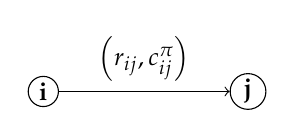
\begin{tikzpicture}[nodes={font=\bf\small}, scale=0.65]
%  \draw [help lines] (-1,-1) grid (8,5);o

\tikzstyle{tasknode}=[%
  draw,
  circle,
  minimum width=0.4,
  inner sep=0.5mm,
]

% nodes
\node [tasknode] (i) at (0, 0) {i};
\node [tasknode] (j) at (4, 0) {j};

\path [draw, ->] (i) -- node[above] {$\left(r_{ij},c_{ij}^{\pi}\right)$} (j);

\end{tikzpicture} 
%%%%%%%%%%%%%%%%%%%%%%%%%%%%%%%%%%%%%%%%%%%

        \caption{Notation: each arc is labelled with residual capacity and reduced cost.} 
    \end{subfigure}
    \begin{subfigure}[c]{0.5\textwidth}
        %%%%%%%%%%%%%%%%%%%%%%%%%%%%%%%%%%%%%%%%%%%
\begin{tikzpicture}[nodes={font=\bf\small}, scale=0.45]
%  \draw [help lines] (-1,-1) grid (8,5);o

\tikzstyle{mynode}=[%
  draw,
  circle,
  minimum width=0.4,
  inner sep=0.5mm,
]

\tikzstyle{myarc}=[%
  draw,
  arrows={-Triangle[scale=1]},
  line width=1pt,
]

% nodes
\node [mynode] (a) at (0, 4) {A};
\node [mynode] (b) at (4, 8) {B};
\node [mynode] (c) at (4, 0) {C};
\node [mynode] (d) at (8, 4) {D};

% excesses
\node [left=0.5cm] at (0,4.3) {$e_A = 3$}; % A
\node [above=0.6cm] at (4,8) {$e_B = 0$}; % B
\node [below=0.2cm] at (4,0) {$e_C = 0$}; % C
\node [right=0.5cm] at (8,4.3) {$e_D = -3$}; % D

% potentials
\node [left=0.5cm] at (0,3.7) {$\pi_A = 0$}; % A
\node [above=0.15cm] at (4,8) {$\pi_B = 0$}; % B
\node [below=0.65cm] at (4,0) {$\pi_C = 0$}; % C
\node [right=0.5cm] at (8,3.7) {$\pi_D = 0$}; % D

\path [myarc] (a) -- node[above, sloped] {$(2,1)$} (b);
\path [myarc] (a) -- node[below, sloped] {$(3,5)$} (c);
\path [myarc] (b) -- node[right] {$(5,10)$} (c);
\path [myarc] (b) -- node[above, sloped] {$(1,1)$} (d);
\path [myarc] (c) -- node[below, sloped] {$(5,1)$} (d);

\end{tikzpicture} 

        \caption{Initial network.}
    \end{subfigure}
    \begin{subfigure}[c]{0.5\textwidth}
        %%%%%%%%%%%%%%%%%%%%%%%%%%%%%%%%%%%%%%%%%%%
\begin{tikzpicture}[nodes={font=\bf\small}, scale=0.45]
%  \draw [help lines] (-1,-1) grid (8,5);o

\tikzstyle{mynode}=[%
  draw,
  circle,
  minimum width=0.4,
  inner sep=0.5mm,
]

\tikzstyle{myarc}=[%
  draw,
  arrows={-Triangle[scale=1]},
  line width=1pt,
]

% nodes
\node [mynode] (a) at (0, 4) {A};
\node [mynode] (b) at (4, 8) {B};
\node [mynode] (c) at (4, 0) {C};
\node [mynode] (d) at (8, 4) {D};

% excesses
\node [left=0.5cm] at (0,4.3) {$e_A = 3$}; % A
\node [above=0.6cm] at (4,8) {$e_B = 0$}; % B
\node [below=0.2cm] at (4,0) {$e_C = 0$}; % C
\node [right=0.5cm] at (8,4.3) {$e_D = -3$}; % D

% s=A, t=D
% shortest paths:
% B: A->B (1)
% C: A->C (5)
% D : A->B->D (2)

% potentials
\node [left=0.5cm] at (0,3.7) {$\pi_A = 0$}; % A
\node [above=0.15cm] at (4,8) {$\pi_B = -1$}; % B
\node [below=0.65cm] at (4,0) {$\pi_C = -5$}; % C
\node [right=0.5cm] at (8,3.7) {$\pi_D = -2$}; % D

% (cap,cost)
\path [myarc] (a) -- node[above, sloped] {$(2,0)$} (b);
\path [myarc] (a) -- node[below, sloped] {$(3,0)$} (c);
\path [myarc] (b) -- node[right] {$(5, 6)$} (c);
\path [myarc] (b) -- node[above, sloped] {$(1,0)$} (d);
\path [myarc] (c) -- node[below, sloped] {$(5,4)$} (d);

\end{tikzpicture} 

        \caption{SSSP problem solved from \textbf{A}, and potentials updated.}
        \label{fig:ssp-trace:first-pi}
    \end{subfigure}
    \begin{subfigure}[c]{0.5\textwidth}
        %%%%%%%%%%%%%%%%%%%%%%%%%%%%%%%%%%%%%%%%%%%
\begin{tikzpicture}[nodes={font=\bf\small}, scale=0.45]
%  \draw [help lines] (-1,-1) grid (8,5);o

\tikzstyle{mynode}=[%
  draw,
  circle,
  minimum width=0.4,
  inner sep=0.5mm,
]

\tikzstyle{myarc}=[%
  draw,
  arrows={-Triangle[scale=1]},
  line width=1pt,
]

% nodes
\node [mynode] (a) at (0, 4) {A};
\node [mynode] (b) at (4, 8) {B};
\node [mynode] (c) at (4, 0) {C};
\node [mynode] (d) at (8, 4) {D};

% excesses
\node [left=0.3cm] at (0,4.5) {$e_A = 2$}; % A
\node [above=0.6cm] at (4,8) {$e_B = 0$}; % B
\node [below=0.2cm] at (4,0) {$e_C = 0$}; % C
\node [right=0.3cm] at (8,4.5) {$e_D = -2$}; % D

% s=A, t=D
% shortest paths:
% B: A->B (1)
% C: A->C (5)
% D : A->B->D (2)

% potentials
\node [left=0.3cm] at (0,3.5) {$\pi_A = 0$}; % A
\node [above=0.15cm] at (4,8) {$\pi_B = -1$}; % B
\node [below=0.65cm] at (4,0) {$\pi_C = -5$}; % C
\node [right=0.3cm] at (8,3.5) {$\pi_D = -2$}; % D

% (cap,cost)
\path [myarc] (a) -- node[above, sloped] {$(1,0)$} (b);
\path [myarc] (b) edge[bend left=20, looseness=1] node[below, sloped] {$(1,0)$} (a);
\path [myarc] (a) -- node[below, sloped] {$(3,0)$} (c);
\path [myarc] (b) -- node[right] {$(5, 6)$} (c);
\path [myarc] (d) -- node[above, sloped] {$(1,0)$} (b);
\path [myarc] (c) -- node[below, sloped] {$(5,4)$} (d);

\end{tikzpicture} 
%%%%%%%%%%%%%%%%%%%%%%%%%%%%%%%%%%%%%%%%%%%

        \label{fig:ssp-trace:first-augment}                
        \caption{Flow augmented along shortest path $A \to B \to D$.}
    \end{subfigure}
    \begin{subfigure}[c]{0.5\textwidth}
        %%%%%%%%%%%%%%%%%%%%%%%%%%%%%%%%%%%%%%%%%%%
\begin{tikzpicture}[nodes={font=\bf\small}, scale=0.45]
%  \draw [help lines] (-1,-1) grid (8,5);o

\tikzstyle{mynode}=[%
  draw,
  circle,
  minimum width=0.4,
  inner sep=0.5mm,
]

\tikzstyle{myarc}=[%
  draw,
  arrows={-Triangle[scale=1]},
  line width=1pt,
]

% nodes
\node [mynode] (a) at (0, 4) {A};
\node [mynode] (b) at (4, 8) {B};
\node [mynode] (c) at (4, 0) {C};
\node [mynode] (d) at (8, 4) {D};

% excesses
\node [left=0.5cm] at (0,4.5) {$e_A = 0$}; % A
\node [above=0.6cm] at (4,8) {$e_B = 0$}; % B
\node [below=0.2cm] at (4,0) {$e_C = 0$}; % C
\node [right=0.5cm] at (8,4.5) {$e_D = 0$}; % D

% s=A, t=D
% shortest paths:
% B: A->B (0)
% C: A->C (0)
% D: A->C->B (4)

% potentials
\node [left=0.5cm] at (0,3.5) {$\pi_A = 0$}; % A
\node [above=0.15cm] at (4,8) {$\pi_B = -1$}; % B
\node [below=0.65cm] at (4,0) {$\pi_C = -5$}; % C
\node [right=0.5cm] at (8,3.5) {$\pi_D = -6$}; % D

% (cap,cost)
\path [myarc] (a) -- node[above, sloped] {$(1,0)$} (b);
\path [myarc] (b) edge[bend left=20, looseness=1] node[below, sloped] {$(1,0)$} (a);
\path [myarc] (a) -- node[below, sloped] {$(3,0)$} (c);
\path [myarc] (b) -- node[right] {$(5, 6)$} (c);
\path [myarc] (d) -- node[above, sloped] {$(1,4)$} (b);
\path [myarc] (c) -- node[below, sloped] {$(5,0)$} (d);

\end{tikzpicture} 
%%%%%%%%%%%%%%%%%%%%%%%%%%%%%%%%%%%%%%%%%%%

        \caption{SSSP problem solved from \textbf{A}, and potentials updated.}
        \label{fig:ssp-trace:second-pi}
    \end{subfigure}
    \begin{subfigure}[c]{0.5\textwidth}
        %%%%%%%%%%%%%%%%%%%%%%%%%%%%%%%%%%%%%%%%%%%
\begin{tikzpicture}[nodes={font=\bf\small}, scale=0.45]
%  \draw [help lines] (-1,-1) grid (8,5);o

\tikzstyle{mynode}=[%
  draw,
  circle,
  minimum width=0.4,
  inner sep=0.5mm,
]

\tikzstyle{myarc}=[%
  draw,
  arrows={-Triangle[scale=1]},
  line width=1pt,
]

% nodes
\node [mynode] (a) at (0, 4) {A};
\node [mynode] (b) at (4, 8) {B};
\node [mynode] (c) at (4, 0) {C};
\node [mynode] (d) at (8, 4) {D};

% excesses
\node [left=0.5cm] at (0,4.3) {$e_A = 2$}; % A
\node [above=0.6cm] at (4,8) {$e_B = 0$}; % B
\node [below=0.2cm] at (4,0) {$e_C = 0$}; % C
\node [right=0.5cm] at (8,4.3) {$e_D = -2$}; % D

% s=A, t=D
% shortest paths:
% B: A->B (0)
% C: A->C (0)
% D: A->C->B (4)

% potentials
\node [left=0.5cm] at (0,3.7) {$\pi_A = 0$}; % A
\node [above=0.15cm] at (4,8) {$\pi_B = -1$}; % B
\node [below=0.65cm] at (4,0) {$\pi_C = -5$}; % C
\node [right=0.5cm] at (8,3.7) {$\pi_D = -6$}; % D

% (cap,cost)
\path [myarc] (a) -- node[above, sloped] {$(1,0)$} (b);
\path [myarc] (b) edge[bend left=20, looseness=1] node[below, sloped] {$(1,0)$} (a);
\path [myarc] (a) -- node[below, sloped] {$(1,0)$} (c);
\path [myarc] (c) edge[bend right=20, looseness=1] node[above, sloped] {$(2,0)$} (a);
\path [myarc] (b) -- node[above right] {$(5, 6)$} (c);
\path [myarc] (d) -- node[above, sloped] {$(1,4)$} (b);
\path [myarc] (c) -- node[below, sloped] {$(3,0)$} (d);
\path [myarc] (d) edge[bend right=20, looseness=1] node[above, sloped] {$(2,0)$} (c);

\end{tikzpicture} 
%%%%%%%%%%%%%%%%%%%%%%%%%%%%%%%%%%%%%%%%%%%

        \label{fig:ssp-trace:second-augment}        
        \caption{Flow augmented along shortest path $A \to C \to D$.}
    \end{subfigure}
    \caption[Successive shortest path algorithm in action]{Step-by-step trace of the successive shortest path algorithm in action, depicting the residual network. Each node $i$ is labelled with its excess $e_i$ and potential $\pi_i$.}
    \label{fig:ssp-trace}
\end{figure}

% SOMEDAY: footnote after $t$ is bad
\begin{algorithm}
    \caption{Successive shortest path}
    \label{algo:successive-shortest-path}
    \begin{algorithmic}[1]
        \State $\mathbf{x} \gets \mathbf{0}$ and $\boldsymbol{\pi} \gets \mathbf{0}$
        \While{mass balance constraints not satisfied} \label{algo:successive-shortest-path:start-loop}
          \State choose excess vertex $s$ and deficit vertex $t$\footnotemark \label{algo:successive-shortest-path:select-active}
          % SOMEDAY: These statements are multi-line, shorten? Or at least reflow.
          \State solve SSSP problem from $s$ to all vertices in the residual network $G_{\mathbf{x}}$, with respect to the reduced costs $c^{\boldsymbol{\pi}}_{ij}$ \label{algo:successive-shortest-path:solve-sssp}
          \State let $\mathbf{d}$ denote the vector of shortest path distances, such that $d_i$ is the shortest path from $s$ to $i\in V$
          \Let{$\boldsymbol{\pi}$}{$\boldsymbol{\pi} - \mathbf{d}$} \label{algo:successive-shortest-path:update-potentials}
          \State let $P$ denote a shortest path from $s$ to $t$
          \Let{$\delta$}{$\min\left(e_s, -e_t, \min\left\{ r_{ij} \::\: (i,j) \in P\right\}\right)$} \label{algo:successive-shortest-path:compute-delta}
          \State augment $\delta$ units of flow along path $P$ \label{algo:successive-shortest-path:augment-flow}
        \EndWhile \label{algo:successive-shortest-path:end-loop}
    \end{algorithmic}
\end{algorithm}

\footnotetext{Note so long as the mass balance constraints are unsatisfied, there must exist both an excess vertex $s$ and deficit vertex $t$. This is because the total sum of excesses must equal the total sum of deficits for any feasible problem.}

The successive shortest path algorithm maintains a pseudoflow $\mathbf{x}$ (see \cref{sec:prep-flow-pseudo}) and potentials $\boldsymbol{\pi}$ satisfying reduced cost optimality (see \cref{thm:optimality-reduced-cost}), and attempts to attain feasibility. This is in contrast to the cycle cancelling algorithm, which maintains feasibility and strives to achieve optimality.

Each iteration of the algorithm identifies an excess vertex $s$ and excess vertex $t$. Next, the single-source shortest-path (SSSP) problem~\cite[ch.~24]{CLRS:2009} is solved from $s$. To maintain reduced cost optimality, the potentials $\boldsymbol{\pi}$ are updated. Finally, the pseudoflow $\mathbf{x}$ is augmented along a shortest path $P$ from $s$ to $t$. The algorithm terminates when no excess or deficit vertices exist.

The amount of flow $\delta$ sent over the path is limited by the minimum residual capacity of arcs along $P$. $\delta$ is further restricted so that a non-negative supply at $s$ and demand at $t$ are maintained. This guarantees the excess at supply vertices and deficit at demand vertices is monotonically decreasing, ensuring each iteration improves the feasibility of the flow.

\Cref{fig:ssp-trace} illustrates the operation of successive shortest path. Note that updating the potentials in \cref{fig:ssp-trace:first-pi,fig:ssp-trace:second-pi} makes the reduced cost of arcs in the shortest-path tree rooted at \textbf{A} zero, allowing the flow to be augmented in \cref{fig:ssp-trace:first-augment,fig:ssp-trace:second-augment} without violating reduced cost optimality.

\subsection{Optimisations} \label{sec:impl-ssp-optimisations}

\subsubsection{Choice of shortest-path algorithm}
The fastest known single-source shortest-path algorithms are all variants of Djikstra's algorithm~\cite[ch.~4]{Ahuja:1993}, differing in the underlying heap data structure used. The asymptotically fastest are based on Fibonacci heaps, with a complexity of $O(m + n\lg n)$. By contrast, Djikstra's algorithm has a complexity of $O(m\lg n)$ when using the popular binary heap data structure\footnotemark.
\footnotetext{Although binary and Fibonacci heaps have the same asymptotic complexity on flow scheduling networks, since $m = O(n)$ by \cref{lemma:network-num-arcs}.} 

However, computational benchmarks have found Fibonacci heaps to be slower than binary heaps in practice, except on extremely large graphs~\cite[p.~15]{KiralyKovacs:2012}. In light of this, I used a binary heap implementation in this project.

\subsubsection{Terminating Djikstra's algorithm early}

Djikstra's algorithm is said to have \emph{permanently labelled} a vertex $i$ when it extracts $i$ from the heap. At this point, Djikstra has found a shortest path from $s$ to $i$. I modified the successive shortest path algorithm to terminate Djikstra as soon as it permanently labels a deficit vertex $l$: details of the implementation and a proof of correctness are given in \cref{appendix:impl-ssp:partial-djikstra}.

\subsection{Analysis} \label{sec:impl-ssp-analysis}

\begin{restatable}[Loop invariant of successive shortest path]{thm}{sspinvariant} \label{thm:ssp-invariant}
    Immediately before each iteration of the loop, $(\mathbf{x},\boldsymbol{\pi})$ satisfies reduced cost optimality.
\end{restatable}
\begin{proof}
See \cref{appendix:impl-ssp:analysis-correctness}.
\end{proof}
\begin{restatable}[Correctness of successive shortest path]{cor}{sspcorrectness} \label{cor:ssp-correctness}
    Upon termination, $\mathbf{x}$ is a solution to the minimum-cost flow problem.
\end{restatable}
\begin{proof}
See \cref{appendix:impl-ssp:analysis-correctness}.
\end{proof}

\begin{thm}[Asymptotic complexity of generic successive shortest path] \label{thm:ssp-complexity}
Let $S(n,m,C)$ denote the time complexity of solving a single-source shortest path problem (SSSP) with non-negative arc costs, bounded above by $C$, over a network with $n$ vertices and $m$ arcs. Then the time complexity of successive shortest path is $O(nUS(n,m,C))$.
\end{thm}
\begin{proof}
Each iteration of the loop body (\crefrange{algo:successive-shortest-path:start-loop}{algo:successive-shortest-path:end-loop} of \cref{algo:successive-shortest-path}) decreases the excess of vertex $s$ by $\delta$ and the deficit of vertex $t$ by $\delta$, while leaving the excess/deficit of other vertices unchanged. Prior to the iteration, $e_s \geq 0$ and $e_t \leq 0$, so the total excess and total deficit in the network are both decreased by $\delta$. By \cref{assumption:integrality}, $\delta \geq 1$. Thus the number of iterations is bounded by the initial total excess. This in turn is bounded by $nU/2 = O(nU)$. So there are $O(nU)$ iterations in total.

Within each iteration, the algorithm solves an SSSP problem on \cref{algo:successive-shortest-path:solve-sssp}. Since reduced cost optimality is maintained throughout the algorithm, the arc costs in the shortest-path problem are non-negative\footnotemark. Thus the cost of solving this problem is $S(n,m,C)$.
\footnotetext{Algorithms such as Djikstra which assume non-negative arc lengths are asymptotically faster than more general algorithms such as Bellman-Ford.}

The cost of \cref{algo:successive-shortest-path:select-active,algo:successive-shortest-path:update-potentials} are clearly $O(n)$. \Cref{algo:successive-shortest-path:compute-delta,algo:successive-shortest-path:augment-flow} are also $O(n)$, since the length of $P$ is bounded by $n-1$ (shortest paths are acyclic). Certainly $S(n,m,C) = \Omega(n)$, so the cost of each iteration is $O(S(n,m,C))$.

It follows that the overall time complexity of the algorithm is $O(nUS(n,m,C))$.
\end{proof}

\begin{cor}[Asymptotic complexity of successive shortest path in Hapi]
The implementation in this project has a time complexity of $O(nmU \lg n)$.
\end{cor}
\begin{proof}
Djikstra's algorithm with a binary heap data structure is used to solve the SSSP problem, giving $S(n,m,C) = O(m \lg n)$. The result follows by \cref{thm:ssp-complexity}.
\end{proof}

\begin{remark} \label{remark:ssp-flow-scheduling-complexity}
On flow scheduling networks, no vertex has a greater than unit supply by \cref{lemma:network-supply}. This gives a bound on the total excess of $O(n)$ rather than $O(nU)$. Moreover, by \cref{lemma:network-num-arcs}, $m = O(n)$. So the complexity improves to $O(n^2 \lg n)$.
\end{remark}

\section{Relaxation algorithm} \label{sec:impl-relax}

% PROOFREAD: 1 minor edits

Like the successive shortest path algorithm, the relaxation algorithm works by augmenting along shortest paths in the residual network from excess vertices to deficit vertices. Unlike successive shortest path, it uses intermediate information to update vertex potentials as it constructs the shortest-path tree. It is inspired by Lagrangian relaxation~\cite[ch.~16]{Ahuja:1993}\cite{Fisher:1981}.

Relaxation performs much better empirically than the successive shortest path algorithm, and is one of the fastest algorithms for some classes of flow networks~\cite{KiralyKovacs:2012}. However, its worst-case complexity is exponential, slower than any other algorithm considered in this dissertation\footnotemark. Like successive shortest path, it is well suited to incremental operation, but is inappropriate for an approximate solver.
\footnotetext{The generic version of cycle cancelling is also exponential in the worst-case, however there are variants with a strongly polynomial bound. By contrast, there are no variants of relaxation achieving polynomial time, although in practice exponential runtime is not observed on realistic flow networks.}

% WORDCOUNT: Relaxation -- could move introductory proofs to appendix
% They are mostly your own, but not especially enlightening or difficult.
% Definitely keep the statements here, though, they're pretty important.
\subsection{The relaxed integer programming problem}
Before describing how the relaxation algorithm works, it is necessary to understand the problem it seeks to optimise. I have previously discussed the primal (see \cref{sec:prep-flow-mcf}) and dual (see \cref{sec:prep-flow-rc-and-dual}) versions of the minimum-cost flow problem. The relaxed version of the problem can be derived by applying Lagrangian relaxation to the primal problem, and has characteristics of both the primal and dual formulations. It is denoted by $\mathrm{LR}(\boldsymbol{\pi})$, and is defined by:

\begin{equation} \label{eq:relax-obj-fun-excess}
\mathrm{maximise}\: w\left(\boldsymbol{\pi}\right)=\min_{x}\left[\sum_{\left(i,j\right)\in E}c_{ij}x_{ij}+\sum_{i\in V}\boldsymbol{\pi}_{i}e_{i}\right]
\end{equation}
where $\mathbf{x}$ is subject to the capacity constraints first given in \cref{eq:capacity-constraints}:
\[\forall\left(i,j\right)\in E\cdot 0\leq x_{ij}\leq u_{ij}.\]

\begin{lemma}
An equivalent definition for $w(\boldsymbol{\pi})$ is:
\begin{equation} \label{eq:relax-obj-fun-balance}
w(\boldsymbol{\pi})=\min_{x}\left[\sum_{\left(i,j\right)\in E}c_{ij}^{\boldsymbol{\pi}}x_{ij}+\sum_{i\in V}\pi_{i}b_{i}\right].
\end{equation}
\end{lemma}
\begin{proof}
Recall the excess at vertex $i$ is defined as:
\[e_{i}=b_{i}+\sum_{(j,i)\in E}x_{ji}-\sum_{(i,j)\in E}x_{ij}\]
So:
\begin{align*}
w\left(\pi\right)= & \min_{x}\left[\sum_{\left(i,j\right)\in E}c_{ij}x_{ij}+\sum_{i\in V}\pi_{i}\left(b_{i}+\sum_{(j,i)\in E}x_{ji}-\sum_{(i,j)\in E}x_{ij}\right)\right]\:\mbox{substituting for }e_{i};\\
= & \min_{x}\left[\sum_{\left(i,j\right)\in E}c_{ij}x_{ij}+\sum_{i\in V}\pi_{i}b_{i}+\sum_{i\in V}\pi_{i}\sum_{(j,i)\in E}x_{ji}-\sum_{i\in V}\pi_{i}\sum_{(i,j)\in E}x_{ij}\right]\:\mbox{expanding;}\\
= & \min_{x}\left[\sum_{\left(i,j\right)\in E}c_{ij}x_{ij}+\sum_{i\in V}\pi_{i}b_{i}+\sum_{(j,i)\in E}\pi_{i}x_{ji}-\sum_{(i,j)\in E}\pi_{i}x_{ij}\right]\:\mbox{double to single sum;}\\
= & \min_{x}\left[\sum_{\left(i,j\right)\in E}c_{ij}x_{ij}+\sum_{i\in V}\pi_{i}b_{i}+\sum_{(i,j)\in E}\pi_{j}x_{ij}-\sum_{(i,j)\in E}\pi_{i}x_{ij}\right]\:\mbox{permuting \ensuremath{i} and \ensuremath{j} in 3rd sum;}\\
= & \min_{x}\left[\sum_{\left(i,j\right)\in E}\left(c_{ij}-\pi_{i}+\pi_{j}\right)x_{ij}+\sum_{i\in V}\pi_{i}b_{i}\right]\:\mbox{factoring;}\\
= & \min_{x}\left[\sum_{\left(i,j\right)\in E}c_{ij}^{\boldsymbol{\pi}}x_{ij}+\sum_{i\in V}\pi_{i}b_{i}\right]\:\mbox{substituting reduced cost.}
\end{align*}
\end{proof}

\begin{remark}
Note that \cref{eq:relax-obj-fun-excess} is expressed in terms of the excesses ($\mathbf{x}$-dependent) and arc costs, whereas \cref{eq:relax-obj-fun-balance} is expressed in terms of the reduced costs ($\boldsymbol{\pi}$-dependent) and balances.\\
\end{remark}

\begin{lemma} \label{lemma:relax-rc-lr-equivalence}
Let $\mathbf{x}$ be a pseudoflow and $\boldsymbol{\pi}$ vertex potentials. Then $\left(\mathbf{x},\boldsymbol{\pi}\right)$ satisfies reduced cost optimality conditions if and only if $\mathbf{x}$ is an optimal solution to $\mathrm{LR}(\boldsymbol{\pi})$.
\end{lemma}
\begin{proof}
The complementary slackness conditions will be used rather than reduced cost optimality conditions, to simplify the proof. Recall the two conditions are equivalent (see \cref{sec:prep-flow-optimality}).

By the definition of the relaxed problem and  \cref{eq:relax-obj-fun-balance}, $\mathbf{x}$ is an optimal solution to $\mathrm{LR}(\boldsymbol{\pi})$ if and only if it minimises:
\[\sum_{\left(i,j\right)\in E}c_{ij}^{\boldsymbol{\pi}}x_{ij}+\sum_{i\in V}\pi_{i}b_{i}\]
subject to the capacity constraints of \cref{eq:capacity-constraints}.

The second sum, $\sum_{i \in V} \pi_i b_i$, is constant in $\mathbf{x}$. Thus $\mathbf{x}$ is an optimal solution to $\mathrm{LR}(\boldsymbol{\pi})$ if and only if it minimises:
\[\sum_{\left(i,j\right)\in E}c_{ij}^{\boldsymbol{\pi}}x_{ij}\]

Note the coefficients $c_{ij}^{\boldsymbol{\pi}}$ are constant in $\mathbf{x}$. Furthermore, each term is independent of the others: by varying $x_{ij}$, only the term $c_{ij}^{\boldsymbol{\pi}}x_{ij}$ is affected\footnotemark. Thus the sum is minimised when each of its summands is minimised.
\footnotetext{Contrast this to if we were varying a vertex quantity, such as $\pi_i$, which would affect many arcs.}

When $c_{ij}^{\boldsymbol{\pi}}>0$, the term $c_{ij}^{\boldsymbol{\pi}}x_{ij}$ is minimised by setting $x_{ij}$ to the smallest value permitted by \cref{eq:capacity-constraints}, which is zero. When $c_{ij}^{\boldsymbol{\pi}}<0$, set $x_{ij}$ to the largest possible value, $u_{ij}$. When $c_{ij}^{\boldsymbol{\pi}}=0$, the choice of $x_{ij}$ is arbitrary. This is the same as the complementary slackness conditions given in \cref{thm:optimality-complementary-slackness}. 

Thus complementary slackness optimality is equivalent to $\mathbf{x}$ being an optimal solution to $\mathrm{LR}(\boldsymbol{\pi})$. The result follows by equivalence of reduced cost optimality and complementary slackness optimality.
\end{proof}

\begin{defn}
Let $z^*$ denote the optimal objective function value of the minimum-cost flow problem, that is the cost of an optimal flow. \\
\end{defn}

\begin{lemma} \label{lemma:relax-dual-optimality}
~ % force line break
\begin{enumerate}[label=(\alph*)]
    \item For any potential vector $\boldsymbol{\pi}$, $w(\boldsymbol{\pi}) \leq z^*$.
    \item There exists vertex potentials $\boldsymbol{\pi}^*$ for which $w(\boldsymbol{\pi}^*) = z^*$.
\end{enumerate}
\end{lemma}
\begin{proof} (Adapted from Ahuja \textit{et al.}~\cite[lemma.~9.16]{Ahuja:1993})
    
For the first part, let $\mathbf{x}^*$ be a feasible flow with objective function value $s(\mathbf{x}^*) = z^*$: that is, $\mathbf{x}^*$ is a solution to the minimum-cost flow problem given in \cref{eq:mcf-primal-problem}.

Using the form of $w(\boldsymbol{\pi})$ stated in \cref{eq:relax-obj-fun-excess}, it follows that:
\[w(\boldsymbol{\pi})\leq\sum_{\left(i,j\right)\in E}c_{ij}x_{ij}^{*}+\sum_{i\in V}\pi_{i}e_{i}\]
by dropping the $\min_x$ and replacing $=$ with $\leq$.

Note that the first sum is equal to $s(\mathbf{x}^*) = z^*$. Since $\mathbf{x}^*$ is a feasible flow, the mass balance constraints are satisfied, so:
\[\forall i \in V\cdot e_i = 0\]
and thus the second sum is equal to $0$. It follows that:
\[w(\boldsymbol{\pi}) \leq z^* + 0 = z^*\]

To prove the second part, let $\boldsymbol{\pi}^*$ be vertex potentials such that $\left(\mathbf{x}^*,\boldsymbol{\pi}^*\right)$ satisfy the reduced cost optimality conditions given in \cref{eq:optimality-reduced-cost}\footnotemark. By \cref{lemma:relax-rc-lr-equivalence}, it follows that $\mathbf{x}^*$ is an optimal solution to $\mathrm{LR}(\boldsymbol{\pi}^*)$. Thus $w(\boldsymbol{\pi}^*) = z^*$.
\footnotetext{Note such a choice of $\boldsymbol{\pi}^*$ is guaranteed to exist since $\mathbf{x}^*$ is an optimal solution to the minimum-cost flow problem.}
\end{proof}

% Highlight similarity to weak dulity theorem?

\subsection{Algorithm description}

The algorithm maintains a pseudoflow $\mathbf{x}$ and vertex potentials $\boldsymbol{\pi}$, such that $\mathbf{x}$ is an optimal solution to $\mathrm{LR}(\boldsymbol{\pi})$. Equivalently, by \cref{lemma:relax-rc-lr-equivalence}, $\left(\mathbf{x},\boldsymbol{\pi}\right)$ satisfies reduced cost optimality.

While the pseudoflow $\mathbf{x}$ is infeasible, the algorithm selects an excess vertex $s$. It then builds a tree in the residual network $G_{\mathbf{x}}$, rooted at $s$. Only arcs with zero reduced cost are added to the tree, hence it is a shortest-path tree.

The algorithm can perform one of two operations, described below. An operation is run as soon as its precondition is satisfied. After it executes, the tree is destroyed and the process repeats.

The first operation is to \emph{update the potentials}, increasing the value of the objective function while maintaining optimality. That, is $\boldsymbol{\pi}$ is updated to $\boldsymbol{\pi}'$ such that $w\left(\boldsymbol{\pi}'\right) > w\left(\boldsymbol{\pi}\right)$ and $\mathbf{x}$ is updated to $\mathbf{x}'$ such that $\mathbf{x}'$ is an optimal solution to $\mathrm{LR}(\boldsymbol{\pi}')$.

The second operation is to \emph{augment the flow} $\mathbf{x}$, while leaving potentials $\boldsymbol{\pi}$ unchanged. The new flow $\mathbf{x}'$ remains an optimal solution of $\mathrm{LR}(\boldsymbol{\pi})$, and improves feasibility.

The primary goal of the algorithm is thus to increase the value of the objective function, while the secondary goal is to increase feasibility (leaving the objective function unchanged). Therefore, when both operations are eligible to be executed, updating the potentials is preferred. 

A few definitions are necessary before specifying the preconditions for these operations.\\

\begin{defn}[Tree excess] \label{defn:relax-tree-excess}
Let $S$ denote the set of vertices spanned by the tree. Define:
\begin{equation} \label{eq:relax-tree-excess}
e(S) = \sum_{i \in S} e_i
\end{equation}
\end{defn}

\begin{defn}[Cuts] \label{defn:relax-cuts}
A \emph{cut} of a graph $G = (V,E)$ is a partition of $V$ into two sets: $S$ and $\overline{S} = V \setminus S$. We denote the cut by $\left[S,\overline{S}\right]$. Let $\left(S,\overline{S}\right)$ and $\left(\overline{S},S\right)$ denote the set of forward and backward arcs crossing the cut, respectively. Formally:
\[\left(S,\overline{S}\right) = \set{(i,j) \in E | i \in S \land j \in \overline{S}}\]
\[\left(\overline{S},S\right) = \set{(i,j) \in E | i \in \overline{S} \land j \in S}\]
\end{defn}

\begin{defn} \label{defn:relax-tree-residual}
Let:
\begin{equation} \label{eq:relax-tree-residual}
r(\boldsymbol{\pi},S) = \sum_{(i,j) \in \left(S,\overline{S}\right) \land c_{ij}^{\boldsymbol{\pi}}} r_{ij}
\end{equation}
\end{defn}

\begin{remark}
Since the tree only ever contains arcs of zero reduced cost, $r(\boldsymbol{\pi},S)$ represents the total residual capacity of the arcs which are eligible for addition to the tree in the current iteration.
\end{remark}

\begin{algorithm}
    \caption{Relaxation: main procedure}
    \label{algo:relaxation}
    \begin{algorithmic}[1]
        \State $\mathbf{x} \gets \mathbf{0}$ and $\boldsymbol{\pi} \gets \mathbf{0}$ \label{algo:relaxation:initialisation}
        \While{network contains an excess vertex $s$} \label{algo:relaxation:outer-loop-start}
        \Let{$S$}{$\Set{s}$}
        \State initialise $e(S)$ and $r(\boldsymbol{\pi},S)$
        \If{$e(S) > r(\boldsymbol{\pi},S)$}
        \Call{UpdatePotentials}{} \label{algo:relaxation:first-update-potentials}
        \EndIf
        \While{$e(S) \leq r(\boldsymbol{\pi},S)$}
        \label{algo:relaxation:inner-loop-start}
        \State select arc $(i,j) \in \left(S,\overline{S}\right)$ in the residual network with $c_{ij}^{\boldsymbol{\pi}}=0$ \label{algo:relaxation:select-arc}
        \If{$e_j \geq 0$} \label{algo:relaxation:if-source}
        \Let{$\mathrm{Pred}_j$}{$i$} \label{algo:relaxation:update-predecessor}
        \Let{$S$}{$S \cup \Set{j}$} \label{algo:relaxation:add-vertex}
        \State update $e(S)$ and $r(\boldsymbol{\pi},S)$ 
        \label{algo:relaxation:end-if-source}
        \Else
        \State \Call{AugmentFlow}{j} \label{algo:relaxation:augment}
        \Break
        \EndIf
        \EndWhile \label{algo:relaxation:inner-loop-end}
        \If{$e(S) > r(\boldsymbol{\pi},S)$}
        \Call{UpdatePotentials}{} \label{algo:relaxation:second-update-potentials}
        \EndIf
        \EndWhile \label{algo:relaxation:outer-loop-end}
    \end{algorithmic}
\end{algorithm}

\begin{algorithm}
    \caption{Relaxation: potential update procedure}
    \label{algo:relaxation-update-potentials}
    \begin{algorithmic}[1]
        \Require $e(S) > r(\boldsymbol{\pi},S)$
        \Statex
        \Function{UpdatePotentials}{}
        \For{every arc $(i,j) \in \left(S,\overline{S}\right)$ in the residual network with $c_{ij}^{\boldsymbol{\pi}}=0$} \label{algo:relaxation-update-potentials:saturate-loop}
        \State saturate arc $(i,j)$ by sending $r_{ij}$ units of flow \label{algo:relaxation-update-potentials:saturate-cmd}
        \EndFor
        \State compute $\alpha \gets \min\set{c_{ij}^{\boldsymbol{\pi}} | (i,j)\in\left(S,\overline{S}\right)\mbox{ and }r_{ij}>0}$
        \label{algo:relaxation-update-potentials:compute-alpha}
        \For{every vertex $i\in S$}
        \label{algo:relaxation-update-potentials:update-loop}
        \Let{$\pi_i$}{$\pi_i + \alpha$}
        \label{algo:relaxation-update-potentials:update-cmd}
        \EndFor
        \EndFunction
    \end{algorithmic}
\end{algorithm}

\begin{algorithm}
    \caption{Relaxation: flow augmentation procedure}
    \label{algo:relaxation-augment-flow}
    \begin{algorithmic}[1]
        \Require $e(S) \leq r(\boldsymbol{\pi},S)$ and $e_t < 0$
        \Statex
        \Function{AugmentFlow}{t}
        \State chase predecessors in $\mathrm{Pred}$ starting from $t$ to find a shortest path $P$ from $s$ to $t$ \label{algo:relaxation-augment-flow:find-P}
        \Let{$\delta$}{$\min\left(e_s, -e_t, \min\Set{ r_{ij} | (i,j) \in P}\right)$} \label{algo:relaxation-augment-flow:compute-delta}
        \State augment $\delta$ units of flow along path $P$ \label{algo:relaxation-augment-flow:augment-path}
        \EndFunction
    \end{algorithmic}
\end{algorithm}

\Cref{algo:relaxation,algo:relaxation-update-potentials,algo:relaxation-augment-flow} formally describe the solution method. A set $S$ of vertices spanned by the shortest path tree is maintained. The arcs in the tree are specified by the predecessor array, $\mathrm{Pred}$. Although $e(S)$ and $r(\boldsymbol{\pi},S)$ could be computed when needed, they are more efficiently maintained as variables, being updated whenever a vertex is added to the tree.

Each iteration of the outer loop of \cref{algo:relaxation} selects an excess vertex, $s$, to be the root of a new tree. The inner loop adds vertices and arcs to this tree. If a deficit vertex $t$ is encountered, flow is augmented along the (zero-cost) shortest path discovered from $s$ to $t$, and the inner loop terminates. However, an iteration may end before this: if at any point $e(S) > r(\boldsymbol{\pi},S)$, the potentials are updated, and a new iteration starts\footnotemark.
\footnotetext{Note \cref{algo:relaxation:first-update-potentials} of \cref{algo:relaxation} is just an optimisation.}

\subsection{Analysis} \label{sec:impl-relax-analysis}

%\begin{restatable}[Correctness of cycle cancelling]{thm}{correctnesscc}
%    \label{thm:cycle-cancelling-correctness}
%    Upon termination, $\mathbf{x}$ is a solution of the minimum-cost flow problem.
%\end{restatable} \vspace{0.5em}
%\begin{restatable}[Asymptotic complexity of cycle cancelling]{thm}{complexitycc}
%    \label{thm:cycle-cancelling-complexity}
%    The asymptotic complexity is $O(nm^2CU)$.
%\end{restatable} \vspace{0.5em}
%\begin{remark}
%    On networks produced by flow schedulers, the asymptotic complexity is $O(n^3CU)$ by \cref{lemma:network-num-arcs}.
%\end{remark}

\subsubsection{Correctness}

\begin{restatable}[Correctness of relaxation]{thm}{relaxcorrectness} \label{thm:relax-correctness}
Immediately before each iteration of the loop, $(\mathbf{x},\boldsymbol{\pi})$ satisfies reduced cost optimality. Moreover, upon termination, $\mathbf{x}$ is a solution of the minimum-cost flow problem.
\end{restatable}
\begin{proof}
See \cref{appendix:impl-relaxation-correctness}.
\end{proof}

\subsubsection{Asymptotic complexity}

Analysis of the algorithm's complexity is conspicuously absent from all the standard sources. Authors are, perhaps, hesitant to highlight relaxation's worst-case exponential performance. I provide my own analysis below. \\

\begin{lemma} \label{lemma:relax-complexity-updatepotentials}
The time complexity of $\textproc{UpdatePotentials}$ is $O(m)$.
\end{lemma}
\begin{proof}
The for loop on \crefrange{algo:relaxation-update-potentials:saturate-loop}{algo:relaxation-update-potentials:saturate-cmd} has cost $O(m)$: the iteration is over $O(m)$ arcs, and saturating an arc is an $O(1)$ operation. Computing $\alpha$ on \cref{algo:relaxation-update-potentials:compute-alpha} is $O(m)$, as $\left(S,\overline{S}\right)$ contains at most $m$ arcs. The number of vertices in $S$ is certainly $O(n)$; it follows that updating potentials on \crefrange{algo:relaxation-update-potentials:update-loop}{algo:relaxation-update-potentials:update-cmd} contributes an $O(n)$ cost. The overall time complexity is thus $O(m)$, as $m = \Omega(n)$.
\end{proof}

\begin{lemma} \label{lemma:relax-complexity-augmentflow}
The time complexity of $\textproc{AugmentFlow}$ is $O(n)$.
\end{lemma}
\begin{proof}
The length of shortest path $P$ is bounded by $n-1=O(n)$ as it is acyclic. The operations on \cref{algo:relaxation-augment-flow:find-P,algo:relaxation-augment-flow:compute-delta,algo:relaxation-augment-flow:augment-path} are linear in the length of $P$, thus the overall time complexity is $O(n)$.
\end{proof}

\begin{lemma} \label{lemma:relax-iterations} 
The following properties hold:
\begin{enumerate}[label=(\alph*)]
    \item $\textproc{UpdatePotentials}$ is called at most $mCU$ times.
    \item $\textproc{AugmentFlow}$ is called at most $nU$ times in between each call to $\textproc{UpdatePotentials}$.
    \item There are at most $nmCU^2$ iterations of the outer loop on \crefrange{algo:relaxation:outer-loop-start}{algo:relaxation:outer-loop-end} of \cref{algo:relaxation}.
\end{enumerate}
\end{lemma}
\begin{proof}
A feasible flow has a cost of at most $mCU$. By \cref{lemma:relax-dual-optimality}, $w\left(\boldsymbol{\pi}\right) \leq z^*$. By \cref{lemma:relax-correctness-updatepotentials} and \cref{assumption:integrality}, $w\left(\boldsymbol{\pi}\right)$ increases by at least one for each call of $\textproc{UpdatePotentials}$. Moreover, $w\left(\boldsymbol{\pi}\right)$ never decreases: $\boldsymbol{\pi}$ is only modified by $\textproc{UpdatePotentials}$. Thus $\textproc{UpdatePotentials}$ is called at most $mCU$ times.

Each call to $\textproc{AugmentFlow}$ decreases the total excess by at least one unit, by \cref{lemma:relax-correctness-augmentflow} and \cref{assumption:integrality}. The total excess in a network is at most $nU$. The only part of the algorithm which may \emph{increase} the excess at vertices is \crefrange{algo:relaxation-update-potentials:saturate-loop}{algo:relaxation-update-potentials:saturate-cmd} of $\textproc{UpdatePotentials}$. Thus, in between calls to $\textproc{UpdatePotentials}$, at most $nU$ calls to $\textproc{AugmentFlow}$ may be made.

For a bound on the total number of iterations, note an iteration ends after calling either $\textproc{AugmentFlow}$ on \cref{algo:relaxation:augment} or $\textproc{UpdatePotentials}$ on \cref{algo:relaxation:second-update-potentials}\footnotemark. By part (a), we know there are at most $mCU$ calls to $\textproc{UpdatePotentials}$. This together with part (b) implies there are at most $nmCU^2$ calls to $\textproc{AugmentFlow}$. This gives the required bound on the number of iterations.
\footnotetext{Of course $\textproc{UpdatePotentials}$ might be called on \cref{algo:relaxation:first-update-potentials}. This is not guaranteed, however, so cannot form part of the complexity analysis.}
\end{proof}

\begin{thm} \label{thm:relax-complexity}
    The algorithm runs in $O(nm^2CU^2)$ time.
\end{thm}
\begin{proof}
Initialisation on \cref{algo:relaxation:initialisation} of \cref{algo:relaxation} has cost $O(m)$. The loop body on \crefrange{algo:relaxation:outer-loop-start}{algo:relaxation:outer-loop-end}, excluding function calls and the inner loop on \crefrange{algo:relaxation:inner-loop-start}{algo:relaxation:inner-loop-end}, has cost $O(1)$: initialising $S$, $e(S)$ and $r(\boldsymbol{\pi},S)$ are all constant cost.

Now, consider the execution of the inner loop body on \crefrange{algo:relaxation:inner-loop-start}{algo:relaxation:inner-loop-end}. To update $r(\boldsymbol{\pi},S)$ after adding a vertex $j$ to $S$, it is necessary to scan over the adjacency list $\mathrm{Adj}(j)$ of $j$. This dominates the other costs of \crefrange{algo:relaxation:if-source}{algo:relaxation:end-if-source}: updating the predecessor on \cref{algo:relaxation:update-predecessor} and inserting an element in set $S$ on \cref{algo:relaxation:add-vertex} are both constant cost. 

It is natural to maintain a queue of arcs $(i,j) \in \left(S,\overline{S}\right)$ in the residual network with $c_{ij}^{\boldsymbol{\pi}}=0$. This does not increase the asymptotic complexity of \crefrange{algo:relaxation:if-source}{algo:relaxation:end-if-source}, since much the same work must already be done done when updating $r$. Using this queue, \cref{algo:relaxation:select-arc} has cost $O(1)$. Thus the inner loop body has complexity, excluding procedure calls, of $O\left(\left|\mathrm{Adj}(j)\right|\right)$.

Note that each iteration of this loop adds a new vertex to $S$, and so is executed at most once per vertex. It follows that the total complexity of the inner loop on \crefrange{algo:relaxation:inner-loop-start}{algo:relaxation:inner-loop-end}, excluding procedure calls, is $O(m)$. This loop thus dominates the other costs on \crefrange{algo:relaxation:outer-loop-start}{algo:relaxation:outer-loop-end}, so the loop body overall has a cost of $O(m)$.

The overall time complexity can now be proved using the above results and the bounds in \cref{lemma:relax-iterations}. $\textproc{UpdatePotentials}$ is called $O(mCU)$ times and has cost $O(m)$, so contributes a total cost of $O(m^2CU)$. $\textproc{AugmentFlow}$ is called $O(nmCU^2)$ times and has cost $O(n)$, so contributes a total cost of $O(n^2mCU^2)$. Finally, the body of the while loop on \crefrange{algo:relaxation:outer-loop-start}{algo:relaxation:outer-loop-end} of \cref{algo:relaxation} is executed $O(nmCU^2)$ times. Excluding the cost of the procedure calls, each iteration costs $O(m)$, so this contributes a cost of $O(nm^2CU^2)$. This dominates the other costs, and is thus the overall time complexity of the algorithm.
\end{proof}

\begin{remark}
As with \cref{remark:ssp-flow-scheduling-complexity}, there is an $O(n)$ bound on the total excess in flow scheduling networks by \cref{lemma:network-supply}, improving \cref{lemma:relax-iterations}(b) from $O\left(nU\right)$ to $O(n)$. 

Note that, in general, $U = \omega(1)$ as there is no bound on the capacity of arcs in flow scheduling networks. Accordingly, the bound on the maximum cost of a feasible flow remains $O(mCU)$.

The complexity is thus $O\left(nm^2CU\right)$ on flow scheduling networks by the proof of \cref{thm:relax-complexity}, which improves to $O\left(n^3CU\right)$ by \cref{lemma:network-num-arcs}.
\end{remark}

\section{Cost scaling algorithm} \label{sec:impl-cost-scaling}

% PROOFREAD: 1 minor edits

% SOMEDAY: If you run a benchmark of reference implementations, cite it here.
The cost scaling method is due to Goldberg and Tarjan~\cite{Goldberg:1987}. The generic version runs in weakly polynomial time, with variants offering strongly polynomial bounds. It is one of the most efficient solution methods, in both theory and practice\footnotemark. Cost scaling works by successive approximation, so is readily adapted to create an approximate solver (see \cref{sec:impl-approx}). It is not suitable to being used incrementally, however.
\footnotetext{In computational benchmarks such as the one by Kir{\'{a}}ly and Kov{\'{a}}cs~\cite{KiralyKovacs:2012}, cost scaling is the fastest algorithm for many classes of network. It is occasionally beaten by other algorithms, although its performance is still competitive in these cases. This makes it more robust than some alternative solution methods, such as relaxation (see \cref{sec:impl-relax}), which sometimes outperform it, but are in other cases orders of magnitude slower.}

A feasible flow is maintained by the algorithm. The flow need not be optimal, but the error is bounded using the notion of $\epsilon$-optimality. Each iteration of the algorithm refines the solution, halving the error bound, until optimality is achieved.

The next section formally defines $\epsilon$-optimality. Following this, the general solution method is described. Afterwards, specific variants of the algorithm are considered. Finally, techniques to improve the practical performance of implementations are considered.

\subsection{\texorpdfstring{$\epsilon$}{epsilon}-optimality}

\begin{defn}[$\epsilon$-optimality]
\label{defn:epsilon-optimality}
Let $\epsilon \geq 0$. A pseudoflow $\mathbf{x}$ is $\epsilon$-optimal with respect to vertex potentials $\boldsymbol{\pi}$ if the reduced cost of each arc in the residual network $G_\mathbf{x}$ is greater than $-\epsilon$:
\begin{equation} \label{eq:epsilon-optimality}
\forall (i,j) \in E_{\mathbf{x}}\cdot c^{\boldsymbol{\pi}}_{ij} \geq -\epsilon
\end{equation}
\end{defn}

\begin{remark}
Note this is a relaxation of the reduced cost optimality conditions given in \cref{eq:optimality-reduced-cost}. When $\epsilon = 0$, the definition of $\epsilon$-optimality in \cref{eq:epsilon-optimality} is equivalent to that of \cref{eq:optimality-reduced-cost}. A stronger result is proved below.\\
\end{remark}

\begin{thm} \label{thm:epsilon-optimality-optimal}
Let $0 \leq \epsilon < 1/n$, and let $\mathbf{x}$ be an $\epsilon$-optimal feasible flow. Then $\mathbf{x}$ is optimal.
\end{thm}
\begin{proof} (From Goldberg and Tarjan~\cite[theorem~3.4]{Goldberg:1987})
    
Let $C$ be a simple cycle in $G_\mathbf{x}$. $C$ has at most $n$ arcs. By \cref{defn:epsilon-optimality}, $c^{\boldsymbol{\pi}}_{ij} \geq -\epsilon$ for each arc $(i,j) \in C$. It follows the cost of $C$ is $\geq -n\epsilon$.

The condition $\epsilon < 1/n$ implies $n\epsilon > -1$. By \cref{assumption:integrality}, cost of $C$ must then be $\geq 0$. The result follows from the negative cycle optimality conditions given in \cref{thm:optimality-neg-cycle}.
\end{proof}

\subsection{High-level description of the algorithm}

% Active vertex = excess
% Admissible arc = negative reduced cost

% Difference in presentation: they consider undirected arcs, specify data structure.
% I'd like to keep presentation the same as in rest of chapter, not have to deal with
% forward and backwards arcs. But this may not be possible...

% Goldberg starts by discussing main procedure, and analyses its asymptotic complexity. Maybe adopt this?
% Or could just have it be a lemma in the asymptotic complexity section.

\begin{algorithm}
\begin{algorithmic}[1]
    \Let{$\mathbf{x}$}{result of maximum-flow algorithm}  \Comment{establishes $\mathbf{x}$ feasible}
    \label{algo:cost-scaling:init-start}
    \Let{$\boldsymbol{\pi}$}{$\mathbf{0}$}
    \Let{$\epsilon$}{$C$} \Comment{where $C$ is largest arc cost, see \cref{sec:prep-flow-complexity}}
    \label{algo:cost-scaling:init-end}
    \While{$\epsilon \geq 1/n$} \Comment{loop until $\mathbf{x}$ is optimal}
    \label{algo:cost-scaling:start-loop}
        \Let{$\epsilon$}{$\epsilon/\alpha$} \Comment{$\alpha$ is a constant \emph{scaling factor}, commonly set to 2}\label{algo:cost-scaling:update-epsilon}
        \State \Call{Refine}{$\mathbf{x}$,$\boldsymbol{\pi}$,$\epsilon$}
    \EndWhile \label{algo:cost-scaling:end-loop}
\end{algorithmic}
\caption{Cost scaling}
\label{algo:cost-scaling}
\end{algorithm}

The procedure described in \cref{algo:cost-scaling} is inspired by \cref{thm:epsilon-optimality-optimal}. First, the algorithm finds a feasible flow $\mathbf{x}$. The potentials $\boldsymbol{\pi}$ are initialised to zero, so reduced costs are equal to arc costs. $\left(\mathbf{x},\boldsymbol{\pi}\right)$ is then trivially $C$-optimal, and so $\epsilon$ is initialised with this value. Next, the algorithm iteratively improves the approximation using the \textproc{Refine} routine.

\begin{algorithm}
    \begin{algorithmic}[1]
        \Require $\mathbf{x}$ is a pseudoflow
        \Ensure $\mathbf{x}$ is a feasible flow and $\left(\mathbf{x},\boldsymbol{\pi}\right)$ is $\epsilon$-optimal
        \Function{Refine}{$\mathbf{x}$,$\boldsymbol{\pi}$,$\epsilon$}
            \For{every arc $(i,j) \in E$} \Comment{initialisation} \label{algo:cost-scaling-generic-refine:start-init}
                \If{$c^{\boldsymbol{\pi}}_{ij} > 0$} $x_{ij} \gets 0$ \EndIf
                \If{$c^{\boldsymbol{\pi}}_{ij} < 0$} $x_{ij} \gets u_{ij}$ \EndIf
            \EndFor \label{algo:cost-scaling-generic-refine:end-init}
            \While{mass balance constraints not satisfied} \Comment{main loop} \label{algo:cost-scaling-generic-refine:start-loop}
                \State select an excess vertex $s$ \label{algo:cost-scaling-generic-refine:select-vertex}
                \If{$\exists (s,j) \in E_{\mathbf{x}} \cdot c^{\boldsymbol{\pi}}_{sj} < 0$} \Call{Push}{$s$,$j$}
                \label{algo:cost-scaling-generic-refine:call-push}
                \Else \enspace\Call{Relabel}{$s$,$\epsilon$}
                \EndIf
            \EndWhile \label{algo:cost-scaling-generic-refine:end-loop}
        \EndFunction
    \end{algorithmic}
    \caption{Cost scaling: generic \textproc{Refine} routine}
    \label{algo:cost-scaling-generic-refine}
\end{algorithm}

This routine is described in \cref{algo:cost-scaling-generic-refine}. \Crefrange{algo:cost-scaling-generic-refine:start-init}{algo:cost-scaling-generic-refine:end-init} ensure the reduced cost optimality conditions given in \cref{eq:optimality-reduced-cost} are satisfied, making $\mathbf{x}$ $0$-optimal. \Crefrange{algo:cost-scaling-generic-refine:start-loop}{algo:cost-scaling-generic-refine:end-loop} bring the pseudoflow back to feasibility by applying a sequence of the basic operations, \textproc{Push} and \textproc{Relabel}, both of which preserve $\epsilon$-optimality.

One might wonder why $\epsilon$ is not immediately set to a value $< 1/n$ in \crefrange{algo:cost-scaling-generic-refine:start-loop}{algo:cost-scaling-generic-refine:end-loop}: only one iteration of \textproc{Refine} would then be needed. This approach is taken in an algorithm due to Bertsekas~\cite{Bertsekas:1985}, but it results in exponential time complexity. In general, there is a trade-off when choosing the scaling factor $\alpha$ (which controls the rate at which $\epsilon$ is decreased). Increasing $\alpha$ decreases the number of calls needed to \textproc{Refine}, but increases the time each call takes\footnotemark.
\footnotetext{This trade-off is discussed further in \cref{sec:eval-optimisations-cs-scaling-factor}.}

\Crefrange{algo:cost-scaling-generic-refine:start-loop}{algo:cost-scaling-generic-refine:end-loop} of \textproc{Refine} are non-deterministic: there may be multiple excess vertices $s$, and multiple arcs $(s,j) \in E_\mathbf{x}$ satisfying the conditions given. The correct final solution is obtained whatever choices are made, as shown in the next section. Moreover, some complexity bounds can be proved for this generic version of the algorithm. However, both the theoretical and practical performance of the algorithm depends upon the rule used to select operations (see \cref{sec:impl-cost-scaling-implementations}).

\begin{algorithm}
\begin{algorithmic}[1]
    \Require $e_i > 0$, $(i,j) \in E_{\mathbf{x}}$ and $c^{\boldsymbol{\pi}}_{ij} < 0$
    \Function{Push}{$i$,$j$}
        \State send $\min\left(e_i, r_{ij}\right)$ units of flow from $i$ to $j$
    \EndFunction
    % Reset line number to 0. 
    % Increment algorithmicH so can distinguish between the two algorithms.
    \stepcounter{algorithmicH}
    \setcounter{ALG@line}{0}
    \Statex
    \Require $e_i > 0$ and $\forall(i,j) \in E_{\mathbf{x}} \cdot c^{\boldsymbol{\pi}}_{ij} \geq 0$
    \Function{Relabel}{$i$,$\epsilon$}
        \Let{$\pi_i$}{$\min \set{\pi_j + c_{ij} + \epsilon | (i,j) \in E_{\mathbf{x}}}$}
    \EndFunction
\end{algorithmic}
\caption{Cost scaling: the basic operations, push and relabel}
\label{algo:cost-scaling-operations}
\end{algorithm}

The basic operations \textproc{Push} and \textproc{Relabel} are described in \cref{algo:cost-scaling-operations}. \textproc{Push} sends as much flow as possible along arc $(i,j)$ from excess vertex $i$ to vertex $j$, without exceeding the excess at $i$ or the capacity constraint on arc $(i,j)$. \textproc{Relabel} increases the potential of $i$, decreasing the reduced cost $c_{ij}^{\boldsymbol{\pi}}$ of arcs leaving $i$, allowing more $\textproc{Push}$ operations to take place.

\subsubsection{Analysis}

\begin{restatable}[Correctness of cost scaling]{thm}{costscalingcorrectness} \label{thm:cost-scaling-correctness}
    Upon termination of the algorithm described in \cref{algo:cost-scaling}, $\mathbf{x}$ is a solution of the minimum-cost flow problem.  
\end{restatable}
\begin{proof}
See \cref{appendix:impl-cs:correctness}.
\end{proof}

\begin{restatable}[Complexity due to basic operations in cost scaling]{thm}{costscalingrefinecomplexity} \label{thm:cost-scaling-refine-complexity}
Within an invocation of \textproc{Refine}, the basic operations contribute a complexity of $O(n^2m)$.
\end{restatable}
\begin{proof}
See \cref{appendix:impl-cs:analysis}.
\end{proof}

\begin{remark}
It is not possible to prove a bound on the complexity of the generic refine routine given in \cref{algo:cost-scaling-generic-refine}, as it depends on how vertices and arcs are chosen on how excess vertices are selected on \cref{algo:cost-scaling-generic-refine:select-vertex,algo:cost-scaling-generic-refine:call-push}. Bounds on specific implementations of refine are given in \cref{sec:impl-cost-scaling-implementations}.\\
\end{remark}

\begin{restatable}[Complexity of cost scaling]{thm}{costscalinggenericcomplexity} \label{lemma:cost-scaling-overall-algorithm}
Let $R(n,m)$ be the running time of the \textproc{Refine} routine. Then the minimum-cost flow algorithm described in \cref{algo:cost-scaling} runs in $O\left(R(n,m)\lg(nC)\right)$ time.
\end{restatable}
\begin{proof} 
See \cref{appendix:impl-cs:analysis}.
\end{proof}

\subsection{Implementations of the algorithm} \label{sec:impl-cost-scaling-implementations}

The preceding section presented a generic version of the \textproc{Refine} routine, \cref{algo:cost-scaling-generic-refine}. The order in which the basic operations are to be applied is intentionally left unspecified in \crefrange{algo:cost-scaling-generic-refine:start-loop}{algo:cost-scaling-generic-refine:end-loop} of the algorithm. Both the practical and theoretical performance of cost scaling is affected by this order. I implemented two variants, \textit{FIFO} and \textit{wave}, which differ in the rule used to select basic operations. Both versions were first proposed by Goldberg and Tarjan~\cite{Goldberg:1990}.

\subsubsection{FIFO refine} \label{sec:impl-cs-impl-fifo}

\begin{figure}
    \begin{subfigure}[c]{0.5\textwidth}
        \centering
        %%%%%%%%%%%%%%%%%%%%%%%%%%%%%%%%%%%%%%%%%%%
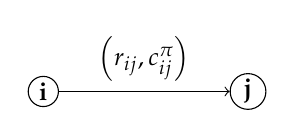
\begin{tikzpicture}[nodes={font=\bf\small}, scale=0.65]
%  \draw [help lines] (-1,-1) grid (8,5);o

\tikzstyle{tasknode}=[%
  draw,
  circle,
  minimum width=0.4,
  inner sep=0.5mm,
]

% nodes
\node [tasknode] (i) at (0, 0) {i};
\node [tasknode] (j) at (4, 0) {j};

\path [draw, ->] (i) -- node[above] {$\left(r_{ij},c_{ij}^{\pi}\right)$} (j);

\end{tikzpicture} 
%%%%%%%%%%%%%%%%%%%%%%%%%%%%%%%%%%%%%%%%%%%

        \caption{Notation: each arc is labelled with residual capacity and reduced cost.} 
        \label{fig:cs-trace:key}
    \end{subfigure}
    \begin{subfigure}[c]{0.5\textwidth}
        %%%%%%%%%%%%%%%%%%%%%%%%%%%%%%%%%%%%%%%%%%%
\begin{tikzpicture}[nodes={font=\bf\small}, scale=0.45]
%  \draw [help lines] (-1,-1) grid (8,5);o

\tikzstyle{mynode}=[%
  draw,
  circle,
  minimum width=0.4,
  inner sep=0.5mm,
]

\tikzstyle{myarc}=[%
  draw,
  arrows={-Triangle[scale=1]},
  line width=1pt,
]

% nodes
\node [mynode] (a) at (0, 4) {A};
\node [mynode] (b) at (4, 8) {B};
\node [mynode] (c) at (4, 0) {C};
\node [mynode] (d) at (8, 4) {D};

% excesses
\node [left=0.5cm] at (0,4.3) {$e_A = 3$}; % A
\node [above=0.6cm] at (4,8) {$e_B = 0$}; % B
\node [below=0.2cm] at (4,0) {$e_C = 0$}; % C
\node [right=0.5cm] at (8,4.3) {$e_D = -3$}; % D

% potentials
\node [left=0.5cm] at (0,3.7) {$\pi_A = 0$}; % A
\node [above=0.15cm] at (4,8) {$\pi_B = 0$}; % B
\node [below=0.65cm] at (4,0) {$\pi_C = 0$}; % C
\node [right=0.5cm] at (8,3.7) {$\pi_D = 0$}; % D

\path [myarc] (a) -- node[above, sloped] {$(2,1)$} (b);
\path [myarc] (a) -- node[below, sloped] {$(3,5)$} (c);
\path [myarc] (b) -- node[right] {$(5,10)$} (c);
\path [myarc] (b) -- node[above, sloped] {$(1,1)$} (d);
\path [myarc] (c) -- node[below, sloped] {$(5,1)$} (d);

\end{tikzpicture} 

        \caption{Initial network. $Q = \left[A\right]$.}
        \label{fig:cs-trace:initial}        
    \end{subfigure}
    \begin{subfigure}[c]{0.5\textwidth}
        %%%%%%%%%%%%%%%%%%%%%%%%%%%%%%%%%%%%%%%%%%%
\begin{tikzpicture}[nodes={font=\bf\small}, scale=0.45]
%  \draw [help lines] (-1,-1) grid (8,5);o

% epsilon=10
% Q=[A]  
% discharge A
% No negative reduced costs: relabel.
% Pi(A) = 0 + 1 + 10 = 11
% Q=[A]

\tikzstyle{mynode}=[%
  draw,
  circle,
  minimum width=0.4,
  inner sep=0.5mm,
]

\tikzstyle{myarc}=[%
  draw,
  arrows={-Triangle[scale=1]},
  line width=1pt,
]

% nodes
\node [mynode] (a) at (0, 4) {A};
\node [mynode] (b) at (4, 8) {B};
\node [mynode] (c) at (4, 0) {C};
\node [mynode] (d) at (8, 4) {D};

% excesses
\node [left=0.55cm] at (0,4.5) {$e_A = 3$}; % A
\node [above=0.6cm] at (4,8) {$e_B = 0$}; % B
\node [below=0.2cm] at (4,0) {$e_C = 0$}; % C
\node [right=0.3cm] at (8,4.5) {$e_D = -3$}; % D

% potentials
\node [left=0.3cm] at (0,3.5) {\color{red} $\pi_A = 11$}; % A
\node [above=0.15cm] at (4,8) {$\pi_B = 0$}; % B
\node [below=0.65cm] at (4,0) {$\pi_C = 0$}; % C
\node [right=0.3cm] at (8,3.5) {$\pi_D = 0$}; % D

\path [myarc] (a) -- node[above, sloped] {\color{red} $(2,-10)$} (b);
\path [myarc] (a) -- node[below, sloped] {\color{red} $(3,-6)$} (c);
\path [myarc] (b) -- node[right] {$(5,1)$} (c);
\path [myarc] (b) -- node[above, sloped] {$(1,10)$} (d);
\path [myarc] (c) -- node[below, sloped] {$(5,1)$} (d);

\end{tikzpicture} 
%%%%%%%%%%%%%%%%%%%%%%%%%%%%%%%%%%%%%%%%%%%

        \caption{$\textproc{Discharge}(A)$: immediately calls $\textproc{Relabel}(A)$ as there are no outgoing arcs with negative reduced cost. $Q$ remains $\left[A\right]$, as $A$ is popped and then immediately pushed again.}
        \label{fig:cs-trace:first}
    \end{subfigure}
    \begin{subfigure}[c]{0.5\textwidth}
        %%%%%%%%%%%%%%%%%%%%%%%%%%%%%%%%%%%%%%%%%%%
\begin{tikzpicture}[nodes={font=\bf\small}, scale=0.45]
%  \draw [help lines] (-1,-1) grid (8,5);o

% epsilon=10
% Q=[A]  
% discharge A
% Push(A,B)  
% Q=[B]
% Push(A,C)
% Q=[B,C]

\tikzstyle{mynode}=[%
  draw,
  circle,
  minimum width=0.4,
  inner sep=0.5mm,
]

\tikzstyle{myarc}=[%
  draw,
  arrows={-Triangle[scale=1]},
  line width=1pt,
]

% nodes
\node [mynode] (a) at (0, 4) {A};
\node [mynode] (b) at (4, 8) {B};
\node [mynode] (c) at (4, 0) {C};
\node [mynode] (d) at (8, 4) {D};

% excesses
\node [left=0.55cm] at (0,4.5) {$e_A = 0$}; % A
\node [above=0.6cm] at (4,8) {$e_B = 2$}; % B
\node [below=0.2cm] at (4,0) {$e_C = 1$}; % C
\node [right=0.3cm] at (8,4.5) {$e_D = -3$}; % D

% potentials
\node [left=0.3cm] at (0,3.5) {$\pi_A = 11$}; % A
\node [above=0.15cm] at (4,8) {$\pi_B = 0$}; % B
\node [below=0.65cm] at (4,0) {$\pi_C = 0$}; % C
\node [right=0.3cm] at (8,3.5) {$\pi_D = 0$}; % D

\path [myarc] (b) -- node[above, sloped] {$(2,10)$} (a);
\path [myarc] (a) -- node[below, sloped] {$(2,-6)$} (c);
\path [myarc] (c) edge[bend right=20, looseness=1] node[above, sloped] {$(1,6)$} (a);
\path [myarc] (b) -- node[right] {$(5,1)$} (c);
\path [myarc] (b) -- node[above, sloped] {$(1,10)$} (d);
\path [myarc] (c) -- node[below, sloped] {$(5,1)$} (d);

\end{tikzpicture} 
%%%%%%%%%%%%%%%%%%%%%%%%%%%%%%%%%%%%%%%%%%%

        \caption{$\textproc{Discharge}(A)$: calls $\textproc{Push}(A,B)$ and $\textproc{Push}(A,C)$, leaving $Q = \left[B,C\right]$.}
        \label{fig:cs-trace:second}        
    \end{subfigure}
    \begin{subfigure}[c]{0.5\textwidth}
        %%%%%%%%%%%%%%%%%%%%%%%%%%%%%%%%%%%%%%%%%%%
\begin{tikzpicture}[nodes={font=\bf\small}, scale=0.45]
%  \draw [help lines] (-1,-1) grid (8,5);o

% epsilon=10
% Q=[B,C]
% discharge B
% relabel B
% Pi(B)=0+1+10=11
% Q=[C,B]

\tikzstyle{mynode}=[%
  draw,
  circle,
  minimum width=0.4,
  inner sep=0.5mm,
]

\tikzstyle{myarc}=[%
  draw,
  arrows={-Triangle[scale=1]},
  line width=1pt,
]

% nodes
\node [mynode] (a) at (0, 4) {A};
\node [mynode] (b) at (4, 8) {B};
\node [mynode] (c) at (4, 0) {C};
\node [mynode] (d) at (8, 4) {D};

% excesses
\node [left=0.75cm] at (0,4.3) {$e_1 = 0$}; % A
\node [above=0.6cm] at (4,8) {$e_2 = 2$}; % B
\node [below=0.2cm] at (4,0) {$e_3 = 1$}; % C
\node [right=0.5cm] at (8,4.3) {$e_4 = -3$}; % D

% potentials
\node [left=0.5cm] at (0,3.7) {$\pi_1 = 11$}; % A
\node [above=0.15cm] at (4,8) {$\pi_2 = 11$}; % B
\node [below=0.65cm] at (4,0) {$\pi_3 = 0$}; % C
\node [right=0.5cm] at (8,3.7) {$\pi_4 = 0$}; % D

\path [myarc] (b) -- node[above, sloped] {$(2,-1)$} (a);
\path [myarc] (a) -- node[below, sloped] {$(2,-6)$} (c);
\path [myarc] (c) edge[bend right=20, looseness=1] node[above, sloped] {$(1,6)$} (a);
\path [myarc] (b) -- node[right] {$(5,-10)$} (c);
\path [myarc] (b) -- node[above, sloped] {$(1,-1)$} (d);
\path [myarc] (c) -- node[below, sloped] {$(5,1)$} (d);

\end{tikzpicture} 
%%%%%%%%%%%%%%%%%%%%%%%%%%%%%%%%%%%%%%%%%%%

        \caption{$\textproc{Discharge}(B)$: immediately calls $\textproc{Relabel}(B)$, leaving $Q = \left[C,B\right]$.}
        \label{fig:cs-trace:third}
    \end{subfigure}
    \begin{subfigure}[c]{0.5\textwidth}
       %%%%%%%%%%%%%%%%%%%%%%%%%%%%%%%%%%%%%%%%%%%
\begin{tikzpicture}[nodes={font=\bf\small}, scale=0.45]
%  \draw [help lines] (-1,-1) grid (8,5);o

% epsilon=10
% Q=[C,B]
% discharge C
% relabel C
% Pi(C) = 0 + 1 + 10 = 11
% Q=[B,C]

\tikzstyle{mynode}=[%
  draw,
  circle,
  minimum width=0.4,
  inner sep=0.5mm,
]

\tikzstyle{myarc}=[%
  draw,
  arrows={-Triangle[scale=1]},
  line width=1pt,
]

% nodes
\node [mynode] (a) at (0, 4) {A};
\node [mynode] (b) at (4, 8) {B};
\node [mynode] (c) at (4, 0) {C};
\node [mynode] (d) at (8, 4) {D};

% excesses
\node [left=0.75cm] at (0,4.3) {$e_1 = 0$}; % A
\node [above=0.6cm] at (4,8) {$e_2 = 2$}; % B
\node [below=0.2cm] at (4,0) {$e_3 = 1$}; % C
\node [right=0.5cm] at (8,4.3) {$e_4 = -3$}; % D

% potentials
\node [left=0.5cm] at (0,3.7) {$\pi_1 = 11$}; % A
\node [above=0.15cm] at (4,8) {$\pi_2 = 11$}; % B
\node [below=0.65cm] at (4,0) {$\pi_3 = 11$}; % C
\node [right=0.5cm] at (8,3.7) {$\pi_4 = 0$}; % D

\path [myarc] (b) -- node[above, sloped] {$(2,-1)$} (a);
\path [myarc] (a) -- node[below, sloped] {$(2,5)$} (c);
\path [myarc] (c) edge[bend right=20, looseness=1] node[above, sloped] {$(1,-5)$} (a);
\path [myarc] (b) -- node[right] {$(5,1)$} (c);
\path [myarc] (b) -- node[above, sloped] {$(1,-1)$} (d);
\path [myarc] (c) -- node[below, sloped] {$(5,-10)$} (d);

\end{tikzpicture} 
%%%%%%%%%%%%%%%%%%%%%%%%%%%%%%%%%%%%%%%%%%%

        \caption{$\textproc{Discharge}(C)$: immediately calls $\textproc{Relabel}(C)$, leaving $Q = \left[B,C\right]$.}
        \label{fig:cs-trace:fourth}
    \end{subfigure}
    \caption[Cost scaling in action with FIFO vertex queue]{Partial trace of FIFO \textproc{Refine} from \cref{algo:cost-scaling-first-active-refine}, depicting the residual network after each call to \textproc{Discharge}. Each node $i$ is labelled with its excess $e_i$ and potential $\pi_i$. $\epsilon$ is taken to be $10$, as would be the case on the first call to \textproc{Refine} from \cref{algo:cost-scaling} (note the maximum cost $C$ in the network is 10.)}
    \label{fig:cs-trace}
\end{figure}

\begin{algorithm}
\begin{algorithmic}[1]
    \Function{Refine}{$\mathbf{x}$,$\boldsymbol{\pi}$,$\epsilon$}
        \State initialisation as in lines 2-4 of \cref{algo:cost-scaling-generic-refine}
        \Let{$Q$}{$\left[s \in V \::\: e_s > 0\right]$} \Comment{$Q$ is a queue of excess vertices}
        \While{$Q$ not empty}
            \State pop head of $Q$ into $s$
            \State \Call{Discharge}{$s$,$\epsilon$} \Comment{May add vertices to $Q$}
            \If{\textproc{Relabel} called by \textproc{Discharge}}
                \State add $s$ to rear of $Q$
                \Break
            \EndIf
        \EndWhile
    \EndFunction
\end{algorithmic}
\caption{Cost scaling: FIFO \textproc{Refine} routine}
\label{algo:cost-scaling-first-active-refine}
\end{algorithm}

\Cref{algo:cost-scaling-first-active-refine} maintains a first-in-first-out (FIFO) queue $Q$ of excess vertices (see \cref{sec:prep-flow-pseudo}). The initial order of vertices in the queue is arbitrary. At each iteration, an excess vertex $s$ is removed from the head of the queue, and \emph{discharged} by applying a sequence of \textproc{Push} and \textproc{Relabel} operations (described below). During execution of the algorithm, new vertices may gain an excess; in this case, they are added to the rear of $Q$.

\begin{algorithm}
\begin{algorithmic}[1]
    \Require{$e_s > 0$}
    \Function{Discharge}{$s$,$\epsilon$}
        \Repeat
            \State \Call{PushOrRelabel}{$s$,$\epsilon$}
        \Until $e_s \leq 0$
    \EndFunction
    \stepcounter{algorithmicH}
    \setcounter{ALG@line}{0}
    \Statex
    \Require{$e_s > 0$}
    \Function{PushOrRelabel}{$s$,$\epsilon$}
        \State let $(i,j)$ be the current arc of $s$
        \If{$(i,j) \in E_\mathbf{x}$ and $c_{ij}^{\boldsymbol{\pi}} < 0$} \Call{Push}{$i$,$j$}
        \Else
            \If{$(i,j)$ last arc on the adjacency list for $s$}
                \State \Call{Relabel}{$s$}
                \Let{current arc}{first arc in adjacency list}
            \Else
                \Let{current arc}{next arc in adjacency list}
            \EndIf
        \EndIf
    \EndFunction
\end{algorithmic}
\caption{Cost scaling: \textproc{Discharge} and helper routine \textproc{PushOrRelabel}}
\label{algo:cost-scaling-discharge}
\end{algorithm}

$\textproc{Discharge}(s)$ is described in \cref{algo:cost-scaling-discharge}. It may be applied to any excess vertex, and performs a sequence of push operations until $e_s = 0$ or \textproc{Relabel} is called. For each vertex $i \in V$, an adjacency list is maintained, in a fixed (but arbitrary) order. The helper routine \textproc{PushOrRelabel} walks over this adjacency list, performing \textproc{Push} operations when possible. When the end of this adjacency list is reached, no further \textproc{Push} operations can be performed, and \textproc{Relabel} is invoked.

Note any new excess vertices generated during execution of the algorithm must be added to the rear of $Q$. $\textproc{Push}(i,j)$ may make $j$ an excess vertex: \cref{algo:cost-scaling-operations} must be modified to check for this case. The code for \textproc{Refine} in \cref{algo:cost-scaling-generic-refine} must also be updated. \textproc{Refine} pops $s$ from $Q$ and then calls \textproc{Discharge}. If \textproc{Relabel} is called by \textproc{Discharge}, $s$ will still be an active vertex when \textproc{Discharge} returns, and must be added back to the queue $Q$.

\Cref{fig:cs-trace} illustrates the operation of FIFO \textproc{Refine}, showing how each call to \textproc{Discharge} modifies the potentials $\mathbf{\pi}$ and flow $\mathbf{x}$ on a simple network.

\begin{thm} \label{thm:cost-scaling-first-active-complexity}
The algorithm with FIFO refine has a running time of $O(n^2m \lg (nC))$.
\end{thm}
\begin{proof}
See Goldberg and Tarjan~\cite[theorem~6.2]{Goldberg:1990}.
\end{proof}

\begin{remark}
In fact, this complexity bound holds for any refine routine which repeatedly applies \textproc{PushOrRelabel}. However, it has been conjectured by Goldberg that the FIFO ordering of vertices in this variant results in a tighter bound of $O(n^3 \lg (nC))$. Proving or disproving this assertion is an open research problem.\\
\end{remark} 

\begin{remark}
On flow scheduling networks, $m = O(n)$ by \cref{lemma:network-num-arcs}, so the bound is trivially $O(n^3 \lg (nC))$ in any case.
\end{remark}

\subsubsection{Wave refine} \label{sec:impl-cs-impl-wave}

\begin{algorithm}
\begin{algorithmic}[1]
    \Function{Refine}{$\mathbf{x}$,$\boldsymbol{\pi}$,$\epsilon$}
    \State initialisation as in lines 2-4 of \label{algo:cost-scaling-wave-refine:initialisation} \cref{algo:cost-scaling-generic-refine}
    \Let{$L$}{list of vertices in $V$} \Comment{order of vertices is arbitrary}
    \Repeat
        \For{each vertex $i$ in list $L$}
            \If{$e_i > 0$}
                \State \Call{Discharge}{$i$,$\epsilon$}
                \If{\textproc{Relabel} called by \textproc{Discharge}}
                    \State move $i$ to front of $L$
                \EndIf
            \EndIf
        \EndFor
    \Until{no excess vertex encountered in \textbf{for} loop}
    \EndFunction
\end{algorithmic}
\caption{Cost scaling: wave \textproc{Refine} routine}
\label{algo:cost-scaling-wave-refine}
\end{algorithm}

\Cref{algo:cost-scaling-wave-refine} describes an approach which can be proved to achieve the $O(n^3 \lg (nC))$ bound on any flow network. The method maintains a list $L$ of all vertices in the network, rather than the queue $Q$ maintained by the FIFO method. The algorithm preserves the invariant that $L$ is topologically ordered with respect to the \emph{admissible graph}: the subgraph of the residual network containing only arcs with negative reduced cost.

Initially, $L$ contains vertices in arbitrary order. But the admissible graph is empty after \cref{algo:cost-scaling-wave-refine:initialisation} of \cref{algo:cost-scaling-wave-refine}, since \crefrange{algo:cost-scaling-generic-refine:start-init}{algo:cost-scaling-generic-refine:end-init} of \cref{algo:cost-scaling-generic-refine} saturate any negative reduced cost arcs, making them drop out of the residual network. Thus, $L$ is trivially topologically ordered.

\textproc{Push} operations cannot create admissible arcs, and so preserve the topological ordering. An operation $\textproc{Relabel}(s)$ can create admissible arcs. However, there are guaranteed to be no admissible arcs entering $s$ immediately after the operation~\cite[lemma~6.5]{Goldberg:1987}. Moving $s$ to the beginning of $L$ therefore ensures a topological ordering is maintained.\\

\begin{thm} \label{thm:cost-scaling-wave-complexity}
The algorithm with wave refine has a running time of $O(n^3 \lg (nC))$.
\end{thm}
\begin{proof}
Using the invariant that $L$ is topologically ordered, it is possible to prove an $O(n^2)$ bound on the number of passes over the vertex list~\cite[lemma~7.3]{Goldberg:1987}. An $O(n^3)$ bound on the running time of the wave \textproc{Refine} routine can be shown as a corollary of this~\cite[theorem~7.4]{Goldberg:1987}. The result follows by \cref{lemma:cost-scaling-overall-algorithm}.
\end{proof}

\subsection{Heuristics}

So far, this dissertation has only considered means to improve the theoretical performance of cost scaling. Considerable research effort has gone into improving its practical performance by means of \emph{heuristics} that guide the actions of the algorithm~\cite{Goldberg:1997}.

I decided not to implement any heuristics. The heuristics are already well-studied: implementing them would not have produced any new insight, and would have diverted considerable development time from other efforts. I judged that it was better to keep my implementation simple, allowing me to rapidly explore fundamentally different approaches. However, for the sake of completeness I have summarised the heuristics in \cref{appendix:impl-csheuristics}.

% Optimisations: changing scaling factor, maintaining integrality, wave vs sequential
% Optimisations may be better left for evaluation? If you do want to include it here, should merge it into heuristics with a section e.g. Improving performance

\section{Approximation algorithms} \label{sec:impl-approx}

% PROOFREAD - Intro: 1 major edits, 2 minor edits

Feasible solutions to flow scheduling networks correspond to scheduling assignments. A solution's cost indicates the degree to which the assignment meets the scheduler's policy goals. The algorithms considered so far find \emph{minimal} cost flows, producing scheduling assignments which \emph{maximise} the policy objectives.

Finding the best solution may take some time, yet minimising scheduling latency is itself important (see \cref{sec:prep-scheduling}). I develop an approximate solution method, allowing the trade-off between accuracy and speed to be chosen explicitly.

% It may be possible to find an \emph{approximate} solution -- a flow with low, albeit not minimal, cost -- faster than an optimal solution. Whole-system performance may improve due to the reduction in scheduling latency, in spite of a less-than-optimal allocation of tasks.
%However, finding the best solution may take some time, yet minimising scheduling latency is itself an important objective (see \cref{sec:prep-scheduling}). It is wasteful for machines to run idle, waiting for tasks to be scheduled; moreover, interactive applications cannot tolerate high scheduling delays. I develop an \emph{approximate} solver, allowing the trade-off between scheduling accuracy and speed to be chosen explicitly.

I believe this is the first study of approximation algorithms for the minimum-cost flow problem. There is some prior work on finding approximate solutions for the related NP-complete problems of multi-commodity flows~\cite{Garg:2007} and dynamic flows~\cite{Hoppe:1994}. These techniques are of limited applicability to minimum-cost flow problems\footnotemark, however, and Hapi uses entirely different methods for approximation.
\footnotetext{For example, approximation methods for multi-commodity flow problems often work by solving many single-commodity flow problems. Obviously this reduction method does not help when the problem is already single-commodity.}

\subsection{Choice of algorithms} \label{sec:impl-approx-choice}

% PROOFREAD - 1 minor edits.
The solution returned by an approximate algorithm must be \emph{feasible}, although it need not be \emph{optimal}. Of the algorithms considered in sections \ref{sec:impl-cycle-cancelling} to \ref{sec:impl-cost-scaling}, only cycle cancelling and cost scaling maintain feasibility as an invariant\footnotemark.
\footnotetext{Successive shortest path and relaxation, by contrast, operate on a pseudoflow and maintain optimality as an invariant.}

Both cycle cancelling and cost scaling find successive approximations to an optimal solution, and so can readily be adapted to find approximate solutions. In cycle cancelling, the cost of the solution monotonically decreases after each iteration (shown in the proof of \cref{lemma:cycle-cancelling-termination}). However, a large decrease in the cost of the solution may occur at \emph{any} point in the algorithm's execution.

By contrast, in cost scaling the error bound $\epsilon$ undergoes exponential decay\footnotemark, reaching a small value many iterations before the algorithm would normally terminate. It will therefore produce a better approximation than cycle cancelling. Cost scaling is also considerably faster than cycle cancelling, making it the clear choice for an approximate solver.
\footnotetext{The solution cost \emph{tends} to also undergo exponential decay. However, this is not guaranteed: the error bound is not tight, and the cost on occasion may even increase.}

\subsection{Adapting cost scaling} \label{sec:impl-approx-adaptions}

% PROOFREAD - 1 major edits.
Cost scaling finds successive $\epsilon$-optimal solutions, where $\epsilon$ is decreased by a constant factor $\alpha$ after every iteration (see \cref{algo:cost-scaling}). It terminates when $\epsilon < 1/n$, at which point the solution is optimal by \cref{thm:epsilon-optimality-optimal}. Relaxing this terminating condition produces an approximate solver.

Ideally, it would be possible to specify a bound on the relative error of the solution: for example, terminating once the error is smaller than 1\%. Unfortunately, computing the relative error requires knowing the minimum cost, which can only be determined by finding an optimal solution.

It is possible to derive a bound on the absolute error of the solution, in terms of $\epsilon$. Unfortunately, the bound is of limited practical use. \Cref{defn:epsilon-optimality} of $\epsilon$-optimality has the simple corollary that:

\[\epsilon = \max_{(i,j) \in E_\mathbf{x}} -c_{ij}^{\boldsymbol{\pi}}\]

$\epsilon$ therefore depends on the `worst' arc in the residual network: i.e.\ the one with the most negative reduced cost. If every arc were to attain this worst case, the error could be large even for small values of $\epsilon$. But in practice, this does not occur. The bound therefore tends to significantly overestimate the solution error.

As accurate analytic bounds on the error are not available, I had to develop heuristic terminating conditions. These are the focus of the rest of this section.

% N.B. Commented out as never evaluated, and it's kind of a stupid heuristic anyway.
%\subsubsection{$\epsilon$ threshold}
%
%In this heuristic, the algorithm terminates as soon as $\epsilon$ drops below some fixed threshold. Note that setting the threshold to $1/n$ recovers the original algorithm.
%
%More sophisticated heuristics are expected to outperform this technique. However, as the simplest possible approach, it serves as a natural baseline for evaluation.

\subsubsection{Cost convergence}

\begin{figure}
    \centering
    \includegraphics{app/quincy_medium_over_time_2col}
    \caption[Successive approximations to an optimal solution.]{Successive approximations to an optimal solution. Each iteration of cost scaling is marked by a point on the graph. The spacing between points on the $x$-axis indicate the time taken by \textproc{Refine}. This varies throughout execution of the algorithm, but does not show any trend: \textproc{Refine} runs for a similar length of time immediately before optimality as for the first iteration. Note that the $y$-axis, representing solution cost, is on a log scale. The results are for a scheduling flow network from the dataset described in \cref{sec:eval-approx-flow-scheduling}.}
    \label{fig:app-cost-over-time}
\end{figure}

The first few iterations of cost scaling tend to produce large reductions in the cost. When the solution is nearly optimal, the change in cost between successive iterations is typically small. This is illustrated in \cref{fig:app-cost-over-time}, which shows cost scaling running on a scheduling flow network. 

Cost convergence exploits this property, by measuring the difference between the cost after successive iterations. If the cost changes by a factor less than some threshold $t$, the algorithm terminates.

%On some flow networks, cost scaling hits a brief `plateau', before continuing to make significant cost reductions. My implementation can optionally consider multiple prior iterations, terminating only when the cost change is below the threshold in the last $k \geq 1$ iterations, to combat this.

\subsubsection{Task migration convergence}

Cost convergence is a general approach, applicable to any class of flow network. By contrast, this heuristic exploits the nature of flow scheduling. Vertices are labelled as representing either a task, machine or other entity. Task assignments are computed from the flow (see \cref{sec:prep-flow-scheduling}), and the number of changes from the last iteration is measured. The algorithm terminates when this drops below a threshold $t$.

% Extensions: hybrid schemes? Error bounds based on arcs being fixed?

\section{Incremental algorithms} \label{sec:impl-incremental}

\begin{figure}
    \centering
    \begin{subfigure}[c]{\textwidth}
        \centering
        %%%%%%%%%%%%%%%%%%%%%%%%%%%%%%%%%%%%%%%%%%%
\begin{tikzpicture}[nodes={font=\bf\small}, scale=0.65]
%  \draw [help lines] (-1,-1) grid (8,5);o

\tikzstyle{tasknode}=[%
  draw,
  circle,
  minimum width=0.4,
  inner sep=0.5mm,
]

% T_0,0
\node [tasknode, black!70!green] (t00) at (0,6.5) {T$_0^0$};
% T_0,1
\node [tasknode, black!70!green] (t01) at (0,4.5) {T$_1^0$};

% X
\node [draw, rectangle, brown] (x) at (5.0,3.5) {X};

% M_0 & M_1
\node [draw, rectangle, blue] (m0) at (10.0,6.5) {M$_0$};
\node [draw, rectangle, blue] (m1) at (10.0,4.5) {M$_1$};
\node [draw, rectangle, blue] (m2) at (10.0,2.5) {M$_2$};

% sink
\node [draw, regular polygon, regular polygon sides=6] (s) at (12, 3.5) {S};

% U_0
\node [draw, rectangle, red] (u0) at (5.0,7.0) {U$^0$};

% Tasks to X
\path [draw, ->] (t00) -- node[below, sloped] {1} (x);
\path [draw, ->] (t01) -- node[below, sloped] {1} (x);

% Tasks to U_i
\path [draw, ->] (t00) -- node[above, sloped] {5} (u0);
\path [draw, ->] (t01) -- node[above, sloped] {5} (u0);

% X to machines
\path [draw, ->] (x) -- node[below, sloped] {} (m0);
\path [draw, ->] (x) -- node[below, sloped] {} (m1);
\path [draw, ->] (x) -- node[below, sloped] {} (m2);

% Machines to sink
\path [draw, ->, red] (m0) -- node[above, sloped] {} (s);
\path [draw, ->, red] (m1) -- node[below, sloped] {} (s);
\path [draw, ->] (m2) -- node[below, sloped] {} (s);

% U_i to sink
\begin{scope}[decoration={post length=4pt},rounded corners=4mm]
  \path [draw, ->] (u0) -- ++(1.5,0.5) -- node[below, sloped] {} ++(6,0) -- ++(1,-0.5) -- (s);
\end{scope}

% running tasks
\path [draw, ->, dotted, red] (t00) edge[out=-30, in=180, looseness=1] node[above, sloped] {1} (m0);
\path [draw, ->, dotted, red] (t01) edge[out=15, in=180, looseness=1] node[above, sloped] {1} (m1);

\end{tikzpicture} 
%%%%%%%%%%%%%%%%%%%%%%%%%%%%%%%%%%%%%%%%%%%

        \vspace*{1em}        
        \caption{The initial network, showing tasks $\mathbf{T}_0^0$ and $\mathbf{T}_1^0$ running on $\mathbf{M}_0$ and $\mathbf{M}_1$ respectively.}
        \vspace*{2em}
    \end{subfigure}
    \begin{subfigure}[c]{\textwidth}
        \centering
        %%%%%%%%%%%%%%%%%%%%%%%%%%%%%%%%%%%%%%%%%%%
\begin{tikzpicture}[nodes={font=\bf\small}, scale=0.65]
%  \draw [help lines] (-1,-1) grid (8,5);o

\tikzstyle{tasknode}=[%
  draw,
  circle,
  minimum width=0.4,
  inner sep=0.5mm,
]

% T_0,0
\node [tasknode, green] (t00) at (0,6.5) {T$_0^0$};
% T_0,1
\node [tasknode, green] (t01) at (0,4.5) {T$_1^0$};

% T_1,0
\node [tasknode, green] (t10) at (0,1.5) {T$_0^1$};

% X
\node [draw, rectangle, brown] (x) at (5.0,3.5) {X};

% M_0 & M_1
\node [draw, rectangle, blue] (m0) at (10.0,6.5) {M$_0$};
\node [draw, rectangle, blue] (m1) at (10.0,4.5) {M$_1$};
\node [draw, rectangle, blue] (m2) at (10.0,2.5) {M$_2$};

% sink
\node [draw, regular polygon, regular polygon sides=6] (s) at (12, 3.5) {S};

% U_0
\node [draw, rectangle, red] (u0) at (6.0,7.5) {U$^0$};
% U_1
\node [draw, rectangle, red] (u1) at (6.0,0.5) {U$^1$};

% Tasks to X
\path [draw, ->] (t00) -- node[above, sloped] {3} (x);
\path [draw, ->] (t01) -- node[below, sloped] {3} (x);
\path [draw, ->, red] (t10) -- node[below, sloped] {2} (x);

% Tasks to U_i
\path [draw, ->] (t00) -- node[above, sloped] {10} (u0);
\path [draw, ->] (t01) -- node[above, sloped] {10} (u0);
\path [draw, ->] (t10) -- node[below, sloped] {5} (u1);

% X to machines
\path [draw, ->] (x) -- node[below, sloped] {} (m0);
\path [draw, ->] (x) -- node[below, sloped] {} (m1);
\path [draw, ->, red] (x) -- node[below, sloped] {} (m2);

% Machines to sink
\path [draw, ->, red] (m0) -- node[above, sloped, red] {} (s);
\path [draw, ->, red] (m1) -- node[below, sloped, red] {} (s);
\path [draw, ->, red] (m2) -- node[below, sloped] {} (s);

% U_i to sink
\begin{scope}[decoration={post length=4pt},rounded corners=4mm]
  \path [draw, ->] (u0) -- ++(1.5,0.5) -- node[below, sloped] {} ++(4,0)  -- (s);
  \path [draw, ->] (u1) -- ++(1.5,-0.5) -- node[above, sloped] {} ++(4,0) -- (s);
\end{scope}

% running task
\path [draw, ->, dotted, red] (t00) edge[out=-20, in=190, looseness=1] node[above, sloped] {1} (m0);
\path [draw, ->, dotted, red] (t01) edge[out=0, in=170, looseness=1] node[above, sloped] {2} (m1);

\end{tikzpicture} 
%%%%%%%%%%%%%%%%%%%%%%%%%%%%%%%%%%%%%%%%%%%

        \vspace*{1em}
        \caption{A job is submitted, consisting of a single task $\mathbf{T}^1_0$. It has no preference arcs, so its flow drains through $\mathbf{X}$ and into the idle machine $\mathbf{M}_2$.}
        \label{fig:inc-network:new-job-idle}        
        \vspace*{2em}
    \end{subfigure}
    \begin{subfigure}[c]{\textwidth}
        \centering
        %%%%%%%%%%%%%%%%%%%%%%%%%%%%%%%%%%%%%%%%%%%
\begin{tikzpicture}[nodes={font=\bf\small}, scale=0.65]
%  \draw [help lines] (-1,-1) grid (8,5);o

\tikzstyle{tasknode}=[%
  draw,
  circle,
  minimum width=0.4,
  inner sep=0.5mm,
]

% T_0,0
\node [tasknode, black!70!green] (t00) at (0,6.5) {T$_0^0$};
% T_0,1
\node [tasknode, black!70!green] (t01) at (0,4.5) {T$_1^0$};

% T_1,0
\node [tasknode, black!70!green] (t10) at (0,1.5) {T$_0^1$};

% X
\node [draw, rectangle, brown] (x) at (5.0,3.5) {X};

% M_0 & M_1
\node [draw, rectangle, blue] (m0) at (10.0,6.5) {M$_0$};
\node [draw, rectangle, blue] (m1) at (10.0,4.5) {M$_1$};
\node [draw, rectangle, blue] (m2) at (10.0,2.5) {M$_2$};

% sink
\node [draw, regular polygon, regular polygon sides=6] (s) at (12, 3.5) {S};

% U_0
\node [draw, rectangle, red] (u0) at (6.0,7.5) {U$^0$};
% U_1
\node [draw, rectangle, red] (u1) at (6.0,0.5) {U$^1$};

% Tasks to X
\path [draw, ->] (t00) -- node[above, sloped] {3} (x);
\path [draw, ->, red] (t01) -- node[below, sloped] {3} (x);
\path [draw, ->] (t10) -- node[below, sloped] {10} (x);

% Tasks to U_i
\path [draw, ->] (t00) -- node[above, sloped] {10} (u0);
\path [draw, ->] (t01) -- node[above, sloped] {10} (u0);
\path [draw, ->] (t10) -- node[below, sloped] {5} (u1);

% X to machines
\path [draw, ->] (x) -- node[below, sloped] {} (m0);
\path [draw, ->] (x) -- node[below, sloped] {} (m1);
\path [draw, ->, red] (x) -- node[below, sloped] {} (m2);

% Machines to sink
\path [draw, ->, red] (m0) -- node[above, sloped, red] {} (s);
\path [draw, ->, red] (m1) -- node[below, sloped, red] {} (s);
\path [draw, ->, red] (m2) -- node[below, sloped] {} (s);

% U_i to sink
\begin{scope}[decoration={post length=4pt},rounded corners=4mm]
  \path [draw, ->] (u0) -- ++(1.5,0.5) -- node[below, sloped] {} ++(4,0)  -- (s);
  \path [draw, ->] (u1) -- ++(1.5,-0.5) -- node[above, sloped] {} ++(4,0) -- (s);
\end{scope}

% running task
\path [draw, ->, dotted, red] (t00) edge[out=-20, in=190, looseness=1] node[above, sloped] {1} (m0);
\path [draw, ->, dotted] (t01) edge[out=0, in=170, looseness=1] node[above, sloped] {2} (m1);

% preference arc
\path [draw, ->, dashed, red] (t10) edge[out=-5, in=200, looseness=1] node[above, sloped] {1} (m1);

\end{tikzpicture} 
%%%%%%%%%%%%%%%%%%%%%%%%%%%%%%%%%%%%%%%%%%%

        \vspace*{1em}        
        \caption{An alternative to (b), where the task has a strong preference for running on machine $\mathbf{M}_1$, which is busy executing task $\mathbf{T}_1^0$. The cost of the running arc $\mathbf{T}_1^0 \to \mathbf{M}_1$ is lower than the cost of $\mathbf{T}_1^0 \to \mathbf{X}$, as the task is partially complete (see \cref{appendix:flow-scheduling:costs}). Nevertheless, the cheapest option is to \emph{migrate} $\mathbf{T}_1^0$ to $\mathbf{M}_2$, satisfying $\mathbf{T}_0^1$'s strong preference.}
    \end{subfigure}
    \caption[An incremental change to a scheduling flow network]{(b) and (c) show the result of incremental changes to the original network (a). Arcs are labelled with their cost; any unlabelled arc has a cost of zero. The optimal solution is shown by highlighting the arcs which carry flow in {\color{red} red}. Dotted lines represent \textbf{running arcs}, dashed lines \textbf{preference arcs} (see \cref{sec:prep-flow-scheduling}).}
    \label{fig:inc-network}
\end{figure}

% PROOFREAD: 1 minor edits, 2 minor edits

% FIGURE: Sequence of flow graphs, showing small change?
Flow scheduling systems produce a sequence of closely related flow networks. Each new network in the sequence is generated in response to cluster events. \Cref{fig:inc-network} gives an example of the changes triggered by task submission, one of the most common events. Other events include task completion, machine addition and removal.

These events cause localised changes to the flow network. Consequently, the optimal flow tends to remain mostly the same. My method of \emph{incremental} solution is designed to exploit this. The algorithm reuses the solution for the old flow network, \emph{reoptimising} to produce an answer for the new network. This approach proved to be extremely successful, producing a factor of $14.5\times$ speedup in my tests (see \cref{sec:eval-incremental}). I believe my implementation is the first of its kind: there is certainly no mention of this method in the literature.

Flow scheduling is ideally suited to an incremental solution method. However, the approach is much less compelling for traditional applications of flow networks: this may go some way to explaining the lack of prior work. As previously mentioned, most network changes in flow scheduling are small. This alone does not make the problem easy: reoptimising after even a single change is, in general, as hard as solving the problem from scratch\footnotemark. Informally, the problem is that since the optimisation problem is global, an update in one region of the network may trigger a cascading sequence of changes in the optimal flow for distant regions.
\footnotetext{To see this, consider two networks $A$ and $B$. WLOG, assume they each have a single supply vertex $s_x$ and demand vertex $t_x$ for $x \in {A,B}$. Remove the supply and demand at those vertices, introducing new supply and demand vertices $s$ and $t$. Add arcs $s\to s_x$ with capacity $b_{s_x}$, and $t_x \to t$ with capacity $-b_{t_x}$, for $x \in {A,B}$. Let $C$ be a cost larger than the cost of any flow in networks $A$ or $B$; set the cost of $s \to s_A$ to $C$ and $s \to s_B$ to $2C$. The resulting network is effectively equivalent to just network $A$. Dropping the cost on $s \to S_B$ from $2C$ to $0$ makes the resulting network effectively equivalent to $B$. Solving this incremental change is thus as hard as solving the entire network $B$.}

Crucially, however, scheduling policies are designed to produce stable assignments of tasks to machines. Preempting a task is an expensive operation, which should be performed sparingly. Consequently, the cost model for any viable scheduling policy naturally avoids frequent changes to the optimal flow. This is precisely the property required for incremental solvers to perform well.

I describe the sources I drew on to develop my incremental solver in the next section, \cref{sec:impl-incremental-related-work}. Following this, I discuss my approach to building such a solver in \cref{sec:impl-incremental-architecture}. After this background, I evaluate the suitability of different flow algorithms to the incremental problem in \cref{sec:impl-incremental-choice}. Following this, \cref{sec:impl-incremental-impl} provides details of the solvers I implemented.

\subsection{Related work} \label{sec:impl-incremental-related-work}
The Quincy paper highlighted incremental solvers as an area for further research, sparking my interest in such an approach~\cite[\S6.5]{Isard:2007}. There has been some study of reoptimisation and sensitivity analysis on flow networks, which are related to the incremental problem, although these areas have received comparatively little attention. I survey the existing work below.

Amini and Barr published a comprehensive empirical evaluation of reoptimisation algorithms in 1993~\cite{Amini:1993}. However, the study tested algorithms such as the out-of-kilter method, now long obsolete. Moreover, the largest network studied had only 1,500 vertices, orders of magnitude smaller than the ones considered in this project. 

The most recent work is a computational study of algorithms for reoptimisation after arc cost changes, published by Frangioni and Manca in 2006~\cite{Frangioni:2006}. Although now almost a decade old, the algorithms evaluated are still in contemporary use. However, the results of the study may not generalise to flow scheduling, where any parameter -- not just arc costs -- can change. 

Sensitivity analysis on flow networks seeks to determine how uncertainty in network parameters causes uncertainty in the optimal solution~\cite[\S9.11]{Ahuja:1993}. In scientific applications, this may be used to test the robustness of a flow model. Small changes in the input should produce similarly small changes in the output: otherwise, the model is too sensitive to measurement error. Although the goals of sensitivity analysis are considerably different to those of an incremental solver, some of the underlying techniques can be adapted.

\subsection{Architecture of an incremental algorithm} \label{sec:impl-incremental-architecture}

Previous sections in this chapter described the implementation of pre-existing algorithms. These are designed to solve the minimum-cost flow problem ``from scratch'': finding an optimal solution without the benefit of any existing state. An obvious incremental approach is to simply rerun one of these algorithms on the updated network, using the previous state as a starting point.

This does not quite work, however: most flow algorithms maintain an invariant on the state of the solver during intermediate computations. After a network update, this invariant may fail to hold. When the invariant is a precondition for the algorithm, as in relaxation, reoptimisation might fail entirely. In other algorithms, such as cost scaling, the invariant is used only to prove complexity bounds. Reoptimisation will succeed, but may run slower than expected.

Consequently, I adopt a three-step approach for my incremental algorithm:

\begin{enumerate}
    \item Receive changes to the flow network, updating any internal data structures.
    \item Manipulate the saved state, to satisfy the invariant under the updated network.
    \item Run the algorithm to reoptimise.
\end{enumerate}

In practice, implementation of this approach is considerably more challenging than suggested by this summary. Step 1 superficially appears trivial, but many graph data structures cannot be efficiently modified. Considerable research effort has gone into devising \emph{dynamic} data structures to resolve this problem~\cite{Tarjan:1983,Eppstein:1996}. In addition to the network itself, many algorithms rely on auxiliary data structures\footnotemark, which must also be updated.
\footnotetext{For example, many algorithms maintain a set of excess vertices to improve performance.}

Step 2 varies considerably between algorithms, and is discussed in \cref{sec:impl-incremental-impl}. Somewhat ironically, step 3 is the simplest, with the core of the algorithm remaining mostly unmodified. Since step 2 ensures that the invariant holds, the optimisation procedure can be run as usual after disabling any initialisation code.

\subsection{Choice of algorithms} \label{sec:impl-incremental-choice}
The approach suggested above could be applied to any flow algorithm considered in this dissertation. In this section, I consider which algorithms are most suited to operating incrementally. I start with cost scaling, which has excellent performance on the from scratch problem (see \cref{sec:impl-cost-scaling}). Next, I consider successive shortest path and relaxation (see \cref{sec:impl-ssp} and \cref{sec:impl-relax}). I do not discuss cycle cancelling, as it is considerably slower than the other algorithms.

\subsubsection{Cost scaling} 
%WORDCOUNT: Incremental choice of algorithm -- could make cuts to cost scaling
Despite excellent performance on the full problem, Goldberg's cost scaling algorithm fares poorly on the incremental problem. 

Cost scaling maintains the invariant that $\mathbf{x}$ is a feasible flow and $\left(\mathbf{x},\boldsymbol{\pi}\right)$ is $\epsilon$-optimal. This invariant is not required for correctness, but is needed for proofs of its complexity.

The starting state may be neither feasible nor optimal on the new network. To satisfy the invariant, feasibility must first be restored, such as by running a max-flow algorithm\footnotemark, which will tend to make the flow less optimal.
\footnotetext{In fact, it is perfectly legitimate to skip this stage and run \textproc{Refine} directly, which will also restore feasibility. However, the analysis is clearer when considering these stages separately.}

Next, the value of $\epsilon$ for which $\left(\mathbf{x},\boldsymbol{\pi}\right)$ is $\epsilon$-optimal must be calculated. This can be computed by a single pass over the arcs in the residual network. Alternatively, the potential refinement heuristic described in \cref{appendix:impl-csheuristics-potential-refinement} could be used: this might find a smaller value of $\epsilon$ by updating the potentials $\boldsymbol{\pi}$.

% I'm not sure that restoring feasibility does break $\epsilon$-optimality. We can just invoke Refine on the non-feasible flow, that's fine I think.
The key problem is that $\epsilon$ may be very large even after a small update. Recall that $\epsilon$-optimality (see \cref{defn:epsilon-optimality}) is defined as a property satisfied by \emph{every} arc. $\epsilon$ is thus a measure of the \emph{maximum} error in the solution. An update as simple as changing the cost on a single arc can make $\epsilon$ large, even though the rest of the network remains $0$-optimal. Since $\epsilon$ often ends up close (in logarithmic terms) to its starting value $C$, the algorithm performs almost as many iterations of \textproc{Refine} as it would in the full case.
% Below is good, but wordcount.
% Furthermore, there is no reason to hope the iterations will complete any faster than usual. Although \textproc{Refine} maintains $\epsilon$-optimality, it can make previously optimised segments of the network \emph{less} optimal (up to the bound of $\epsilon$), effectively creating more work for future iterations.

%WONTFIX: Would be interesting to try and model the performance of CS2. Simple approach which could work: assume new epsilon is ~U[0,C], what is the mean and variance of log_2 (C/epsilon)?
The computational study of cost reoptimisation by Frangioni and Manca~\cite{Frangioni:2006} supports my assertion. Whereas other algorithms enjoyed speedups of $20\times$ or more, cost scaling had only a $2\times$ speedup. Moreover, its performance was unpredictable, varying considerably even within networks of the same class.

\subsubsection{Successive shortest path and relaxation}

Both the successive shortest path and relaxation algorithm work by sending flow along \emph{augmenting paths}. These paths start at an excess vertex, and reach an excess vertex traversing only arcs of zero or negative reduced cost. Although the two algorithms differ considerably, they have similar incremental properties. In particular, note they both maintain the invariant that $\left(\mathbf{x},\boldsymbol{\pi}\right)$ satisfies reduced-cost optimality conditions, seeking to successively improve the feasibility of $\mathbf{x}$\footnotemark.
\footnotetext{This is most clear in the successive shortest path algorithm, which improves the feasibility of $\mathbf{x}$ on every iteration. It is not strictly speaking the case for the relaxation algorithm, since the the \textproc{UpdatePotentials} operation may make the flow \emph{less} feasible. But, indirectly, \textproc{UpdatePotentials} is still working towards feasibility since it allows for more \textproc{AugmentFlow} operations to take place.}

Changes to the network can violate reduced cost optimality, but the pseudoflow can be modified inexpensively to maintain optimality (see \cref{sec:impl-incremental-maintaining-rc} for my method). The algorithm can then be run as usual to reoptimise, restoring feasibility. This takes time proportional to the reduction in feasibility of the solution caused by the updates\footnotemark. This is a very desirable property for flow scheduling, where most changes will only impact the feasibility of a small region of the network.
\footnotetext{Note that the feasibility may be reduced directly and indirectly. Direct decreases in feasibility occur as an immediate consequence of a network update: for example, adding a new source and sink vertex. The feasibility may also be compromised indirectly: the operations needed to maintain reduced cost optimality might require pushing flows along arcs, resulting in excesses or deficits at vertices.}

The relaxation algorithm is evaluated empirically in the study by Frangioni and Manca. As I discussed in \cref{sec:impl-relax}, the practical performance characteristics of the algorithm are heavily dependent on the class of problem. This is apparent from the study: relaxation is competitive on the NETGEN, GRIDGEN and GOTO instances but performs poorly on PDS instances~\cite[tables~1~to~4]{Frangioni:2006}. Relaxation is fast on flow scheduling networks even as a from scratch solver (see \cref{fig:inc-same:relax-my}), so there are reasons to be optimistic about its incremental performance. 

There are no benchmarks in the literature for reoptimisation using successive shortest path. However, since it belongs to the same class of algorithms as relaxation, I would predict a similar relative speedup. 

To conclude, there are substantial theoretical and practical reasons to favour the augmenting path algorithms. Based on this support, I decided to implement incremental versions of successive shortest path and relaxation, described further in \cref{sec:impl-incremental-impl}.

\subsection{Maintaining reduced cost optimality} \label{sec:impl-incremental-maintaining-rc}

Augmenting path algorithms maintain the invariant that $\left(\mathbf{x},\boldsymbol{\pi}\right)$ satisfies reduced cost optimality conditions, that is:
\[\forall(i,j)\in E_{\mathbf{x}}\cdot c_{ij}^{\boldsymbol{\pi}}\geq 0.\]
In from scratch optimisation, both $\mathbf{x}$ and $\boldsymbol{\pi}$ are initialised to $\mathbf{0}$, guaranteeing these conditions hold. When reoptimising, it is the responsibility of the caller to ensure the starting state satisfies the invariant.

In this section, I describe the method I developed to restore reduced cost optimality after the network is updated. Note the pseudoflow $\mathbf{x}$ may become less feasible as a side-effect of this procedure, although I minimise this where possible. The routine only modifies the pseudoflow $\mathbf{x}$: the potential $\pi_i$ of an existing vertex $i \in V$ is never changed.

\subsubsection{Vertex updates}

Adding or removing a vertex without arcs cannot violate reduced cost optimality, as $E_\mathbf{x}$ is unchanged. Of course, a vertex is added or removed along with its associated arcs, but arc updates are considered in the next section. It follows that no action need be taken on vertex removal. When a vertex $i$ is added, the potential vector $\boldsymbol{\pi}$ must be extended to include an element $\pi_i$. The choice of the value $\pi_i$ is arbitrary: it is initialised to zero in my implementation.

It is also possible to change the supply or demand $b_i$ of an existing vertex $i \in V$. Since this does not change the reduced cost of any arc, it cannot violate the optimality conditions, so no action is taken.

\subsubsection{Adding or removing an arc}

Note that having an arc $(i,j) \in E$ of zero capacity is equivalent to having no such arc in the network, $(i,j) \not \in E$. In both cases, the flow $x_{ij}$ is always zero, and the arc is absent from the residual network: $(i,j) \not \in E_\mathbf{x} \land (j,i) \not \in E_\mathbf{x}$.

Adding or removing an arc thus reduces to changing the capacity on the arc, covered in the next section. Removing an arc $(i,j)$ is equivalent to decreasing its capacity to $0$. The addition of an arc $(i,j)$ with cost $c_{ij}$ and capacity $u_{ij}$ can be modelled as updating increasing the capacity of an arc $(i,j)$ with cost $c_{ij}$ from $0$ to $u_{ij}$.

\subsubsection{Updating arc capacity}

Changing the capacity of an arc $(i,j)$ from $u_{ij}$ to $u'_{ij}$ does not change $c_{ij}$ or the potentials $\boldsymbol{\pi}$. The reduced cost $c_{ij}^{\boldsymbol{\pi}}$ therefore remains unchanged. However, it may be necessary to update $x_{ij}$. The procedure depends on whether the capacity is increasing, or decreasing.

\begin{itemize}
    \item \textbf{Decreasing capacity.} Set $x_{ij} \gets \min\left(x_{ij},u'_{ij}\right)$ to ensure the capacity constraints of \cref{eq:capacity-constraints} continue to hold\footnotemark. The below case analysis shows this preserves reduced cost optimality.
    \footnotetext{Whilst the primary goal of this method is to preserve reduced cost optimality, a more primitive requirement is that $\mathbf{x}$ continues to be a pseudoflow!}
    
    Suppose $(i,j) \not \in E_\mathbf{x}$: the arc was not present in the residual network prior to the update. Then the arc was previously saturated, with $x_{ij} = u_{ij}$, and $x_{ij} = u'_{ij}$ now holds. Thus the arc remains saturated, and so $(i,j) \not \in E_\mathbf{x}$ is still true.
    
    Otherwise, $(i,j) \in E_\mathbf{x}$. Since reduced cost optimality was satisfied prior to the update, $c_{ij}^{\boldsymbol{\pi}} \geq 0$ must have held. Since $c_{ij}^{\boldsymbol{\pi}}$ is not changed by the procedure, this will continue to hold. Note that if $x_{ij} \geq u'_{ij}$, then $(i,j) \not \in E_\mathbf{x}$ after the update, but this is harmless.
    \item \textbf{Increasing capacity.} There are two cases to consider. If $c_{ij}^{\boldsymbol{\pi}} \geq 0$, then no action need be taken. However, if $c_{ij}^{\boldsymbol{\pi}} < 0$ then $x_{ij}$ must be set to $u'_{ij}$, so that $(i,j)$ remains absent from the residual network.
\end{itemize}

\subsubsection{Updating arc cost}

Changing the cost of an arc $(i,j)$ from $c_{ij}$ to $c'_{ij} = c_{ij} + \delta$ changes the reduced cost from $c_{ij}^{\boldsymbol{\pi}}$ to $c_{ij}^{\prime\boldsymbol{\pi}} = c_{ij}^{\boldsymbol{\pi}} + \delta$. It is simplest to consider the complementary slackness conditions of \cref{eq:optimality-complementary-slackness}, which are equivalent to the reduced cost conditions of \cref{eq:optimality-reduced-cost} by \cref{thm:optimality-complementary-slackness}.

\begin{enumerate}
    \item \textbf{Case $c_{ij}^{\prime\boldsymbol{\pi}} > 0$:} set $x_{ij} \gets 0$. Note that this will already be the case if $c_{ij}^{\boldsymbol{\pi}} > 0$.
    \item \textbf{Case $c_{ij}^{\prime\boldsymbol{\pi}} = 0$: } this case is a no-op. Complementary slackness is satisfied for all values of $x_{ij}$ satisfying the capacity constraints $0 \leq x_{ij} \leq u_{ij}$.
    \item \textbf{Case $c_{ij}^{\prime\boldsymbol{\pi}} < 0$: } set $x_{ij} \gets u_{ij}$. Note that this will already be the case if $c_{ij}^{\boldsymbol{\pi}} < 0$.
\end{enumerate}

\subsection{Implementations} \label{sec:impl-incremental-impl}

I developed three incremental solvers. I adapted my implementations of the successive shortest path and relaxation algorithm, described in \cref{sec:impl-ssp} and \cref{sec:impl-relax}, to support incremental operation. In addition, I extended RELAX-IV~\cite{BertsekasCodes:1988,RelaxIV:2011} --- a highly optimised reference implementation of the relaxation algorithm --- to operate incrementally.

\subsubsection{Extending this project's implementations}
It proved relatively straightforward to modify my existing implementations of successive shortest path and the relaxation algorithm. This reflects the emphasis placed on modularity and design flexibility during earlier development.

The method to preserve reduced cost optimality, described in \cref{sec:impl-incremental-maintaining-rc}, was implemented using a wrapper class encapsulating graph objects. The wrapper first updates the flow to maintain optimality, and then forwards the changes to the underlying graph object.

Since the wrapper provides the same interface as the graph classes, it can be used as a drop-in replacement. This minimises the changes needed in the rest of the codebase. The algorithms themselves required little modification: I merely added a flag to disable the initialisation routine when operating incrementally.
 
\subsubsection{Extending RELAX-IV}
%WORDCOUNT: Extending RELAX-IV -- could probably make further cuts here
The RELAX-IV solver was considerably more challenging to modify. Whereas this project's implementations attempted to strike a balance between flexibility and efficiency, performance was the overriding objective for RELAX-IV. 

The source code is 5,000 lines in total, with some individual functions longer than 800 lines. The original Fortran version of the code is due to Bertsekas, and dates to 1988~\cite{BertsekasCodes:1988}. I worked with a C++ port by Frangioni and Gentile from 2003~\cite{RelaxIV:2011}.

%Although this port made integration with the rest of my project somewhat easier, many of the foibles of the original code remain, and some new ones were introduced.

Frangioni had already added support for cost reoptimisation for his aforementioned computational study~\cite{Frangioni:2006}. It appears he started to add support for other forms of updates; however, this development must have been interrupted, since my testing uncovered numerous bugs. The large, legacy codebase made these time consuming to fix. I intend to report the bugs discovered to the authors, making my patches available.

The rest of the changes I made were comparatively straightforward. RELAX-IV allocated data structure memory statically. This is problematic for an incremental solver, as the size of the network is not known in advance. I added support to dynamically resize the data structures, employing the usual strategy of exponential growth in size to achieve memory allocation in amortized linear time\footnotemark.
\footnotetext{Spikes in scheduling latency are undesirable, even if the average latency remains low. Since the solver is nowhere close to exhausting available memory, my implementation initially allocates twice as much memory as currently needed, in a bid to avoid needing to ever grow the array.}

RELAX-IV does not reuse vertex identifiers, causing a memory leak. I modified the algorithm to maintain a set of free vertices. New vertices are allocated an identifier from this set, with the underlying data structures expanded only when there are no free vertices.

Each arc $(i,j)$ is identified by an array index in RELAX-IV. Of course, the flow scheduling system is not privy to this internal index, and can only identify arcs by their source and destination vertices $i$ and $j$. Finding the index requires scanning the adjacency list of $i$ to find the arc to $j$ (or vice-versa), an $O(n)$ operation. My implementation makes a time-memory tradeoff, maintaining a hash table mapping pairs $(i,j)$ to indices, providing $O(1)$ lookups.

%\section{Input and output}
%
%% Drop this section if short of space, or punt to appendix. Optimisations probably the most useful/interesting ones to talk about.
%
%Loading networks, exporting results. Neither interesting nor impressive, but it is a necessary part of the project. Keep it brief. (Or cut it entirely?)
%
%\subsection{DIMACS}
%
%Representation for network, and network solution. Justify why: standard, widely used, readily available test data, integration with Firmament. 
%
%\subsection{Incremental extension}
%
%Why DIMACS isn't suitable for incremental problem: reloading the graph and computing diff prohibitive cost. 
%
%\subsection{Parser optimisations}
%
%Ignore zero-capacity arcs. Entirely trivial, but did produce noticeable performance improvement. Maybe worth mentioning.
%
%Ignoring duplicates. Necessary for correctness. Slightly more interesting: checking whether an arc is present is slow in some data structures (where the corresponding algorithm doesn't require manual lookup). Parser maintains a bitmap instead to check this quickly irrespective of data structure. Considerable performance improvement. 
%
%\subsection{Scheduling tasks}
%
%Show how solver can achieve original task, by integrating into a cluster scheduler. Choice of Firmament: can be briefly justified, but need not be at all (no real alternatives).

\section{Extensions to Firmament} \label{sec:impl-firmament}

% PROOFREAD: None

% FIGURE: scope of Firmament extension? XXX [good to get credit for this, & relatively easy]

The last two sections described my implementation of approximate and incremental solution methods. This section considers their use as part of a flow scheduling platform, Firmament~\cite[ch.~5]{Schwarzkopf:2015}. Integration with Firmament was straightforward: the standard DIMACS format is used to exchange flow networks and their solution~\cite{DIMACSStandard}. However, I significantly extended Firmament in other ways.

The most substantial change was adding support for incremental solvers. Although Firmament already generated incremental updates to the flow network, the vast majority of such updates were spurious\footnotemark. Parsing the changes took longer than reoptimising! I patched the Firmament to generate only authentic changes, considerably improving performance.
\footnotetext{For example, arc change events were generated for every arc from a task to an unscheduled aggregator, irrespective of whether any parameters had changed.}

I implemented other extensions to assist performance evaluation. Firmament includes a cluster \emph{simulator}, allowing experiments to be conducted on a virtual cluster. However, the simulator was never intended to evaluate flow schedulers, and required substantial modification.

The simulator only supported the Octopus cost model, a simplistic policy which merely balances the load across machines (see \cref{sec:eval-benchmark-strategy-octopus}). I implemented the Quincy cost model, described in \cref{sec:prep-flow-scheduling}, to provide a more realistic basis for comparison. This required building entirely new simulated components, such as a distributed filesystem, described further in \cref{sec:eval-benchmark-strategy-quincy}.

I made various other minor extensions: for example, building a statistics module to record scheduling latency and other properties of the cluster, such as the number of running tasks. Moreover, I added numerous configuration options to the simulator: for example, allowing the number of machines in the cluster to be varied.

% Not mentioned:
%  - New termination conditions: number of events, number of rounds
%  - Hash: configurable \% of events
%  - Bugfixes: Don't rerun when no changes take place
% But OK to be brief!

\section{Summary}

This chapter began by summarising several standard flow algorithms which were implemented in this project. Next, I turned my attention to how these algorithms may be extended to improve performance on the flow scheduling problem. In \cref{sec:impl-approx}, I described how I modified the cost scaling algorithm to build an approximate solver, allowing accuracy to be traded for speed. In \cref{sec:impl-incremental}, I modified the successive shortest path and relaxation algorithm to operate incrementally. As far as I am aware, both implementations are the first of their kind.

I concluded with a summary of the extensions I made to the Firmament flow scheduling system, including adding support for the Quincy cost model. In the next chapter, I demonstrate the considerable speedup that results from using the solvers developed in this project with Firmament.

\cleardoublepage
\chapter{Evaluation} \label{chap:eval}

% Proofread: None

\section{Project requirements} 

\begin{table}
    \centering
    % eliminate section prefix
    \crefformats{chapter,section,subsection}{#2#1#3}
    \crefnames{chapter,section,subsection}{}{}
    \begin{tabular}{clcccc}
        \textbf{\#} & \textbf{Deliverable} & \textbf{Section}
        \tabularnewline
        \hline
        & \textit{Success criteria} \tabularnewline
        S1 & Implement standard flow algorithms & \cref{sec:impl-cycle-cancelling,sec:impl-ssp,sec:impl-relax,sec:impl-cost-scaling} \tabularnewline
        S2 & Design an approximate solver & \cref{sec:impl-approx} \tabularnewline
        S3 & Integrate system with Firmament & \cref{sec:eval-test-integration} \tabularnewline
        S4 & Develop a benchmark suite & \cref{sec:eval-benchmark-strategy} \tabularnewline
        \hline
        & \textit{Optional extensions} \tabularnewline
        E1 & Design an incremental solver & \cref{sec:impl-incremental} \tabularnewline
        E2 & Build cluster simulator & \cref{sec:impl-firmament} \tabularnewline
        E3 & Optimise algorithm implementations & \cref{sec:eval-optimisations} \tabularnewline
        \hline
    \end{tabular}
    % restore section values
    \crefsections
    \caption{Deliverables for the project}
    \label{table:eval-project-requirements}
\end{table}

All success criteria set forth in the project proposal (see \cref{appendix:proposal}) have been met, with many optional extensions implemented. \Cref{table:eval-project-requirements} summarises the work completed.

\todo{Too short?}

\section{Correctness testing}

% For a project of this scope, it is easy for 

% Could link this back to development approaches
% Or just some generic bilge
% Tested individually and when integrated into the system
% Essential for each component to be verified: e.g. standard algorithm implementation being wrong could cause bugs which are hard to track down.

Unit tests were developed for each component. In accordance with the spiral model proposed in \cref{sec:prep-management-model}, these were re-run as a regression test at the end of each development cycle. Integration tests were also performed as soon as the requisite components had been implemented.

\subsection{Unit tests} \label{sec:eval-testing-unit}

Each flow algorithm was tested by comparing the solutions found to those produced by a reference implementation. The test dataset used is outlined in \cref{table:correctness-test-dataset}, and consists of some nnn\todo{Insert exact figure} GB of both natural and synthetic flow networks.

\begin{table}
    \begin{tabular}{c}
        TBC
    \end{tabular}
    % N.B. Include incremental test sets as well!
    \caption{Datasets for correctness testing}
    \label{table:correctness-test-dataset}
\end{table}

Standard unit test frameworks are not designed to work with large, external datasets such as these. Consequently, I developed my own test harness in Python to automate verification of flow algorithms. \Cref{fig:unit-test-harness} shows an extract from a test session.

\begin{figure} 
    TBC
    \caption{Unit test harness}
    \label{fig:unit-test-harness}
\end{figure}

The aforementioned tests verify entire flow algorithms. Unit tests were also written for smaller components, such as data structures, using the GTest framework (see \cref{sec:prep-tools-libraries}).

\subsection{Integration tests} \label{sec:eval-test-integration}

In practice, the algorithms developed in this project would be used as part of a larger cluster scheduling system. To demonstrate this capability, the solvers implemented in this project were integrated into the Firmament system. \Cref{fig:firmament-ui} shows the system in action, on a cluster of 14 machines.

\begin{figure}
    TBC
    \caption{Firmament scheduling tasks using this project's solver}
    \label{fig:firmament-ui}
\end{figure}

\section{Performance testing strategy} \label{sec:eval-benchmark-strategy}

TBC: Intro

\subsection{Simulating a Google cluster}

This project seeks to develop algorithms which will achieve sub-second scheduling latency on warehouse-scale computers, comprising many thousands of compute nodes. Unfortunately, it is not practical to run experiments on such clusters. Performance evaluation must consequently take place using a simulated cluster\footnotemark.
\footnotetext{This is a limitation common to most distributed systems research, not just Part II projects. Even the Quincy system, with all the resources of Microsoft Research behind it, was only ever tested on a small cluster of 243 machines.}

Firmament includes a cluster simulator, however I modified it extensively to support this project (see \cref{sec:impl-firmament}). To ensure the test is realistic, the simulator replays a month-long trace of events from a production Google cluster of 12,000 machines~\cite{clusterdata:Wilkes2011,clusterdata:Reiss2011,Reiss:2012}. This is by far the most detailed trace released by any major cluster operator, enabling an accurate simulation.\todo{Do you agree with this? I've not come across any comparable traces, but I don't feel confident I've not missed anything}

However, the trace is not perfect. To protect commercially sensitive information, much of the data was obfuscated by Google before release. Moreover, some data was simply never recorded: for example, the input file size of tasks. 

Although there is sufficient information to reconstruct the topology of the flow network, some cost models require data that is absent from the trace. The next two sections describe the cost models implemented in simulation, and how the limitations of the dataset were overcome.

\subsection{Octopus cost model}

The Octopus model implements a simple load balancing policy. Tasks and machines are assumed to be homogeneous. The cost of arcs into a machine are proportional to the load on that machine, resulting in tasks being preferentially scheduled on idle machines. 

This policy is too simplistic to be used in production. However, it serves as a useful baseline for comparison. Producing flow networks that are easy to solve compared to more realistic cost models, it provides an upper bound on the real-world scheduling latency that can be achieved.

\subsection{Quincy cost model}

Flow scheduling was pioneered by the Quincy system, developed at Microsoft Research~\cite{Isard:2009}. To enable a direct comparison between the two systems, I implemented the Quincy cost model in Firmament (see \cref{sec:prep-flow-scheduling,sec:impl-firmament}).

In contrast to the Octopus model, Quincy has direct real-world applicability: throughput increased by 40\% and data transfer was reduced by a factor of 3.9~\cite{Isard:2009}. The flow networks produced are considerably more complex, being representative of realistic cost models. Moreover, this complexity can be controlled by specifying the length of the preference lists, supporting scalability testing of the algorithms.

Quincy optimises for data locality, scheduling tasks close to where their input data is stored. To achieve this, the cost of arcs from a task to a machine is made proportional to the network bandwidth consumed were the task to be scheduled on that machine. The costs therefore depend upon location of blocks of input data for a task in the distributed filesystem.

Utilising this fine-grained resource information is a major strength of the Quincy system, and flow scheduling in general. However, it poses a challenge for simulation: such detailed information is not present in the trace, and must instead be estimated. 

Upon starting the simulator, a virtual distributed filesystem is built. Each machine is given 6 TB of simulated storage space, in line with typical specifications for machines in contemporary Google clusters~\cite{GoogleSlideDeck}. Files are replicated across three machines, in accordance with industry standards\footnotemark. Each file consists of 64 MB blocks, as in the Google File System~\cite{Ghemawat}.
\footnotetext{In practice, the replication factor varies with the type of data. For example, it would be higher for critical information such as login credentials, and lower for data such as old e-mail attachments.}

A collection of files is generated to saturate the available storage capacity\footnotemark, with file sizes randomly sampled from a distribution. Unfortunately, Google has not released any information on the file size distribution observed inside the cluster. Instead, I have used data from a similarly sized Facebook cluster to estimate a distribution~\cite{Chen}.
\footnotetext{In practice, a cluster would never run at full disk utilisation, however this distinction is unimportant for this test.}

When a task is submitted, an estimate of its input size $S$ is made. A set of input files is then assigned to the task, by randomly sampling from the distributed filesystem until the cumulative size reaches $S$. Google has not released any information on the input size distribution. For consistency, I have used data from the same Facebook cluster to estimate a distribution~\cite{Chen}.

However, it is possible to do better than simply randomly sampling from this distribution. The Google cluster trace contains information about the runtime of individual tasks, and there is a correlation between runtime and input size. Consequently, I have taken the approach of computing the cumulative probability of the runtime for each submitted task, assigning an input size of the same cumulative probability. So, for example, a task of median runtime will be assigned a median input file size.\todo{Does this explanation make sense to you?}

Given the paucity of the trace data, the simulation cannot be expected to exactly reproduce the behaviour of the original Google cluster. However, I believe that the simulation represents a realistic workload, which could plausibly occur in a production cluster today. 

The exact performance of the algorithms will, of course, depend on the architecture and workload of individual clusters. Most metrics used in this chapter therefore measure \emph{relative} performance, which should be robust to such differences. Absolute runtimes are occasionally reported: while indicative of real-world performance, care should be taken not to generalise beyond the experiments conducted.

\subsection{Test methodology}

Care was taken to minimise experimental error throughout the test process. However, error cannot be completely eliminated: some variation in runtime is inevitable when executing on a time-sharing operating system. Confidence intervals were computed using Student's $t$-distribution to quantify the error, which in most cases is negligible.

Each test was executed multiple times, with the runtimes across test runs aggregated to increase precision. Five iterations were performed by default, with more test runs being performed if the confidence interval was too wide.

Tests typically compared multiple algorithms, operating on the same dataset. Within each test run, algorithms were executed round-robin. This has the desirable property that each algorithm would tend to be equally affected if the performance of the server were to change over time.

However, significant effort was made to minimise variations in performance between runs. Tests took place on machines dedicated to the experiment, ensuring no interference from other workloads. All machines have the same specification (see \cref{appendix:test-machine-spec}), except where explicitly stated, allowing for absolute runtimes to be compared between experiments.

The algorithms were evaluated at multiple scales, ranging from small clusters that might be used within a private company to warehouse-scale computers used to support large cloud applications. \Cref{table:cluster-sizes} summarises the sizes used throughout the rest of the chapter.

\begin{table}
    \centering
    \begin{tabular}{lcc}
        \textbf{Name} & \textbf{Percentage of Google cluster} & \textbf{Number of machines} \tabularnewline
        \hline
        Small & 1\% & 120 \tabularnewline
        Medium & 5\% & 600 \tabularnewline
        Large & 25\% & 3000 \tabularnewline 
        Warehouse-scale & 100\% & 12,000 \tabularnewline
    \end{tabular}
    \caption{Cluster sizes used in testing}
    \label{table:cluster-sizes}
\end{table}

Running the tests manually would be error-prone, as well as extremely time consuming. A test harness was developed in Python to automate the process, described further in \cref{appendix:benchmark-harness}. This ensures the above methodology is followed for all tests.

%* Ensure each algorithm runs at peak performance, before doing comparisons between algorithms. Optimisations, compilers.
%* Say what you're measuring? Perhaps better introduced in each section.

% Specify what properties we're recording? Online vs offline tests?

\section{Optimisations} \label{sec:eval-optimisations}

This project is primarily concerned with algorithmic improvements, however implementation decisions can have a considerable impact on the performance of flow solvers. Comparing an optimised implementation of one algorithm against an unoptimised version of another algorithm could give misleading results. 

Consequently, care has been taken to ensure that all algorithms considered in this project are implemented efficiently. This section evaluates the optimisations applied to each implementation, describes how parameters were set for each algorithm and how a compiler was selected.

%Structure? You probably do want to merge optimisations into a single figure, as Malte suggested. Or at least, a single figure for each algorithm. FIFO is on it's own, but that's about it.
%
%Scaling factor: you'll do this for both your algorithm and Goldie's.
%
%Compilers: everything. But it's boring so you might just want an extract.
%
%So you could have:
%
%* Optimisations: one section for each algorithm, keep it brief.
%* Scaling factor: brief discussion, just for cost scaling.
%* Compilers.
%
%Alternatively:
%
%* Big figure
%* Successive shortest path - ref figure
%* Relax - ref figure
%* Cost scaling - ref figure, and include it's own figure for scaling factor
%* Compilers - everything
%
%Think I favour second approach. You might wanna make this big master figure, though, since it's kinda dependent upon that actually working. Although guess you could break it up, so maybe no dependency... Think it works better if optimisations build on each other. So e.g. small heap + Djikstra with map? Think it wouldn't be too much work to restructure it to do this, the only one where you have interactions is AP. Datasets: only worth having multiple ones when it varies by scale, really.
\subsection{Successive shortest path algorithm}

\begin{figure}
    \centering
    \includegraphics{opt/ap_relative_1col}
    \caption{Speedup relative to naive successive shortest path implementation with standard Djikstra and big heap}
    \label{fig:opt-ap}
\end{figure}

As explained in \cref{sec:impl-ssp-optimisations}, it is possible to terminate Djikstra's algorithm as soon as it finds a shortest path to a deficit node, without needing to compute shortest paths to all nodes in the graph. This so-called \emph{partial Djikstra} approach yields considerable performance gains. Shown in green on \cref{fig:opt-ap}, it provides a speedup of over 4x.

This inspired a related optimisation, \emph{small heap}. Djikstra's algorithm works by maintaining a priority queue of vertices, implemented using a binary heap in this project (see \cref{sec:impl-ssp-optimisations} for justification of this choice). This results in a $\Theta\left(\lg l\right)$ complexity for priority queue operations, where $l$ is the length of the queue.

In the \emph{big heap} implementation, the heap is initialised to contain all vertices in the graph. \emph{Small heap}, by contrast, is initialised containing just the source vertex. Vertices are inserted into the queue as they are encountered during graph traversal.

Initialising a heap with $n$ elements has cost $\Theta(n)$; by contrast, inserting the elements one at a time has a cost of $\Theta(n\lg n)$. Big heap, therefore, will pay less of an initialisation cost --- at least under standard Djikstra, where each vertex is eventually inserted into the queue. However, the number of elements $l$ in the heap will tend to be larger throughout the lifetime of big heap, making each operation more expensive.

When using standard Djikstra, small heap provides a very small (but statistically significant) speedup. However, a substantial performance gain is achieved when using small heap in conjunction with partial Djikstra. This is because with early termination, the typical length $l$ of the queue is much smaller than the number of vertices $n$ in the graph. Shown in gray on \cref{fig:opt-ap}, partial Djikstra with small heap provides a speedup of around 5x over partial Djikstra with big heap, and over 20x compared with the original implementation.

Two versions of small heap were implemented. To support decreasing the key of elements in the priority queue (a common operation in Djikstra's algorithm), it is necessary to maintain a \emph{reverse index} mapping node IDs to elements in the priority queue. In the big heap, this was implemented using an \emph{array} of length $n$. For the small heap, it is possible to reduce memory consumption by using a \emph{hash table}, storing mappings only for nodes $v$ present in the priority queue.

In practice, the algorithm is not memory bound, and runtime is the primary consideration. Both the array and hash table offer $O(1)$ lookup. The array might be expected to be faster: there is no need to compute a hash function, and a result will always be returned after a single memory read (whereas for the hash table, multiple reads may be required in the event of a collision.) However, the hash table may be faster for large heaps: it can be more efficiently cached, since there is less dead space than in the array.

\Cref{fig:opt-ap} clearly show that the array implementation (in gray) outperforms the hash table version (in blue). It may be that the array is never large enough for capacity cache misses to become a problem. Furthermore, hash tables do not necessarily offer a space advantage. The \emph{load factor}, the number of elements divided by the number of buckets, must be kept low to avoid collisions. Consequently, many buckets will be empty, wasting space.

\todo{Should I say which version of the algorithm I ended up using? It seems obvious -- the one which had the best runtime -- but perhaps it's best stated explicitly?}

\subsection{Relaxation algorithm}

\begin{figure}
    \centering
    \begin{widepage}
    \begin{subfigure}[c]{0.5\textwidth}
        \includegraphics[width=\textwidth]{opt/relax_arc_cache_quincy_relative_2col}
        \caption{Quincy cost model}
    \end{subfigure}
    \begin{subfigure}[c]{0.5\textwidth}
        \includegraphics[width=\textwidth]{opt/relax_arc_cache_octopus_relative_2col}
        \caption{Octopus cost model}
    \end{subfigure}
    \end{widepage}
    \caption{Speedup when maintaining cache of arcs crossing the cut}
    \label{fig:opt-relax-cache-arcs}
\end{figure}

The relaxation algorithm repeatedly accesses the set of arcs $\left(S,\overline{S}\right)$ crossing the cut. The main relaxation procedure in \cref{algo:relaxation} and \textproc{AugmentFlow} in \cref{algo:relaxation-augment-flow} only consider arcs $(i,j) \in \left(S,\overline{S}\right)$ for which the reduced cost $c_{ij}^{\boldsymbol{\pi}}$ is zero. By contrast, \textproc{UpdatePotentials} in \cref{algo:relaxation-update-potentials} considers only those arcs with positive reduced cost.

In the naive implementation of the algorithm, the entire list of arcs in the graph is searched until an arc satisfying the above conditions is found. It is possible to instead maintain a cache of arcs $\left(S,\overline{S}\right)$ crossing the cut. This imposes an additional cost whenever $S$ is updated, but allows for iteration over the set to proceed more efficiently. At no additional cost, we can partition this cache into two sets: those arcs with zero reduced cost and those with positive reduced cost\footnotemark. This is more efficient, as the algorithm never needs to access the entire set $\left(S,\overline{S}\right)$.
\footnotetext{Note, by the reduced cost optimality conditions, no arcs in the residual network ever have negative reduced cost.}

The effect of this optimisation varies considerably between flow networks, although it yielded a positive speedup in all experiments performed. Under the Quincy cost model, there is only a modest speedup of around 20\%. By contrast, in the Octopus cost model arc caching yields an almost 40x speedup.\todo{Should have new experimental data soon. Is speedup still 40x on Octopus under >small dataset? Do error bars on Quincy come down? If not, provide explanation.}

\subsection{Cost scaling}

\subsubsection{Wave vs FIFO}

\begin{figure}
    \centering
    \includegraphics{opt/cs_wave_vs_fifo_relative_2col}
    \caption{Speedup when using FIFO rather than wave}
    \label{fig:opt-cs-wave-vs-fifo}
\end{figure}


Two versions of Goldberg's cost scaling algorithm are described in \cref{sec:impl-cost-scaling-implementations}, \emph{wave} and \emph{FIFO}. The wave implementation has time complexity $O\left(n^3 \lg \left(nC\right)\right)$ compared to a $O\left(n^2m\lg\left(nC\right)\right)$ running time for FIFO. However, for flow scheduling networks the asymptotic time complexities are the same, as $m = O(n)$ by \cref{lemma:network-num-arcs}. 

\Cref{fig:opt-cs-wave-vs-fifo} shows that FIFO considerably outperforms wave on this problem instance, with a speedup of at least 20x. I suspect this is because the FIFO queue contains only active vertices (see \cref{algo:cost-scaling-first-active-refine}). By contrast, in wave each iteration involves a pass over every vertex in the graph (see \cref{algo:cost-scaling-wave-refine}), imposing a significant overhead.

Moreover, the larger the size of the network, the larger the speedup enjoyed under FIFO. This suggests that, although wave may have a tighter bound in general, FIFO may have a better asymptotic bound on flow scheduling networks.

% Could also test out first-active approach: when relabel happens, add s to front of Q rather than rear

\subsubsection{Scaling factor}

\begin{figure}
    \begin{widepage}
    \begin{subfigure}[c]{0.5\textwidth}
        \includegraphics[width=\textwidth]{opt/cs_scaling_factor_2col}
        \caption{My implementation}
    \end{subfigure}
    \begin{subfigure}[c]{0.5\textwidth}
        \includegraphics[width=\textwidth]{opt/cs_goldberg_scaling_factor_2col}
        \caption{Goldberg's implementation}
    \end{subfigure}
    \end{widepage}
    \caption{Performance depending on scaling factor}
    \label{fig:opt-cs-scaling-factor}
\end{figure}

Cost scaling computes a series of $\epsilon$-optimal solutions, where $\epsilon$ is reduced by a \emph{scaling factor} $\alpha$ between calls to \textproc{Refine}. A value of $\alpha=2$ was proposed in the original paper by Goldberg and Tarjan~\cite{Goldberg:1987}, and is used in \cref{algo:cost-scaling}. However, this choice is not necessarily optimal. Larger values of $\alpha$ will result in fewer calls to \textproc{Refine}, but each call will take longer to execute. The optimal choice for $\alpha$ varies depending on the problem instance~\cite[\S7]{Goldberg:1997}.

\Cref{fig:opt-cs-scaling-factor} shows how the runtime varies by scaling factor. % on the medium size (600 machine) dataset.
The experiment was conducted on both my version of the algorithm, and Goldberg's reference implementation CS2~\cite{CS2:2009}.

My implementation performs best with a small scaling factor, between $2$ and $6$. Runtime is very similar within this range, although $\alpha=3$ offers a small speedup. Performance significantly degrades at $\alpha = 12$ and above.

Goldberg's solver exhibits the opposite behaviour, enjoying considerable performance gains with larger scaling factors. There are diminishing returns after around $\alpha = 12$, with performance starting getting worse from around $\alpha = 24$. Runtimes are statistically indistinguishable in the range $\alpha=16$ to $24$.

I believe this behaviour is due to Goldberg's extensive use of heuristics (see \cref{appendix:csheuristics}) in his implementation. Although these improve the overall performance of the algorithm, they add overhead to to each execution of \textproc{Refine}. This favours larger values of $\alpha$, which cause fewer calls to \textproc{Refine}. 

In subsequent tests, a scaling factor of $\alpha = 3$ is used for my implementation and $\alpha = 20$ for Goldberg's. These offer small, but statistically significant speedups, over the default cost scaling factors of $2$ (my implementation) and $12$ (Goldberg's implementation).

%\subsection{DIMACS Parser}
%
%\begin{figure}
%    \centering
%    \includegraphics{opt/parser_set_vs_getarc_relative_2col}
%    \caption{Speedup when maintaining cache of arcs present}
%    \label{fig:opt-dimacs-parser}
%\end{figure}
%
%Need to check for duplicate arcs when parsing. Linked list: consult underlying data structure. Set: maintain a separate set of the arcs present to speed lookup.
%
%Set actually works out slower. Conjecture: adjacency lists tend to be short, so overhead of linked list is low. Maintaining separate set harms cache performance, as increases working set?
%
%\todo{Bother including this section or not? It's kind of trivial. Although discussing why the optimisation *didn't* work is maybe interesting.}

\subsection{Compilers}

\begin{figure}
    \includegraphics[width=\textwidth]{com/cs_compiler_1col}
    \caption{Runtime for cost scaling by optimisation setting, for medium (500 machine) cluster}
    \label{fig:compiler-settings}
\end{figure}

\begin{table}
    \centering
    \begin{tabular}{c|p{0.9\textwidth}}
        \textbf{Level} & \textbf{Description}\tabularnewline
        \hline
        O0 & No optimisation. \tabularnewline
        O1 & Optimise to reduce code size and execution time. Do not perform optimisations which could greatly increase compilation time. \tabularnewline
        O2 & Perform optimisations which do not involve a space-speed tradeoff. \tabularnewline 
        O3 & Optimise even more, possibly at the expense of increased binary size. \tabularnewline
        \hline
    \end{tabular}
    \caption{Optimisation levels for GCC and Clang}
    \label{table:optimisation-flags}
\end{table}

\emph{Optimising compilers} apply transformations which preserve the semantic meaning of the program, while (typically) improving performance. Two compilers were evaluated for this project: the GNU C Compiler (GCC) and Clang. Both are well-established, and have extensive optimisation support. In general, neither is better than the other: some programs run faster when compiled with Clang, others with GCC.

In addition to choosing a compiler, it is necessary to decide upon which optimisation level to use: the choices for GCC and Clang are summarised in \cref{table:optimisation-flags}. Higher levels tend to produce faster code, at the cost of longer compilation times. For this project, runtime performance is the overriding concern. However, optimisation is a heuristic process: some aggressive optimisations can actually harm program performance. For example, inlining functions will increase the size of functions, increasing the risk of instruction cache misses. Consequently, the highest level is not necessarily best.

\Cref{fig:compiler-settings} shows the runtime of my cost scaling implementation compiled with GCC and Clang, under all supported optimisation levels. There is a dramatic improvement from applying the lowest level of optimisations, O1. GCC's O1 setting is fairly aggressive, achieving performance comparable to O2. Clang's is more relaxed, but their performance at O2 and O3 are both comparable.

This test was repeated for all other implementations in the project, the results of which are given in \cref{appendix:compiler-test-results}. Other implementations showed a similar pattern\footnotemark. GCC O3 was always competitive, and sometimes had a slight performance edge over Clang O3, and so is used in all subsequent tests.
\footnotetext{Implementations varied considerably in how much benefit they derived from optimisation, higher optimisation levels never decreased performance. Frangioni's relaxation implementation saw no benefit from an optimising compiler, likely due to it having been extensively hand optimised.}

\section{Approximation algorithm} \label{sec:eval-approx}

Unlike with other algorithms, evaluation of approximate solution methods (see \cref{sec:impl-approx}) must consider not just their speed, but also their accuracy. To complicate matters further, both the speed and accuracy of the approximation algorithm will vary depending on the terminating condition chosen.

I introduce an \emph{oracle} policy to ease interpretation of the results. It is assumed that the oracle knows precisely what the cost of the optimal solution is, and will terminate the algorithm as soon as an intermediate solution is found that reaches he target accuracy. Of course, an oracle model could not actually be implemented: the entire challenge of approximation is that the minimum cost is not known \textit{a priori}. The oracle policy therefore provides an upper bound on the speedup that can be achieved by approximation.

To evaluate the heuristic policies (see \cref{sec:impl-approx-adaptions}), I split the dataset into training and test data in a 1:3 ratio. The parameters are chosen from the training data in order to achieve a target accuracy $A$ at least a proportion $p$ of the time. In the tests below, both $A$ and $p$ were set to 99\%. Naturally, relaxing these constraints will allow for a greater speedup.

The accuracy and speed of the algorithm are evaluated by running it on the (unseen) test data, with the parameters chosen in the previous step. This split of test and training data guards against overfitting.

All tests were conducted using my implementation of cost scaling, described in \cref{sec:impl-cost-scaling}. Since the experiments in this section measure runtime \emph{relative} to the same algorithm used as an optimal solver, I believe the results should generalise to other implementations of cost scaling. 

There is one notable exception to this. The oracle policy achieves a speedup even at 100\% accuracy in these experiments, since optimality is often reached when $\epsilon > 1/n$. The \emph{price refinement} heuristic (see \cref{appendix:csheuristics}), present in highly optimised implementations such as Goldberg's CS2~\cite{CS2:2009}, is able to detect such early optimality. Consequently, such implementations would achieve the same performance as the oracle model at 100\% accuracy. Further work is required to determine if any other differences exist.

\todo{This section might be improved by including some example figures. But I want to split up the results into subsections for flow scheduling and other applications, and I'd like to avoid duplicating graphs.}

\subsection{Performance on flow scheduling}

Evaluation took place on flow networks produced by the cluster simulator under the Quincy cost model (see \cref{sec:eval-benchmark-strategy}). A total of 1000 different networks were produced, by varying the seed used to initialise the random number generator. This had the effect of changing the generated simulated filesystem, and the input files associated with each task, with consequent changes to costs and preference arcs.

The flow networks produced by the above method are snapshots of the cluster at the beginning of the trace. An alternative would be to take snapshots from multiple points in time, evaluating the algorithm on the time series. However, many tasks in the Google trace run for the entire month data was collected. Consequently, there is significant correlation between flow networks in the time series, even if days apart.

As a result, the training and test data by the time series method is more similar than would be the case in practice, which would biasing the test in favour of the approximation algorithm. Networks produced by varying the seed, by contrast, are considerably more dissimilar providing a more challenging dataset.

\begin{figure}
    \centering
    \includegraphics[width=0.5\textwidth]{app/quincy_medium_oracle_policy_2col}
    \caption{Oracle policy on flow scheduling networks: upper bound on speedup from approximation}
    \label{fig:app-quincy-medium-oracle}
\end{figure}

\Cref{fig:app-quincy-medium-oracle} shows the maximum speedup that can be achieved by approximation, using the oracle policy. At the 99\% target accuracy, this gives an upper bound of just over 135\%.

Two heuristics, \emph{cost convergence} and \emph{task assignment convergence} were implemented (see \cref{sec:impl-approx-adaptions}). The subsequent sections evaluate how close these heuristic policies come to achieving the bound set by the oracle policy.

\subsubsection{Cost convergence}

\begin{figure}
    \centering
    \includegraphics[width=0.5\textwidth]{app/quincy_medium_policy_cost_parameters_2col}
    \caption{Selecting a cost threshold $c$ for flow scheduling networks}
    \label{fig:app-quincy-medium-cost-parameters}
\end{figure}

Under cost convergence, the algorithm terminates when the cost changes by less than a factor $c$. \Cref{fig:app-quincy-medium-cost-parameters} shows the accuracy achieved for various percentiles for different parameters. The dark blue line is the $1^{\mathrm{st}}$ percentile: this accuracy is met or exceeded 99\% of the time in the training set. 

Given its precipitous drop, $c$ must be set to a small value --- $c = 0.01001\%$, to be exact --- to achieve 99\% accuracy 99\% of the time in the training data. This is not encouraging: such a low threshold will give a correspondingly low speedup. 

\begin{figure}
    \begin{widepage}
        \begin{subfigure}[c]{0.5\textwidth}
            \includegraphics[width=\textwidth]{app/quincy_medium_policy_cost_accuracy_narrow_2col}
        \end{subfigure}
        \begin{subfigure}[c]{0.5\textwidth}
            \includegraphics[width=\textwidth]{app/quincy_medium_policy_cost_speed_2col}
        \end{subfigure}
    \end{widepage}
    \caption{Performance of cost convergence policy on flow scheduling networks}
    \label{fig:app-quincy-medium-cost-cdf}
\end{figure}

\Cref{fig:app-quincy-medium-cdf} shows the performance of this policy. 100\% accuracy is achieved in 749 out of 750 cases in the training set. The remaining case, however, has a disappointing 25\% accuracy (off the axis of the graph). There is a significant speedup in all cases, however performance is noticeably behind that of the oracle model. This is unsurprising: since optimality is reached in most cases, the algorithm has performed more work than was necessary.

\subsubsection{Task migration convergence}

\begin{figure}
    \centering
    \includegraphics[width=0.5\textwidth]{app/quincy_medium_policy_task_assignments_parameters_2col}
    \caption{Selecting a task migration threshold $t$ for flow scheduling networks}
    \label{fig:app-quincy-medium-task-assignment-parameters}
\end{figure}

The task migration convergence heuristic measures the number of tasks that have been reassigned (`migrated') between machines, terminating when it is less than a threshold $t$. Although it was hoped that this domain-specific heuristic might fare better than the more general cost convergence policy, \cref{fig:app-quincy-medium-task-assignment-parameters} is not encouraging. 

% TODO: Graph actually showing task migrations?
Although the number of task migrations falls somewhat as the algorithm converges, it remains high throughout execution. In fact, tasks are migrated even once optimality is reached (but while $\epsilon > 1$)! Tasks with only a single input file will have preference arcs with zero cost to each machine that has a replica of the file; these tasks may be migrated freely between machines in their preference set, without changing the cost of the overall solution.

This is reflected in the fact that accuracy in \cref{fig:app-quincy-medium-task-assignment-parameters} only drops at a relatively large migration threshold, of over $6000$. When it does fall, it does so precipitously, indicating the heuristic will be highly sensitive to parameter setting.

\begin{figure}
    \begin{widepage}
        \begin{subfigure}[c]{0.5\textwidth}
            \includegraphics[width=\textwidth]{app/quincy_medium_policy_task_assignments_accuracy_narrow_2col}
        \end{subfigure}
        \begin{subfigure}[c]{0.5\textwidth}
            \includegraphics[width=\textwidth]{app/quincy_medium_policy_task_assignments_speed_2col}
        \end{subfigure}
    \end{widepage}
    \caption{Performance of task migration policy on flow scheduling networks}
    \label{fig:app-quincy-medium-task-assignment-cdf}
\end{figure}

The performance shown in \cref{fig:app-quincy-medium-task-assignment-parameters} is equally disappointing. A similar pattern for accuracy is shown as for cost convergence. The speedup CDF is still worse. In the vast majority of cases, \emph{no speedup} occurred: the algorithm does not terminate even once optimality is reached, since tasks continue to be migrated. There are a handful of cases which enjoyed a considerable speedup. These correspond to the 1.6\% of cases which failed to meet the 99\% accuracy target, however, so these can hardly be counted a success.

\subsubsection{Conclusion}

Approximation algorithms do not appear to be a viable means for improving the performance of flow schedulers. The heuristics implemented in this project perform poorly under the Quincy cost model. It is possible that more sophisticated heuristics might improve upon this. However, the oracle policy gives a 135\% upper bound on the speedup. Since order of magnitude performance gains are required to make flow scheduling a reality, approximation is not promising for this application.

\subsection{Performance in other applications}

The method of approximation I developed in this project can be applied to any flow network. Although its performance was disappointing in its intended application, on flow scheduling networks produced by Firmament, it provides a considerable performance gain on other types of network. I employ two network generators, NETGEN and GOTO. These have a long history of use in computational benchmarks, having been employed in the first DIMACS Implementation Challenge~\cite{DIMACSChallenge}.

\begin{table}
    \centering
    \begin{tabular}{p{0.25\textwidth}p{0.75\textwidth}}
        \textbf{Dataset} & \textbf{Description} \tabularnewline
        \hline
        NETGEN-8 & Sparse networks, with an average outdegree of $8$. Arc capacities and costs are selected uniformly at random from $\left[1,1000\right]$ and $\left[1,10000\right]$ respectively. Number of supply and demand nodes is set to $\sqrt{n}$, with an average supply of 1000 per node. \tabularnewline
        \hline
        NETGEN-SR & Dense networks, with an average outdegree of $\sqrt{n}$. Other parameters are the same as NETGEN-8. \tabularnewline
        \hline
        NETGEN-LO-8 \& NETGEN-LO-SR & Like NETGEN-8 and NETGEN-LO-SR, except the average supply per node is 10 instead of 1000. The arc capacities therefore provide only ``loose'' bounds for the feasible solutions. \tabularnewline
        \hline
        GOTO-8 & Sparse networks, with an average outdegree of $8$. Maximum arc capacity is 1000, maximum arc cost is 10,000. \tabularnewline
        \hline
        GOTO-SR & Dense networks, with an average outdegree of $sqrt{n}$. Other parameters are the same as GOTO-8. \tabularnewline
        \hline
    \end{tabular}
    \caption{Cluster sizes used in testing}
    \label{table:general-datasets}
\end{table}

Each generator takes input parameters controlling the structure of the generated network. I use the same set of parameters used in the benchmark from Kiraly and Kovacs~\cite{KiralyKovacs:2012}, summarised in \cref{table:general-datasets}. A 1000 networks were generated of each instance by varying the random seed, with 250 of these networks used for training and the remaining 750 for test data.

\begin{figure}
    \begin{widepage}
    \begin{subfigure}[c]{0.5\textwidth}
        \includegraphics[width=\textwidth]{app/netgen_8_oracle_policy_2col.pdf}
        \caption{NETGEN-8}
    \end{subfigure}
    \begin{subfigure}[c]{0.5\textwidth}
        \includegraphics[width=\textwidth]{app/netgen_lo_8_oracle_policy_2col.pdf}
        \caption{NETGEN-LO-8}
    \end{subfigure}
    \begin{subfigure}[c]{0.5\textwidth}
        \includegraphics[width=\textwidth]{app/netgen_sr_oracle_policy_2col.pdf}
        \caption{NETGEN-SR}
    \end{subfigure}
    \begin{subfigure}[c]{0.5\textwidth}
        \includegraphics[width=\textwidth]{app/netgen_lo_sr_oracle_policy_2col.pdf}
        \caption{NETGEN-LO-SR}
    \end{subfigure}
    \begin{subfigure}[c]{0.5\textwidth}
        \includegraphics[width=\textwidth]{app/goto_8_oracle_policy_2col.pdf}
        \caption{GOTO-8}
    \end{subfigure}
    \begin{subfigure}[c]{0.5\textwidth}
        \includegraphics[width=\textwidth]{app/goto_sr_oracle_policy_2col.pdf}
        \caption{GOTO-SR}
    \end{subfigure}
    \end{widepage}
    \caption{Oracle policy on various flow networks: upper bound on speedup from approximation}
    \label{fig:app-general-oracle-policy}
\end{figure}

\Cref{fig:app-general-oracle-policy} shows the maximum speedup that can be achieved on each class of networks. Note that a considerably greater speedup is possible on networks produced by NETGEN, in the first two rows, than those of GOTO, on the last row. This highlights that performance is highly dependent on the class of flow networks. The tightly constrained networks, in the top row, enjoy more of a speedup than the loosely constrained ones, in the second row. The speedup on the dense network NETGEN-SR is greater than for the sparse network NETGEN-8, however this pattern is reversed for GOTO-SR and GOTO-8.

\begin{figure}
    \begin{widepage}
        \begin{subfigure}[c]{0.5\textwidth}
            \includegraphics[width=\textwidth]{app/netgen_8_policy_cost_parameters_2col.pdf}
            \caption{NETGEN-8}
        \end{subfigure}
        \begin{subfigure}[c]{0.5\textwidth}
            \includegraphics[width=\textwidth]{app/netgen_lo_8_policy_cost_parameters_2col.pdf}
            \caption{NETGEN-LO-8}
            \label{fig:app-general-cost-parameters:netgen-lo-8}
        \end{subfigure}
        \begin{subfigure}[c]{0.5\textwidth}
            \includegraphics[width=\textwidth]{app/netgen_sr_policy_cost_parameters_2col.pdf}
            \caption{NETGEN-SR}
        \end{subfigure}
        \begin{subfigure}[c]{0.5\textwidth}
            \includegraphics[width=\textwidth]{app/netgen_lo_sr_policy_cost_parameters_2col.pdf}
            \caption{NETGEN-LO-SR}
            \label{fig:app-general-cost-parameters:netgen-lo-sr}
        \end{subfigure}
        \begin{subfigure}[c]{0.5\textwidth}
            \includegraphics[width=\textwidth]{app/goto_8_policy_cost_parameters_2col.pdf}
            \caption{GOTO-8}
        \end{subfigure}
        \begin{subfigure}[c]{0.5\textwidth}
            \includegraphics[width=\textwidth]{app/goto_sr_policy_cost_parameters_2col.pdf}
            \caption{GOTO-SR}
        \end{subfigure}
    \end{widepage}
    \caption{Selecting a cost threshold $c$. Key: {\color{matplotlib_blue} 1\textsuperscript{st} percentile}, {\color{matplotlib_green} 5\textsuperscript{th} percentile}, {\color{matplotlib_red} 25\textsuperscript{th} percentile}, {\color{matplotlib_cyan} median}.}
    \label{fig:app-general-cost-parameters}
\end{figure}

% Tweak parameter so it is slightly less than when it crosses the target?
The relationship between the threshold $c$ for the cost convergence heuristic and accuracy is shown in \cref{fig:app-general-cost-parameters}. For NETGEN-8 and NETGEN-SR, there is a gentle decline in accuracy as $c$ is increased, indicating the heuristic performance is robust to small changes in $c$. However, accuracy on the other classes of networks is very sensitive to $c$, falling rapidly after a certain point.

\begin{figure}
    \begin{widepage}
        \begin{subfigure}[c]{0.5\textwidth}
            \includegraphics[width=\textwidth]{app/netgen_8_policy_cost_accuracy_narrow_2col.pdf}
            \caption{NETGEN-8}
        \end{subfigure}
        \begin{subfigure}[c]{0.5\textwidth}
            \includegraphics[width=\textwidth]{app/netgen_lo_8_policy_cost_accuracy_narrow_2col.pdf}
            \caption{NETGEN-LO-8}
            \label{fig:app-general-cost-accuracy-cdf:netgen-lo-8}
        \end{subfigure}
        \begin{subfigure}[c]{0.5\textwidth}
            \includegraphics[width=\textwidth]{app/netgen_sr_policy_cost_accuracy_narrow_2col.pdf}
            \caption{NETGEN-SR}
        \end{subfigure}
        \begin{subfigure}[c]{0.5\textwidth}
            \includegraphics[width=\textwidth]{app/netgen_lo_sr_policy_cost_accuracy_narrow_2col.pdf}
            \caption{NETGEN-LO-SR}
            \label{fig:app-general-cost-accuracy-cdf:netgen-lo-sr}
        \end{subfigure}
        \begin{subfigure}[c]{0.5\textwidth}
            \includegraphics[width=\textwidth]{app/goto_8_policy_cost_accuracy_narrow_2col.pdf}
            \caption{GOTO-8}
        \end{subfigure}
        \begin{subfigure}[c]{0.5\textwidth}
            \includegraphics[width=\textwidth]{app/goto_sr_policy_cost_accuracy_narrow_2col.pdf}
            \caption{GOTO-SR}
        \end{subfigure}
    \end{widepage}
    \caption{Accuracy of cost convergence policy}
    \label{fig:app-general-cost-accuracy-cdf}
\end{figure}

\begin{table}
    \centering
    \begin{tabular}{lp{0.3\textwidth}p{0.3\textwidth}}
        \textbf{Dataset} & \textbf{Proportion of solutions meeting target accuracy} & \textbf{Worst-case accuracy} \tabularnewline
        NETGEN-8 & 98.3\% & 96.9\% \tabularnewline
        NETGEN-SR & 98.8\% & 98.3\% \tabularnewline
        NETGEN-LO-8 & 100\% & 99.1\% \tabularnewline
        NETGEN-LO-SR & 99.3\% & 98.0\% \tabularnewline
        GOTO-8 & 98.53\% & 45.3\% \tabularnewline
        GOTO-SR & 99.07\% & 27.3\% \tabularnewline
    \end{tabular}
    \caption{Distribution of outliers. The second column shows the proportion of networks where the 99\% target accuracy was met or exceeded. The third column shows the minimum accuracy achieved.}
    \label{table:app-general-outliers}
\end{table}

The accuracy under cost convergence is shown in \cref{fig:app-general-cost-accuracy-cdf}, along with the value of $c$ chosen by the previous step. For each class of networks, the 99\% target accuracy is achieved in at least 98\% of cases, as shown in \cref{table:app-general-worst-case-accuracy}. The accuracy distribution on GOTO datasets has a long tail, with accuracy below 50\% in the worst case. The heuristic is considerably more reliable on NETGEN: the worst-case accuracy across any NETGEN instance is 96.9\%, which is still close to optimal.

\begin{figure}
    \begin{widepage}
        \begin{subfigure}[c]{0.5\textwidth}
            \includegraphics[width=\textwidth]{app/netgen_8_policy_cost_speed_2col.pdf}
            \caption{NETGEN-8}
        \end{subfigure}
        \begin{subfigure}[c]{0.5\textwidth}
            \includegraphics[width=\textwidth]{app/netgen_lo_8_policy_cost_speed_2col.pdf}
            \caption{NETGEN-LO-8}
        \end{subfigure}
        \begin{subfigure}[c]{0.5\textwidth}
            \includegraphics[width=\textwidth]{app/netgen_sr_policy_cost_speed_2col.pdf}
            \caption{NETGEN-SR}
        \end{subfigure}
        \begin{subfigure}[c]{0.5\textwidth}
            \includegraphics[width=\textwidth]{app/netgen_lo_sr_policy_cost_speed_2col.pdf}
            \caption{NETGEN-LO-SR}
        \end{subfigure}
        \begin{subfigure}[c]{0.5\textwidth}
            \includegraphics[width=\textwidth]{app/goto_8_policy_cost_speed_2col.pdf}
            \caption{GOTO-8}
        \end{subfigure}
        \begin{subfigure}[c]{0.5\textwidth}
            \includegraphics[width=\textwidth]{app/goto_sr_policy_cost_speed_2col.pdf}
            \caption{GOTO-SR}
        \end{subfigure}
    \end{widepage}
    \caption{Speedup under {\color{matplotlib_blue}cost convergence}, compared with the {\color{matplotlib_green}oracle policy}.}
    \label{fig:app-general-cost-speed-cdf}
\end{figure}

\Cref{fig:app-general-cost-speed-cdf} shows the speedup achieved by cost convergence, along with the upper bound provided by the oracle. For the majority of networks (NETGEN-8, NETGEN-SR, GOTO-8 and GOTO-SR), cost convergence comes very close to achieving this upper bound. Indeed, the oracle model is almost totally obscured by the cost convergence model in the graphs on the left-hand side.

Cost convergence also provides a robust speedup on the ``loose`` NETGEN instances, NETGEN-LO-SR and NETGEN-LO-8, of 268\% and 469\% respectively. However, this is significantly less than the maximum achievable speedup of 343\% and 622\%. The reason for this is clearly visible from \cref{fig:app-general-cost-parameters:netgen-lo-8,fig:app-general-cost-parameters:netgen-lo-sr}. The 25\textsuperscript{th} percentile and {\color{matplotlib_cyan} median} liens remain above the target accuracy line until $c > 80\%$. However, to ensure that this target accuracy is reliably achieved, $c$ is set much more conservatively based on when the {\color{matplotlib_blue} 1\textsuperscript{st} percentile} line drops below 99\%, giving a value of $c < 10\%$. This conservative choice is also reflected in \cref{fig:app-general-cost-accuracy-cdf:netgen-lo-8,fig:app-general-cost-accuracy-cdf:netgen-lo-sr}: the accuracy CDF is shifted further to the right than for other graphs, with almost all solutions achieving an accuracy in excess of 99.8\%.

\section{Incremental algorithm} \label{sec:eval-incremental}

Incremental solution methods (see \cref{sec:impl-incremental}) operate on sequences of related flow networks. Their performance is evaluated in this section by measuring the \emph{scheduling latency} on the Google cluster trace (see \cref{sec:eval-benchmark-strategy}) under the Quincy cost model. The simulator performs multiple \emph{scheduling rounds}. When an event (such as task submission) is received during an ongoing scheduling round, the event is added to a queue. A new scheduling round is started as soon as the old round completes, with the pending events. If the queue is empty, the simulator waits until a new event is received before starting a scheduling round. The scheduling latency for round $n$ is defined to be the \emph{longest} time any event has spent waiting in the queue while scheduling round $n-1$ runs, plus the runtime of the flow algorithm on scheduling round $n$. This represents the performance that would be observed by users in a real application.
% TODO: Specify the cost model? Should you run tests on both Quincy and Octopus?
% TODO: Maybe you should evaluate the fixed interval one as well? Could put it in the appendix.

\todo{Figure here illustrating possible timeline of events?}

This approach is necessary since, unlike `full' algorithms, the runtime of incremental algorithms depends on the number of changes in the previous scheduling round. Decreasing the runtime of an incremental algorithm will therefore tend to produce an even greater decrease in the scheduling latency, since the number of pending events in the queue will tend to be small. Conversely, small increases in the runtime of incremental solvers will also be amplified when measuring scheduling latency. 

This feedback effect is \emph{not} observed in `full` solvers. Consequently, evaluation earlier in the chapter has used a simpler approach: scheduling rounds were started at fixed time intervals, and raw runtime rather than scheduling latency was reported. Although that method may underestimate the true scheduling latency slightly\footnotemark, it does so equally for all \emph{full} solvers, and has the benefit that the experiments are much less computationally intensive.
\footnotetext{The scheduling latency is very often identical to algorithm runtime, although in the worst case the scheduling latency could be twice as great as the runtime.}

The next section compares the performance of the successive shortest path (see \cref{sec:impl-ssp}) and relaxation (\cref{sec:impl-relax}) algorithms operating incrementally and as a full solver. This overstates the true performance gains somewhat, however, as cost scaling (see \cref{sec:impl-cost-scaling}) outperforms both algorithms on the full problem. The second section therefore compares my implementation of cost scaling to the incremental algorithms. Finally, I compare the performance of my incremental solution methods with those of highly optimised reference implementations of traditional full solvers.

\subsection{Relative performance}

\begin{figure}
    \begin{widepage}
        \begin{subfigure}[c]{\textwidth}
            \includegraphics[width=0.5\textwidth]{inc/same_ap_cdf_2col}
            \includegraphics[width=0.5\textwidth]{inc/same_ap_incremental_only_cdf_2col}
            \caption{Successive shortest path}
        \end{subfigure}
        %XXX: This is currently small dataset. Think this will change given encouraging performance of 'none' caching.
        \begin{subfigure}[c]{\textwidth}
            \includegraphics[width=0.5\textwidth]{inc/same_relax_cdf_2col}                        \includegraphics[width=0.5\textwidth]{inc/same_relax_incremental_only_cdf_2col}
            \caption{Relaxation (my version)}
        \end{subfigure}
        \begin{subfigure}[c]{\textwidth}
            \includegraphics[width=0.5\textwidth]{inc/same_relaxf_cdf_2col}
            \includegraphics[width=0.5\textwidth]{inc/same_relaxf_incremental_only_cdf_2col}
            \caption{Relaxation (my adaptation of RelaxIV)}
        \end{subfigure}
    \end{widepage}
    \caption{Performance in incremental vs full mode, on medium (600 machine) dataset}
    \label{fig:inc-same}
\end{figure}

\Cref{fig:inc-same} shows a dramatic speedup from using the augmenting path class of algorithms (successive shortest path and relaxation) in an incremental mode of operation. For augmenting path, scheduling takes just over \SI{50}{\milli\second} in the incremental case, compared to a best case of just under \SI{2}{\second} in the full case: an improvement of 40x. The difference is even more pronounced when considering the \emph{mean} scheduling latency, which is \SI{3.38}{\second} in the full case but a mere \SI{6.95}{\milli\second} for the incremental solver: a speedup of over 450x. Similar results hold for both versions of relaxation.\todo{Write more once you have results from your new version of relax.}

% SOMEDAY: Could mention performance on other sized datasets?

\subsection{Best-in-class comparison}

\begin{figure}
    \begin{widepage}
        \begin{subfigure}[c]{0.5\textwidth}
            \includegraphics[width=\textwidth]{inc/head_to_head_my_large_cdf_2col}
            \caption{Large cluster (3000 machines)}
        \end{subfigure}
        \begin{subfigure}[c]{0.5\textwidth}
            \includegraphics[width=\textwidth]{inc/head_to_head_my_full_size_cdf_2col}
            \caption{Full Google cluster (12,000 machines)}
        \end{subfigure}
    \end{widepage}
    \caption{Performance of incremental augmenting path vs standard cost scaling}
    \label{fig:inc-head-to-head-my}
\end{figure}

The previous section showed that the incremental mode of operation considerably reduces the work performed by augmenting path algorithms. However, augmenting path algorithms are very slow on the full problem\footnotemark: is the speedup of incremental operation enough to overcome this?
\footnotetext{Relaxation is extremely fast on some networks, but unfortunately not flow scheduling networks.}

Cost scaling is the fastest full algorithm on flow scheduling networks. \todo{Which of my incremental algorithms should I use? Update based on results from new version of relax.} \Cref{fig:inc-head-to-head-my} pits my incremental algorithm against my implementation of cost scaling. The incremental algorithm considerably outperforms cost scaling, with a speedup of 19x on the full (12,000 machine) Google cluster. Note this is, however, significantly less than the 450x speedup observed in the previous section. This is to be expected, as cost scaling is considerably faster on the full problem.

\subsection{Comparative evaluation}

\begin{figure}
    \begin{widepage}
        \begin{subfigure}[c]{0.5\textwidth}
            \includegraphics[width=\textwidth]{inc/head_to_head_optimised_large_cdf_2col}
            \caption{Large cluster (3000 machines)}
            \label{fig:inc-head-to-head-optimised:large}
        \end{subfigure}
        \begin{subfigure}[c]{0.5\textwidth}
            \includegraphics[width=\textwidth]{inc/head_to_head_optimised_full_size_cdf_2col}
            \caption{Full Google cluster (12,000 machines)}
            \label{fig:inc-head-to-head-optimised:full-size}
        \end{subfigure}
    \end{widepage}
    \caption{Performance of optimised versions of incremental relaxation and cost scaling}
    \label{fig:inc-head-to-head-optimised}
\end{figure}

Researchers have spent considerable time developing optimised implementations of flow algorithms. Since the focus of this project is on developing improved algorithmic techniques, I have spent little time optimising my implementations. Although I have attempted to ensure that all implementations in this project are optimised to an equal degree, there is a risk that the results in the previous section do not generalise to state-of-the-art reference implementations. 

To investigate this, I extended the reference implementation of the relaxation algorithm, RelaxIV~\cite{RelaxIV:2011}, to support operating incrementally (see \cref{sec:impl-incremental-impl}). For the full solver, I selected Goldberg's heavily optimised implementation of his cost scaling algorithm, CS2~\cite{CS2:2009}. This has been found to be one of the fastest flow solvers in independent benchmarks~\cite{KiralyKovacs:2012}, corroborated by my own benchmarks. The developers of the Quincy system also opted to use CS2~\cite{Isard:2009}, although my choice was made independently of this.

%\Cref{fig:inc-head-to-head-optimised} shows the incremental solver significantly outperforms the full solver, with a 14.5x speedup. Note that although the absolute performance differs considerably between these solvers and the implementations in the previous section, the relative performance is similar: the corresponding speedup was 19x in the previous section. This is to be expected: implementation optimisations do not change the asymptotic complexity of the algorithm, only its constant factors. However, it is encouraging this is confirmed empirically, and it provides support for the use of relative performance figures elsewhere in this evaluation.
%
%The order of magnitude performance gain shown in \cref{fig:inc-head-to-head-optimised} has considerable practical implications for flow schedulers. With a mean scheduling latency of \SI{197}{\milli\second} for the incremental solver, most tasks will be scheduled without any perceptible delay, even on extremely large clusters such as those operated by Google. The distribution for scheduling latency is observed to have a long tail: the next section will Sub-second scheduling is a key target

\begin{figure}
    \includegraphics[width=\textwidth]{inc/head_to_head_optimised_full_size_incremental_only_target_latency_cdf_1col}
    \caption{Performance of incremental relaxation on full Google cluster (12,000 machines)}
    \label{fig:inc-head-to-head-optimised-inconly}
\end{figure}

\Cref{fig:inc-head-to-head-optimised} shows the incremental solver significantly outperforms the full solver. The incremental solver is faster than the full solver at every percentile: note that the incremental solver is always to the left of the full solver. There is a 14.5x mean speedup on the full (12,000 machine) Google cluster, similar to the 19x speedup observed with the unoptimised implementations\footnotemark. With a mean scheduling latency of \SI{197}{\milli\second} for the incremental solver, most tasks will be scheduled without any perceptible delay. Moreover, \cref{fig:inc-head-to-head-optimised-inconly} shows the incremental solver achieves sub-second scheduling latency in $98.4\%$ of cases.
\footnotetext{This is to be expected: implementation optimisations do not change the asymptotic complexity of the algorithm, only its constant factors. However, it is encouraging this is confirmed empirically, and it provides support for the use of relative performance figures elsewhere in this evaluation.} 

%Both distributions are long tailed, reflecting the added workload when there are large numbers of changes\todo{Add reference to next section when written. Adding preemption support will change this slightly, probably removing the long tail of CS2 but shifting it to the right. If you don't add preemption support, might want to explain why workload varies for standard solver}.

%\subsection{Determinants of incremental performance}
%
%TBC. Optional. Show correlation between \# of changes and incremental runtime.
%
%\subsection{Scalability analysis}
%TBC. Optional.
%
%\subsubsection{Growing size of network}
%
%Increase number of nodes, but keep structure.
%
%\subsubsection{Increasing complexity of network}
%
%e.g. increase number of preference arcs, or similar. Simulate some more complicated scheduling policy.
%
%\subsubsection{Large incremental changes}
%
%For incremental algorithm only. Simulate large job being added with lots of tasks, or many machines going offline.
%
%\subsubsection{Different cost models}
%
%How does performance vary on new / more complicated cost models?

\section{Summary}

TBC: Summary

\cleardoublepage
\chapter{Conclusions}

This dissertation has described the design, implementation and evaluation of high-performance flow solvers. As far as I am aware, both the approximate and incremental solvers are the first of their kind. The incremental solver outperforms state of the art implementations by an order of magnitude, achieving sub-second scheduling latency on even the largest clusters used today. Approximation was found to be unsuitable for flow scheduling, however the results are promising for use in other domains.

\section{Achievements}

I have exceeded the initial project requirements by developing an incremental solver, in addition to the core requirement of an approximate solver. Furthermore, I have significantly extended Firmament to complete my evaluation, including adding support for the Quincy cost model.

The incremental solver has broken new ground, with no comparable published work. This implementation has direct real-world applicability, allowing flow schedulers to compete with traditional heuristic approaches on scheduling latency. Further research is required to develop flow schedulers into a finished product; however, early results suggest significant gains in performance and efficiency of data centres can be realised~\cite{Schwarzkopf:2015}.

% Problem: want to state figures to show how successful it is, but they're already on the page next to it! You may want to add the figures back in if you add more sections to your eval, pushing conclusion further away.

I believe this is also the first investigation into approximate solution methods for the (single-commodity) minimum-cost flow problem. Although I found approximation to be of limited use for flow scheduling, considerable performance gains of over 10x are realised on other classes of networks. Furthermore, the cost of the solutions is very close to the minimum, with mean accuracy above 98.9\% in all cases. Consequently, I would anticipate approximation to be useful in a variety of other applications, where speed is more important than strict optimality.

% Exceeded initial project requirements: implemented not only approximate algorithm based around cost scaling, but also incremental algorithm based around an entirely different class of algorithms. Significant 

\section{Lessons learnt}

It was necessary to assimilate the large body of existing research into flow problems before I could attempt to improve upon it. Although I enjoyed studying the area, I underestimated the amount of time this preparatory work would take. In retrospect, I perhaps started implementation work too early, and should have waited until I had a firm understanding of the field.

\section{Further work}

The project is complete in the sense that it satisfies the requirements outlined in my project proposal (see \cref{appendix:proposal}). However, there is scope both to improve the solvers, and to further investigate their performance.

My incremental solver has made a key contribution to the Firmament system, enabling it to scale to large clusters\todo{Do you agree with this statement?}. I plan to work with my supervisors to refine this work, including a description of the incremental technique in forthcoming papers on Firmament. In addition, I hope to publish a general version of these results, so that those working in other application areas can benefit.

Areas for extension include:
\begin{itemize}
    \item \textbf{New incremental solvers:} it may be possible to adapt the network simplex algorithm to operate incrementally. Although this appears to be considerably more challenging than the modifications required for augmenting path algorithms, if successful it could yield a still greater speedup.
    \item \textbf{Approximation heuristics:} the terminating conditions, cost convergence and task migration convergence, are relatively simplistic. More sophisticated approaches may improve the reliability of the algorithm, and achieve speedups closer to that of the oracle policy.
    \item \textbf{New cost models:} development on Firmament has to date focused on the core components, and consequently it currently only supports trivial cost models such as Octopus. I added support for Quincy, but did not have time to implement additional models. As work on Firmament continues, I intend to perform further experiments to investigate the performance of my solvers under other cost models.
    \item \textbf{Other applications:} the focus of this project was on flow scheduling, however flow problems arise in a wide range of domains. The approximation method seems to be very generally applicable, as explained above: I would like to conduct a more thorough investigation into its performance in other domains. 
    %Incremental solution is applicable to any problem producing flow networks in a time-series. I am not aware of any such problem besides flow scheduling, however I would like to verify there are none I have overlooked.
\end{itemize}

\cleardoublepage

% Bib and Appendices etc
\printbibliography[heading=bibintoc,category=cited]

% PROOFREAD ONLY
% N.B. Will give warnings about defernumbers=true recommended
% These can safely be ignored, since this section should be empty
\printbibliography[title={WARNING: Uncited},notcategory=cited]

% PROOFREAD ONLY
% % Index
% \cleardoublepage
% %\addcontentsline{toc}{chapter}{Index}
% \printindex

%TC:ignore
\appendix
\chapter{Details of implementations} \label{appendix:implementation}
\section{Analysis of cycle cancelling} \label{appendix:impl-cc-analysis}

\subsubsection{Correctness} \label{appendix:impl-cc-analysis:correctness}

I will show that, if the algorithm terminates, it produces the correct result. \\

\begin{lemma} \label{lemma:cycle-cancelling-invariant}
    Immediately before each iteration of the loop, $\mathbf{x}$ is a feasible solution.
\end{lemma} 
\begin{proof}
    For the base case, $\mathbf{x}$ is feasible after initialisation, by correctness of the maximum-flow algorithm used.
    
    For the inductive case, suppose $\mathbf{x}$ is feasible immediately prior to an iteration of the loop body. The body pushes flow along a cycle. This maintains feasibility: the excess at the vertices along the cycles remain zero, with any increase in the flow leaving a vertex being counterbalanced by an equal increase in the flow entering that vertex.
\end{proof}

\cccorrectness*
\begin{proof}
By \cref{lemma:cycle-cancelling-invariant}, $\mathbf{x}$ is a feasible solution upon termination. The algorithm only terminates when no negative-cost directed cycles exist. It follows by \cref{thm:optimality-neg-cycle} that $\mathbf{x}$ is optimal.
\end{proof}

\subsubsection{Termination and asymptotic complexity} \label{appendix:impl-cc-analysis:complexity}

I will now show that the algorithm always terminates, and provide a bound on its complexity.\\

\begin{lemma} \label{lemma:cycle-cancelling-termination}
    The algorithm terminates within $O(mCU)$ iterations\footnotemark.
    \footnotetext{See \cref{sec:prep-flow-complexity} for a definition of $m$, $C$, $U$ and other variables used in complexity analysis.}
\end{lemma}
\begin{proof}
    Each iteration of the algorithm identifies a cycle $w$, of cost $c < 0$, and pushes $\delta = \min_{(i,j) \in w} r_{ij}$ units of flow along the cycle. Note $\delta > 0$, otherwise the cycle would not exist in the residual network. 
    
    The objective function value changes by $c\delta$.  By \cref{assumption:integrality}, $c$ and $\delta$ must both be integral. So as $c < 0$ and $\delta > 0$, it follows $c \leq -1$ and $\delta \geq 1$ so $c\delta \leq -1$. That is, the cost is decreased by at least one unit each iteration.
    
    The number of iterations is thus bounded by cost of the initial feasible flow. $mCU$ is an upper bound on the cost of any flow, hence the result.
\end{proof}

\cccomplexity*
\begin{proof}
    Note that Bellman-Ford runs in $O(nm)$ time. Augmenting flow along the cycle is of cost linear in the length of the cycle, and so is certainly $O(n)$. Thus each iteration runs in $O(nm)$. By \cref{lemma:cycle-cancelling-termination}, it follows the complexity of the algorithm is $O(nm^2CU)$.
\end{proof}

\section{Successive shortest path} \label{appendix:impl-ssp}

\subsection{Correctness analysis} \label{appendix:impl-ssp:analysis-correctness}

\Cref{lemma:ssp-reduced-costs,cor:ssp-reduced-costs} prove properties of the algorithm, allowing \cref{thm:ssp-invariant} to show that reduced cost optimality is maintained as an invariant. Correctness of the algorithm follows in \cref{cor:ssp-correctness} by using the terminating condition of the algorithm.\\

\begin{lemma} \label{lemma:ssp-reduced-costs}
    Let a pseudoflow $\mathbf{x}$ satisfy the reduced cost optimality conditions of \cref{eq:optimality-reduced-cost} with respect to potentials $\boldsymbol{\pi}$. Let $\mathbf{d}$ represent the shortest path distances in the residual network $G_{\mathbf{x}}$ from a vertex $s \in V$ to all other vertices, with respect to the reduced costs $c^{\boldsymbol{\pi}}_{ij}$. Then:
    
    \begin{enumerate}[label=(\alph*)]
        \item $\mathbf{x}$ also satisfies reduced cost optimality conditions with respect to potentials $\boldsymbol{\pi}' = \boldsymbol{\pi} - \mathbf{d}$.
        \item The reduced costs $c^{\boldsymbol{\pi}'}_{ij}$ are zero for all arcs $(i,j)$ in the shortest-path tree rooted at $s \in V$.
    \end{enumerate}
\end{lemma}
\begin{proof}
    See Ahuja, \textit{et al.}~\cite[lemma~9.11]{Ahuja:1993}.
\end{proof}

\begin{cor} \label{cor:ssp-reduced-costs}
    Let a pseudoflow $\mathbf{x}$ satisfy the reduced cost optimality conditions, with respect to some potentials $\boldsymbol{\pi}$. Let $\mathbf{x}'$ denote the pseudoflow obtained from $\mathbf{x}$ by sending flow along a shortest path from vertex $s$ to some other vertex $k \in V$. Then $\mathbf{x}'$ also satisfies the reduced cost optimality conditions, with respect to potentials $\boldsymbol{\pi}' = \boldsymbol{\pi} - \mathbf{d}$.
\end{cor}
\begin{proof} (Adapted from Ahuja, \textit{et al.}~\cite[lemma~9.12]{Ahuja:1993})
    
    By \cref{lemma:ssp-reduced-costs}(a), $\left(\mathbf{x},\boldsymbol{\pi'}\right)$ satisfies the reduced cost optimality conditions.
    
    Pushing flow along an arc $(i,j) \in G_{\mathbf{x}}$ might add its reversal $(j,i)$ to the residual network. Let $P$ be a shortest path from $s$ to $k$. By \cref{lemma:ssp-reduced-costs}(b), it follows that any arc $(i,j) \in P$ has $c^{\boldsymbol{\pi}'}_{ij} = 0$. So $c^{\boldsymbol{\pi}'}_{ji} = 0$. Thus any arcs are added to the residual network by augmenting flow along $P$ have a zero reduced cost, and so still satisfy the reduced cost optimality conditions of \cref{eq:optimality-reduced-cost}.
\end{proof}

\sspinvariant*
\begin{proof} (Induction)
    
    For the base case, note that $(\mathbf{0},\mathbf{0})$ satisfies reduced cost optimality. $G_{\boldsymbol{0}} = G$ holds, i.e.\ the residual and original network are the same. Moreover, all arc costs $c_{ij}$ are non-negative (by \cref{assumption:non-negative-arc-costs}) and so the reduced costs $c^{\boldsymbol{0}}_{ij}=c_{ij}$ are also non-negative. Thus reduced cost optimality holds.
    
    Now, assume that reduced cost optimality holds immediately prior to execution of the loop body. The body computes the shortest path distances $\mathbf{d}$ from a vertex $s$, and updates $\boldsymbol{\pi}$ to become $\boldsymbol{\pi'}$ as defined in \cref{lemma:ssp-reduced-costs}. It then pushes flow along a shortest path from $s$ to another vertex, yielding a new flow of the same form as $\mathbf{x'}$ in \cref{cor:ssp-reduced-costs}. It follows by \cref{cor:ssp-reduced-costs} that $(\mathbf{x}',\boldsymbol{\pi}')$ satisfies reduced cost optimality at the end of the loop body. Hence, the inductive hypothesis continues to hold.
\end{proof}

\sspcorrectness*
\begin{proof}
    The algorithm terminates when the mass balance constraints of \cref{eq:mass-balance-constraints} are satisfied. At this point, the solution $\mathbf{x}$ is feasible (see \cref{sec:prep-flow-pseudo}). 
    
    By \cref{thm:ssp-invariant}, we know the algorithm maintains the invariant that $\mathbf{x}$ satisfies reduced cost optimality. 
    
    It follows that $\mathbf{x}$ is both optimal and a feasible flow upon termination, so $\mathbf{x}$ is a solution to the minimum-cost flow problem.
\end{proof}

\subsection{Terminating Djikstra's algorithm early} \label{appendix:impl-ssp:partial-djikstra}

Djikstra's algorithm is said to have \emph{permanently labelled} a vertex $i$ when it extracts $i$ from the heap. At this point, Djikstra has found a shortest path from $s$ to $i$.

I modified the successive shortest path algorithm to terminate Djikstra as soon as it permanently labels a deficit vertex $l$. Although this does not affect asymptotic complexity, it may considerably improve performance in practice.\\

\begin{lemma} \label{lemma:ssp-preserve-triangle}
    Define:
    \[
    d'_{i}=\begin{cases}
    d_{i} & \text{if $i$ permanently labelled}\\
    d_{l} & \text{otherwise}
    \end{cases}
    \]
    Suppose the triangle equality holds on $\mathbf{d}$, that is:
    \begin{equation} \label{eq:djikstra-triangle-assumption}
    \forall(i,j)\in E_{\mathbf{x}}\cdot d_j \leq d_i + c^{\boldsymbol{\pi}}_{ij}
    \end{equation}
    Then it also holds on $\mathbf{d}'$:
    \[\forall(i,j)\in E_{\mathbf{x}}\cdot d'_j \leq d'_i + c^{\boldsymbol{\pi}}_{ij}\]
\end{lemma}
\begin{proof}
    When Djikstra's algorithm is terminated early, the only shortest path distances known are those to permanently labelled vertex. But vertices are labelled in ascending order of their shortest path distance. As $l$ is permanently labelled, it follows that for any unlabelled vertex $i$:
    \begin{equation} \label{eq:ssp-djikstra-unlabelled}
    d_l \leq d_i
    \end{equation}
    But $l$ is the last vertex to be labelled, so it follows that for any permanently labelled vertex $i$:
    \begin{equation} \label{eq:ssp-djikstra-labelled}
    d_i \leq d_l
    \end{equation}
    
    Now, let $(i,j) \in E_{\mathbf{x}}$. It remains to prove $d'_j \leq d'_i + c^{\boldsymbol{\pi}}_{ij}$, for which there are four possible cases.
    
    \paragraph{$i$ and $j$ permanently labelled} $d'_i = d_i$ and $d'_j = d_j$, so result follows by \cref{eq:djikstra-triangle-assumption}.
    
    \paragraph{$i$ and $j$ not labelled} $d'_i = d_l = d'_j$, so result follows by non-negativity of reduced costs $c^{\boldsymbol{\pi}}_{ij}$.
    
    \paragraph{$i$ permanently labelled, $j$ not} $d'_j = d_l$ by definition, and $d_l \leq d_j$ by \cref{eq:ssp-djikstra-unlabelled}, so $d'_j \leq d_j$. By definition $d'_i = d_i$, so it follows by \cref{eq:djikstra-triangle-assumption} that $d'_j \leq d'_i + c^{\boldsymbol{\pi}}_{ij}$.
    
    \paragraph{$i$ not labelled, $j$ permanently labelled} By definition, $d'_j = d_j$. By \cref{eq:ssp-djikstra-labelled}, $d_j \leq d_l$, so $d'_j \leq d_l$. By definition, $d'_i = d_l$, so $d'_j \leq d'_i$. Result follows by non-negativity of $c^{\boldsymbol{\pi}}_{ij}$.
\end{proof}

\begin{lemma}
    Recall \cref{lemma:ssp-reduced-costs}. Let us redefine:
    {\normalfont
        \[\boldsymbol{\pi}'_{i}=\begin{cases}
        \boldsymbol{\pi}_{i}-d_{i} & \textrm{if $i$ permanently labelled;}\\
        \boldsymbol{\pi}_{i}-d_{l} & \textrm{otherwise.}
        \end{cases}\]}\noindent
    The original result (a) still holds. The result (b) holds along the shortest path from $s$ to $l$\footnotemark.
    \footnotetext{Note that this is all that is needed for the correctness of the algorithm, as this is the only path along which we augment flow.}
\end{lemma}
\begin{proof}
    The original proof for the lemma~\cite[lemma~9.11]{Ahuja:1993} uses the triangle inequality stated in \cref{eq:djikstra-triangle-assumption}. 
    
    By \cref{lemma:ssp-preserve-triangle}, $\mathbf{d}'$ also satisfies the triangle equality. The original proof for (a) thus still holds, as it makes no further assumptions on $\mathbf{d}'$.
    
    As for (b), every vertex $i$ along the shortest path from $s$ to $l$ has been permanently labelled, and so $d'_i = d_i$. Hence the original proof still holds along this path.
\end{proof}

Any constant shift in the potential for every vertex will leave reduced costs unchanged, so $\boldsymbol{\pi}'$ may equivalently be defined as:

\[\boldsymbol{\pi}'_{i}=\begin{cases}
\boldsymbol{\pi}_{i}-d_i+d_l & \text{if $i$ permanently labelled;}\\
\boldsymbol{\pi}_{i} & \text{otherwise.}
\end{cases}\]

This is computationally more efficient, as it reduces the number of elements of $\boldsymbol{\pi}$ that must be updated.



\section{Correctness analysis of relaxation} \label{appendix:impl-relaxation-correctness}

First, I show \textproc{UpdatePotentials} and \textproc{AugmentFlow} preserve reduced cost optimality. Using these lemmas, I show that reduced cost optimality is maintained as an invariant throughout the algorithm. It follows that, if the algorithm terminates, then $\mathbf{x}$ is a solution to the minimum-cost flow problem. I also prove some other useful properties of \textproc{UpdatePotentials} and \textproc{AugmentFlow}.\\

% SOMEDAY: This proof is a little bit confusing. You're talking about sums inside a minimisation. Also, you're saying w(pi) is unchanged by changing x: well, of course it is, it has to be as w isn't a function of x! I know wht you mean, but this could perhaps be restated to be explicit. 
\begin{lemma}[Correctness of \textproc{UpdatePotentials}] \label{lemma:relax-correctness-updatepotentials}
    Let $e(S) > r(\boldsymbol{\pi},S)$. Let $\left(\mathbf{x},\boldsymbol{\pi}\right)$ satisfy reduced cost optimality conditions. Then, after executing $\textproc{UpdatePotentials}$, the new pseudoflow and vertex potentials $\left(\mathbf{x},\boldsymbol{\pi}\right)$ continue to satisfy reduced cost optimality conditions, and $w(\boldsymbol{\pi}') > w(\boldsymbol{\pi})$.
\end{lemma}
\begin{proof} (Adapted from Ahuja, \textit{et al.}~\cite[p.~334]{Ahuja:1993})
    
    Arcs with a reduced cost of zero are saturated by \crefrange{algo:relaxation-update-potentials:saturate-loop}{algo:relaxation-update-potentials:saturate-cmd}, and drop out of the residual network as a result. This preserves reduced cost optimality: the flow on arcs with a reduced cost of zero is arbitrary. Moreover, it leaves $w(\boldsymbol{\pi})$ unchanged. Recall the formulation of $w(\boldsymbol{\pi})$ given in \cref{eq:relax-obj-fun-balance}:
    \[w(\boldsymbol{\pi})=\min_{x}\left[\sum_{\left(i,j\right)\in E}c_{ij}^{\boldsymbol{\pi}}x_{ij}+\sum_{i\in V}\pi_{i}b_{i}\right]\]
    The second sum is unchanged, as potentials $\boldsymbol{\pi}$ are unchanged. The first sum is also unchanged, as $x'_{ij}$ differs from $x_{ij}$ only when the reduced costs are $c_{ij}^{\boldsymbol{\pi}}=0$.
    
    Note that there is now $r(\boldsymbol{\pi},S)$ more flow leaving vertices in $S$, so the tree excess is now:
    \[e'(S) = e(S) - r(\boldsymbol{\pi},S)\]
    By the precondition, $e'(S)$ is (strictly) positive.
    
    After \crefrange{algo:relaxation-update-potentials:saturate-loop}{algo:relaxation-update-potentials:saturate-cmd}, all arcs in the residual network crossing the cut $\left(S,\overline{S}\right)$ have positive reduced cost\footnotemark. Let $\alpha > 0$ be the minimal such remaining reduced cost.
    \footnotetext{Since none had negative reduced cost, by assumption of reduced cost optimality on entering the procedure.}
    
    $\boldsymbol{\pi}'$ is now obtained from $\boldsymbol{\pi}$ by increasing the potential of every vertex $i \in S$ in the tree by $\alpha$. Recall the formulation of the objective function in terms of costs and excesses, given in \cref{eq:relax-obj-fun-excess}:
    \[w\left(\boldsymbol{\pi}\right)=\min_{x}\left[\sum_{\left(i,j\right)\in E}c_{ij}x_{ij}+\sum_{i\in V}\boldsymbol{\pi}_{i}e_{i}\right]\]
    The first sum is unchanged: modifying the potentials $\boldsymbol{\pi}$ does not change the original arc cost $c_{ij}$ or flow $x_{ij}$. For the second sum:
    \begin{align*}
    \sum_{i\in V}\pi'_{i}e'_{i}= & \sum_{i\in S}\left(\pi_{i}+\alpha\right)e'_{i}+\sum_{i\in\overline{S}}\pi_{i}e'_{i}\\
    = &\:\alpha\sum_{i\in S}e'_{i}+\sum_{i\in V}\pi_{i}e'_{i}\\
    = &\:\alpha e'(S)+\sum_{i\in V}\pi_{i}e'_{i}
    \end{align*}
    Since $w\left(\boldsymbol{\pi}\right)$ is unchanged after updating $\mathbf{x}$, it follows:
    \[w\left(\boldsymbol{\pi}'\right)=w(\boldsymbol{\pi})+\alpha e'(S)\]
    $\alpha > 0$ and $e'(S) > 0$ have already been shown; by \cref{assumption:integrality}, it follows that $\alpha \geq 1 $ and $e'(S) \geq 1$ by. Thus $\alpha e'(S) \geq 1$, so $w\left(\boldsymbol{\pi}'\right) > w\left(\boldsymbol{\pi}\right)$.
    
    It remains to show that updating potentials maintains reduced cost optimality. Note that increasing the potentials of vertices in $S$ by $\alpha$ decreases the reduced cost of arcs in $\left(S,\overline{S}\right)$ by $\alpha$, increases the reduced cost of arcs in $\left(\overline{S},S\right)$ by $\alpha$ and leaves the reduced cost of other arcs unchanged.
    
    Prior to updating potentials, all arcs in the residual network had (strictly) positive reduced costs. Consequently, increasing the reduced cost cannot violate reduced cost optimality\footnotemark, but decreasing the reduced cost might. Consequently, before updating the potentials, $c_{ij}^{\boldsymbol{\pi}} \geq \alpha$ for all $(i,j)\in\left(S,\overline{S}\right)\:\mbox{with}\:r_{ij}>0$. Hence, after the potential update, $c_{ij}^{\boldsymbol{\pi}'}\geq 0$ for these arcs.
    \footnotetext{Note increasing the reduced cost from zero to a positive number could violate optimality, but this case has been excluded.}
\end{proof}

\begin{lemma}[Correctness of \textproc{AugmentFlow}] \label{lemma:relax-correctness-augmentflow}
    Let $e(S) \leq r(\boldsymbol{\pi},S)$, and $e_t < 0$. Let $\left(\mathbf{x},\boldsymbol{\pi}\right)$ satisfy reduced cost optimality conditions. Then, after executing \textproc{AugmentFlow}, there is a new pseudoflow $\mathbf{x}'$ and $\left(\mathbf{x}',\boldsymbol{\pi}\right)$ still satisfy reduced cost optimality conditions. Moreover, under $\mathbf{x}'$ the excess at vertex $s$ and deficit at vertex $t$ decreases, without changing the excess/deficit at any other vertex.
\end{lemma}
\begin{proof} (Adapted from Ahuja, \textit{et al.}~\cite[p.~336]{Ahuja:1993})
    
    \Cref{algo:relaxation-augment-flow:find-P} finds a shortest path $P$ from the excess vertex $s$ to a deficit vertex $t$. \Crefrange{algo:relaxation-augment-flow:compute-delta}{algo:relaxation-augment-flow:augment-path} then send as much flow as possible along path $P$, subject to:
    \begin{enumerate}
        \item satisfying the capacity constraints at each arc on $P$, and
        \item ensuring $e_s \geq 0$ and $e_t \leq 0$.
    \end{enumerate}
    The restriction on $e_s$ and $e_t$ ensures that the feasibility of the solution is improved, by ensuring the unmet supply/demmand $|e_i|$ monotonically decreases for all $i \in V$\footnotemark.
    \footnotetext{If the algorithm were allowed to `overshoot' and turn $s$ into a deficit vertex or $t$ into an excess, this property might not hold.}
    
    Since an equal amount of flow is sent on each arc in $P$, the excess at vertices other than the start $s$ and end $t$ of path $P$ are unchanged.
\end{proof}

\relaxcorrectness*
\begin{proof}
    For the same reason as given in \cref{thm:ssp-invariant}, the initial values of $\left(\mathbf{x},\boldsymbol{\pi}\right)$ satisfy reduced cost optimality conditions. \textproc{AugmentFlow} and \textproc{UpdatePotentials} are only invoked when their preconditions are satisfied, and so by \cref{lemma:relax-correctness-augmentflow,lemma:relax-correctness-updatepotentials} it follows that reduced cost optimality is maintained. Moreover, the main algorithm given in \cref{algo:relaxation} does not update $\mathbf{x}$ or $\boldsymbol{\pi}$ except via calls to $\textproc{AugmentFlows}$ and $\textproc{UpdatePotentials}$. So, reduced cost optimality is maintained as an invariant throughout the algorithm.
    
    The algorithm terminates when the mass balance constraints are satisfied, so $\mathbf{x}$ is feasible. Thus upon termination, $\mathbf{x}$ is feasible and satisfies reduced cost optimality conditions. Therefore, $\mathbf{x}$ is a solution to the minimum-cost flow problem. 
\end{proof}

\section{Cost scaling} \label{appendix:impl-cs}

\subsection{Correctness analysis} \label{appendix:impl-cs:correctness}

I show that \textproc{Push} and \textproc{Relabel} preserve $\epsilon$-optimality. I then prove the correctness of \textproc{Refine} from these results, with correctness of the cost scaling algorithm following as a corollary.\\

\begin{lemma}[Correctness of \textproc{Push}] \label{lemma:cost-scaling-push-correctness}
    Let $\left(\mathbf{x},\boldsymbol{\pi}\right)$ be $\epsilon$-optimal, and the precondition for $\textproc{Push}(i,j)$ hold: $e_i > 0$, $(i,j) \in E_{\mathbf{x}}$ and $c^{\boldsymbol{\pi}}_{ij} < 0$. Then $\left(\mathbf{x},\boldsymbol{\pi}\right)$ continues to be $\epsilon$-optimal after $\textproc{Push}$.
\end{lemma}
\begin{proof}
    $\textproc{Push}(i,j)$ increases the flow on arc $(i,j)$. By assumption, $(i,j)$ satisfied $\epsilon$-optimality prior to \textproc{Push}. $(i,j)$ may drop out of the residual network after increasing the flow, but this cannot violate optimality. If $(i,j)$ remains in the residual network, $(i,j)$ continues to satisfy $\epsilon$-optimality, since the reduced cost is unchanged.
    
    However, sending flow along $(i,j)$ could add arc $(j,i)$ to the residual network. By the precondition $c^{\boldsymbol{\pi}}_{ij} < 0$, it follows $c^{\boldsymbol{\pi}}_{ji} > 0 \geq -\epsilon$. Thus $(j,i)$ satisfies $\epsilon$-optimality.
    
    No other changes are made which could affect the $\epsilon$-optimality conditions given in \cref{eq:epsilon-optimality}, so \textproc{Push} preserves $\epsilon$-optimality.
\end{proof}

\begin{lemma}[Correctness of \textproc{Relabel}] \label{lemma:cost-scaling-relabel-correctness}
    Let $\left(\mathbf{x},\boldsymbol{\pi}\right)$ be $\epsilon$-optimal, and the precondition for $\textproc{Relabel}(i)$ hold: $e_i > 0$ and $\forall(i,j) \in E_{\mathbf{x}} \cdot c^{\boldsymbol{\pi}}_{ij} \geq 0$.
    
    Let $\boldsymbol{\pi}'$ denote the potentials after \textproc{Relabel}. Then $\pi'_i\ \geq \pi_i + \epsilon$ and $\pi'_j = \pi_j$ for $j \neq i$. Moreover, $\left(\mathbf{x},\boldsymbol{\pi}'\right)$ continues to be $\epsilon$-optimal.
\end{lemma}
\begin{proof} (Adapted from Goldberg and Tarjan~\cite[lemma~5.2]{Goldberg:1987})
    
    By the precondition, $\forall(i,j) \in E_{\mathbf{x}} \cdot c^{\boldsymbol{\pi}}_{ij} \geq 0$. Substituting for the definition of reduced costs in \cref{eq:reduced-costs} gives $\forall(i,j) \in E_{\mathbf{x}} \cdot c_{ij} + \pi_j \geq \pi_i$. Thus:
    \[\pi'_i = \min \set{\pi_j + c_{ij} + \epsilon | (i,j) \in E_{\mathbf{x}}} \geq \pi_i + \epsilon\]
    \textproc{Relabel} does not modify any other components of $\boldsymbol{\pi}$, so $\pi'_j = \pi_j$ for $j \neq i$.
    
    Increasing $\pi_i$ has the effect of decreasing the reduced cost $c^{\boldsymbol{\pi}}_{ij}$ of outgoing arcs $(i,j)$, increasing $c^{\boldsymbol{\pi}}_{ji}$ for incoming arcs $(j,i)$ and leaving the reduced cost of other arcs unchanged. Increasing $c^{\boldsymbol{\pi}}_{ji}$ cannot violate $\epsilon$-optimality, but decreasing $c^{\boldsymbol{\pi}}_{ij}$ might. However, for any $(v,w) \in E_{\mathbf{x}}$:
    \[c_{vw} + \pi_w - \min \left\{\pi_j + c_{ij} \::\: (i,j) \in E_{\mathbf{x}}\right\} \geq 0\]
    Thus by definition of $\boldsymbol{\pi}'$, and taking out the constant $\epsilon$:
    \[c_{vw} + \pi_w - \pi'_i \geq -\epsilon\]
    And so $c_{vw}^{\boldsymbol{\pi}'} \geq -\epsilon$, as required for $\epsilon$-optimality.
\end{proof}

\begin{lemma}[Correctness of \textproc{Refine}]
    \label{lemma:cost-scaling-refine-correctness}
    Let the precondition for $\textproc{Refine}$ hold: $\mathbf{x}$ is a pseudoflow. Then upon termination of \textproc{Refine}, the postcondition holds: $\left(\mathbf{x},\boldsymbol{\pi}\right)$ is $\epsilon$-optimal.
\end{lemma}
\begin{proof} (Adapted from Goldberg and Tarjan~\cite[theorem~5.4]{Goldberg:1987})
    The initial flow after \crefrange{algo:cost-scaling-generic-refine:start-init}{algo:cost-scaling-generic-refine:end-init} of \cref{algo:cost-scaling-generic-refine} is $0$-optimal (and so certainly $\epsilon$-optimal). $\epsilon$-optimality is preserved by subsequent \textproc{Push} and \textproc{Relabel} operations by \cref{lemma:cost-scaling-push-correctness,lemma:cost-scaling-relabel-correctness}. Hence $\epsilon$-optimality is maintained as an invariant.
    
    Given that \textproc{Refine} has terminated, the mass balance constraints must be satisfied by the loop condition on \cref{algo:cost-scaling-generic-refine:start-loop}. Thus $\mathbf{x}$ must also be a flow upon termination.
\end{proof}

\costscalingcorrectness*
\begin{proof}
    After each iteration of the algorithm, $\left(\mathbf{x},\boldsymbol{\pi}\right)$ satisfies $\epsilon$-optimality by \cref{lemma:cost-scaling-refine-correctness}. Upon termination, $\epsilon < 1/n$. So by \cref{thm:epsilon-optimality-optimal}, $\mathbf{x}$ is an optimal solution.
\end{proof}

\subsection{Termination and complexity analysis} \label{appendix:impl-cs:analysis}

\begin{lemma} \label{lemma:cost-scaling-operations-complexity}
    The basic operations given in \cref{algo:cost-scaling-operations} have the following time complexities:
    \begin{enumerate}[label=(\alph*)]
        \item $\textproc{Push}(i,j)$ runs in $O(1)$ time.
        \item $\textproc{Relabel}(i)$ runs in $O\left(\left|\mathrm{Adj}(i)\right|\right)$ time, that is linear in the number of adjacent arcs.
    \end{enumerate}
\end{lemma}
\begin{proof}
    Immediate from inspection of \cref{algo:cost-scaling-operations}.
\end{proof}

\begin{defn}
    An invocation of $\textproc{Push}(i,j)$ is said to be \emph{saturating} if $r_{ij} = 0$ after the operation; otherwise, it is nonsaturating.
\end{defn}

\begin{remark}
    Note a push operation is saturating if and only if $e_i \geq r_{ij}$ prior to calling \textproc{Push}.\\
\end{remark}

\begin{lemma} \label{lemma:cost-scaling-number-operations}
    Within an invocation of \textproc{Refine}, the following upper bounds apply to the number of times each basic operation is performed:
    \begin{enumerate}[label=(\alph*)]
        \item $O(n^2)$ \textproc{Relabel} operations.
        \item $O(nm)$ saturating \textproc{Push} operations.
        \item $O(n^2m)$ nonsaturating \textproc{Push} operations.
    \end{enumerate}
\end{lemma}
\begin{proof}
    See Goldberg and Tarjan~\cite[lemma~6.3, lemma~6.4, lemma~6.7]{Goldberg:1987}.
\end{proof}

\costscalingrefinecomplexity*
\begin{proof}
    Immediate from \cref{lemma:cost-scaling-operations-complexity,lemma:cost-scaling-number-operations}.
    %The result follows by \cref{lemma:cost-scaling-operations-complexity,lemma:cost-scaling-number-operations}. \textproc{Relabel} is executed at most $O(n^2)$ times, with each operation having a cost of $O\left(\left|\mathrm{Adj}(i)\right|\right) = O(n)$, contributing a total cost of $O(n^3)$. There are up to $O(nm)$ saturating and $O(n^2m)$ nonsaturating \textproc{Push} operations. Each has a cost of $O(1)$, and so \textproc{Push} contributes a total cost of $O(n^2m)$. Hence the basic operations executed by \textproc{Refine} contribute a complexity of $O(n^3 + n^2m) = O(n^2m)$.
\end{proof}

\begin{remark}
    It is not possible to prove a bound on the complexity of the generic refine routine given in \cref{algo:cost-scaling-generic-refine}, as it depends on how vertices and arcs are chosen on how excess vertices are selected on \cref{algo:cost-scaling-generic-refine:select-vertex,algo:cost-scaling-generic-refine:call-push}. Bounds on specific implementations of refine are given in \cref{sec:impl-cost-scaling-implementations}.\\
\end{remark}

\costscalinggenericcomplexity*
\begin{proof} (Adapted from Goldberg and Tarjan~\cite[theorem~4.1]{Goldberg:1987})
    
    The algorithm terminates once $\epsilon < 1/n$, which takes place after $\log_2\left(\frac{C}{1/n}\right) = \log_2 (nC)$ iterations of \crefrange{algo:cost-scaling:start-loop}{algo:cost-scaling:end-loop}. The loop condition on \cref{algo:cost-scaling:start-loop} and the assignment on \cref{algo:cost-scaling:update-epsilon} are both $O(1)$, so the dominant cost of each iteration is the execution of \textproc{Refine}. \Crefrange{algo:cost-scaling:start-loop}{algo:cost-scaling:end-loop} thus contribute a cost of $O\left(R(n,m)\lg(nC)\right)$. This dominates the initialisation on \crefrange{algo:cost-scaling:start-loop}{algo:cost-scaling:end-loop}, and thus is the overall cost of the algorithm.
\end{proof}


\subsection{Heuristics} \label{appendix:impl-csheuristics}
% Proofread: 1 minor edits
Goldberg has proposed a number of heuristics to improve the real-world performance of his cost scaling algorithm~\cite{Goldberg:1997}, described in \cref{sec:impl-cost-scaling}. These have been found to result in considerable real-world improvements in efficiency~\cite{Bunnagel:1998,KiralyKovacs:2012}. Note that their effectiveness depends on the problem instance. Moreover, several of the heuristics such as arc fixing and potential update are highly sensitive to parameter settings or other implementation choices.

\subsubsection{Potential refinement} \label{appendix:impl-csheuristics-potential-refinement}
The $\textproc{Refine}(\mathbf{x},\boldsymbol{\pi},\epsilon)$ routine is guaranteed to produce an $\epsilon$-optimal flow. However, it may also be $\epsilon'$-optimal for $\epsilon' < \epsilon$. This heuristic decreases $\epsilon$ while modifying the potentials $\boldsymbol{\pi}$, without changing the flow $\mathbf{x}$. This has been found to yield a 40\% performance improvement~\cite{Bunnagel:1998}.

\subsubsection{Push lookahead}
Before performing $\textproc{Push}(i,j)$, this heuristic checks whether $j$ is a deficit vertex ($e_j < 0$) or if $j$ has an outgoing admissible arc. If so, the \textproc{Push} operation proceeds.

Otherwise, the \textproc{Push} operation is aborted, and \textproc{Relabel} is performed instead. Were the \textproc{Push} operation to be performed, the flow would get `stuck' at vertex $j$, and end up being pushed back to $i$. This heuristic has been found to significantly reduce the number of \textproc{Push} operations performed~\cite{Goldberg:1997}.

\subsubsection{Arc fixing}
The algorithm examines a large number of arcs, sometimes unnecessarily. It can be proved that for any arc $(i,j)$ with reduced cost satisfying $\left|c^{\boldsymbol{\pi}}_{ij}\right| > 2n\epsilon$, the flow $x_{ij}$ is never again modified. These arcs can safely be \emph{fixed}: removed from the adjacency list examined by the algorithm. 

This heuristic takes things a step further, \emph{speculatively} fixing arcs whenever $\left|c^{\boldsymbol{\pi}}_{ij}\right|$ is above some threshold $\beta$. Speculatively fixed arcs may still need to have their flow updated, but this is unlikely. Consequently, the algorithm examines these arcs very infrequently, unfixing arcs found to violate reduced cost optimality conditions.

\subsubsection{Potential update}
The \textproc{Relabel} operation given in \cref{algo:cost-scaling-operations} updates the potential at a single vertex. This heuristic is based around an alternative \emph{set relabel} operation, which updates potentials at many vertices at once.

Regular relabel operations are still used, with set relabel called periodically. The optimum frequency is dependent on both the problem and implementation, but calling set relabel every $O(n)$ regular relabels has been found to be a good rule of thumb~\cite{Goldberg:1997}.

This heuristic improves performance when used on its own, but has little effect when used in conjunction with potential refinement and push lookahead described above. In fact, it may even \emph{harm} performance in some cases, although it has been found to be more beneficial the larger the network instance~\cite{Bunnagel:1998}.

\chapter{Details of testing} \label{appendix:test}
\section{Machine specifications} \label{appendix:test-machine-spec}

All test machines had the same specification, with:
\begin{itemize}
    \item Intel Xeon E5-2430L CPU.
    \begin{itemize}
        \item 6 physical cores, each. running at 2.4 GHz.
        \item In addition, hyperthreading (Intel's term for simultaneous multithreading) is supported, so each physical core presents as two logical cores. For benchmarking, this is undesirable, as two test tasks running on the same physical core could interfere with each other. Accordingly, the number of test instances per machine was limited to the number of physical cores.
    \end{itemize}
    \item 64 GB of system memory.
    \item Ubuntu 14.04 \textit{Trusty} operating system.
\end{itemize}

\section{Test harness} \label{appendix:impl-benchmark-harness}

Running the tests manually would be unwieldly and error-prone. I thus developed a test harness in Python to automate the process. The configuration of the harness includes a list of implementations and datasets. Individual test cases in the configuration specify which implementation to test and what datasets to use, along with other parameters.

In addition to testing the final versions of the solvers, the harness was used to evaluate the impact of optimisations implemented throughout the project, as reported in \cref{sec:eval-optimisations}. To support this, the harness was integrated with the Git version control system~\cite{GitWWW}. Versions of an implementation can be specified by a Git commit ID.

%FIGURE: Malte thinks extract from configuration file would be good
I anticipated that this project would involve running a large number of experiments. The harness was therefore designed to make the process as simple as possible. Test cases can be specified in fewer than ten lines. Running the experiment is simple: the harness checks out appropriate versions of the code and builds the implementations without user intervention, returning once the results of the test are complete.

Efficiency was also a key requirement: with many experiments, it is important that they complete as fast as possible. The harness reuses intermediate computation where possible. Implementations are only checked out and built once. A cache of generated flow networks is maintained, so that the overhead is only incurred on the first run.
%\footnotetext{Except where this could affect the results. For example, the test to measure scheduling latency described in the previous section requires the network be regenerated on each run, as it may vary slightly depending on the runtime of the algorithm.}

% Omitted, may want to mention:
% - Supports both offline (graph file) and hybrid/online (simulator) tests
% - For offline: supports both incremental and full, via snapshot solver.
% - For offline: can specify files with globs, etc.

\section{Evaluation of compilers} \label{appendix:test-compilers}

\begin{figure}
    \begin{widepage}
    \begin{subfigure}[c]{0.5\textwidth}
        \includegraphics[width=\textwidth]{com/cc_compiler_2col}
        \caption{Cycle cancelling, small (120 machine) cluster}
        \label{fig:compilers:cc}
    \end{subfigure}
    \begin{subfigure}[c]{0.5\textwidth}
        \includegraphics[width=\textwidth]{com/ap_compiler_2col}
        \caption{Successive shortest path, medium (600 machine) cluster}
        \label{fig:compilers:ap}
    \end{subfigure}
    \begin{subfigure}[c]{0.5\textwidth}
        \includegraphics[width=\textwidth]{com/relax_compiler_2col}
        \caption{Relaxation, large (3,000 machine) cluster}
        \label{fig:compilers:relax}
    \end{subfigure}
    \begin{subfigure}[c]{0.5\textwidth}
        \includegraphics[width=\textwidth]{com/cs_compiler_2col}
        \caption{Cost scaling, medium (600 machine) cluster}
        \label{fig:compilers:cs}
    \end{subfigure}
    \begin{subfigure}[c]{0.5\textwidth}
        \includegraphics[width=\textwidth]{com/goldberg_compiler_2col}
        \caption{Goldberg's cost scaling, warehouse scale (12,000 machine) cluster}
        \label{fig:compilers:goldberg}
    \end{subfigure}
    \begin{subfigure}[c]{0.5\textwidth}
        \includegraphics[width=\textwidth]{com/frangioni_compiler_2col}
        \caption{Frangioni's relaxation algorithm, medium (600 machine) cluster}
        \label{fig:compilers:frangioni}
    \end{subfigure}
    \end{widepage}
    \caption[Choosing a compiler]{Choosing a compiler: runtime on GCC and Clang at varying optimisation levels. Dataset sizes were chosen so that each algorithm would have a runtime of the order of magnitude of 10s in tests. The bars represent the mean runtime over 5 replications, with error bars indicating the 95\% confidence interval. Key:  \textbf{\color{matplotlib_bar_r} O0 (unoptimised)}, \textbf{\color{matplotlib_bar_g} O1}, \textbf{\color{matplotlib_bar_b} O2}, \textbf{\color{matplotlib_bar_k} O3}.}
    \label{fig:compilers}
\end{figure}

\Cref{fig:compilers} shows the complete set of results from the compiler optimisation experiment described in \cref{sec:eval-optimisations-compilers}. In all cases, GCC O3 was either the fastest compiler, or highly competitive (within a few percent) of the fastest. 

Interestingly, optimisations yield the biggest performance improvement on implementations where little development time has been spent on hand-optimising the code. The naive implementation of cycle cancelling in \cref{fig:compilers:cc} enjoys a very considerable speedup from optimisation, although it remains one of the slowest algorithms overall\footnotemark. My other implementations enjoy moderate speedups. By contrast, Goldberg's cost scaling implementation experiences only a slight speedup of around 25\%. Frangioni's relaxation implementation has statistically indistinguishable performance at O3 and at O0.
\footnotetext{Note different algorithms were evaluated on different sized datasets in this test.} 

\section{Probability distributions in cluster simulator} \label{appendix:test-distributions}

\subsection{Task runtime}

Figure 2 in Reiss, \textit{et al.}~\cite{Reiss:2012} shows an inverted CDF of task runtimes in the Google trace. On the log-log scale, the inverted CDF is approximately a straight line, justifying an inverted power law $F(x) = 1 - ax^k$. Parameters $a = 0.298$ and $k=-0.263$ were computed from points on the figures, $\left(x_0,y_0\right) = \left(10^-2,1.8\times 10^4\right)$ and $\left(x_1,y_1\right)=\left(6\times 10^2, 10^3\right)$.

\subsection{Task input size and file size}

Figures 1 and 3 in Chen, \textit{et al.}~\cite{Chen:2012} provide CDFs for file size and task input size from a contemporary Facebook cluster. At very small and very large sizes, the empirical CDF does not follow any standard distribution. However, at intermediate sizes the CDF is approximately a straight line with the a log-scale $x$ axis, suggesting a distribution proportional to $\lg(x)$.

The task input size CDF shows that a small proportion (less than 1\%) of files are extremely large, being a terabyte or more. This long tail I believe is an artefact of MapReduce. These ``files'' will likely never be read in their entirety, with individual tasks processing only small segments. As there is no way to infer the true number of bytes read from the data, it seems prudent to instead truncate the distribution at the upper end. I chose an upper bound of 10 GB for file sizes, and 20 GB for input sizes of tasks.

The Google File System has a block size of 64 MB, imposing a lower bound on the distribution. Whereas only a negligible proportion of points were above the upper bound, around 50\% of files and task inputs are less than or equal to 64 MB. 

To model this, a mixed discrete continuous distribution was used. Letting $X$ denote the number of blocks in a file, or in a task's input:
\[P\left(X=1\right)=a\]
\[P\left(X>B_{\mathrm{max}}\right)=0\]
\[P(1<X\leq x)=a+\frac{1-a}{\log{B_{\mathrm{max}}}}\lg x,\text{ for }x\in\left(B_{\mathrm{min}},B_{\mathrm{max}}\right)\]
where $B_{\mathrm{max}} = 160$ blocks (10 GB) for file size $B_{\mathrm{max}} = 320$ blocks (20 GB) for input size, and $a = 50\%$ in both cases.

% Note project proposal must appear at very end of dissertation, so do not move this!
\chapter{Project proposal} \label{appendix:proposal}
% Draft #1
\begin{flushright}
	\small {
		Adam Gleave \\
		St John's College \\
		arg58
	}
\end{flushright}

\vfill

\centerline{\Large Part II Project Proposal}
\vspace{0.4in}
\centerline{\LARGE \textbf{Distributed scheduling using flow networks}}
\vspace{0.4in}
\centerline{\large DATE: TBC}

\vfill

\textbf{Project Originators:} Ionel Gog \hfil \\ \\
\textbf{Resources Required:} Yes, please see section~\nameref{sec:special-resources} \hfil \\ \\ \\ \\
\textbf{Project Supervisors:} Ionel Gog \hfil \\ \\
\textbf{Director of Studies:} Robert Mullins \hfil \\ \\
\textbf{Overseers:} Dr Stephen Clark \& Dr Pietro Lio \hfil \\ \\

\vfil 

% Main document
\section*{Introduction \& Description}

The usage of clusters of commodity computers has now become the ubiquitous paradigm within major web companies. Whilst these so-called \emph{warehouse-scale computers} offer many advantages, programming for this environment is often a challenge.

Most development for warehouse-scale computers takes place on top of some distributed system framework. These take many forms, with the data-flow oriented MapReduce perhaps the best known example. A common theme is that these frameworks include a \emph{scheduler}, mapping individual tasks to machines. 

The goal of the scheduler is to make the best possible use of the finite resources of the cluster. To aid it in this mission, the framework may provide the scheduler with additional information. For example, the programmer could specify with flags whether the task is CPU and/or memory hungry. In a data-flow engine, the framework knows where the inputs to the task are stored.

Whilst the state of the art within major cluster operators is proprietary, widely-used public implementations tend to use a simplistic queue-based approach. An example of this is the scheduler for Hadoop, by far the most widely used open-source framework.

The Hadoop scheduler achieves admirable data locality: scheduling tasks close to where the sources of their input data. However, it has a notable drawback: very unfair schedules are produced in some common cases.

Alternatives have been proposed, addressing the issue of fairness\cite{Zaharia:2010}. However, these approaches are still flawed. Most importantly, they ignore factors besides data locality that are relevant to scheduling: for example, the CPU and memory usage of tasks.

Ad hoc approaches to scheduling can never capture the full complexity of a system as large as warehouse-scale computers. For a comprehensive solution, I would argue it is necessary to build a model of the data centre. This is precisely the approach taken by the Quincy system, developed by Microsoft Research\cite{Isard:2009}, which models the data centre as a flow network. As expected, their system considerably outperformed a queue-based approach.

Disappointingly, however, the cost of solving the min-cost flow problem was prohibitively expensive. Despite the schedules providing excellent performance, the runtime of the scheduler was increased by such a great amount that it negated the performance benefits for short-lived jobs. For sufficiently long-lived jobs, it may offer a performance advantage (with the scheduling cost being amortized over a longer time period), but it raises questions as to the scalability of the system in larger data centres.

My proposal is to implement flow algorithms, more suitable to this problem domain. Whereas Quincy used a standard algorithm to find an \emph{optimal} solution to the flow network, it seems likely that an approximate solution would work almost as well. Even if the schedules resulting from an approximate algorithm were noticeably different, it is likely they would still outperform a queue-based approach. Of course, an approximate solution can be found much more quickly.

Another approach is to exploit unique characteristics of the flow networks being modelled, which general purpose flow algorithms cannot take advantage of. For example, the scheduler must be rerun each time a new task is submitted to the scheduler, or a task completes in the system (resulting in a node becoming idle.) The flow network will therefore be \emph{mostly unchanged} between each iteration of the scheduler. A so-called 'incremental' solver exploiting this could yield drastic performance gains, as has been the case in related problem domains (such as single-source shortest-path problems.) 

Unfortunately there is no guarantee that this problem is tractable, so it cannot form a core deliverable for this project. However, incremental changes are rare in flow networks. The fact that there is no extant algorithm may therefore reflect more on the uniqueness of this problem, than on the intrinsic difficulty of developing such an algorithm.

Whilst an improved flow solving algorithm for this problem would have immediate practical impact, there are other areas to explore which are of considerable theoretical interest. The model used in the Quincy paper was very naive. It excluded a large swathe of relevant information, making it not much better in this regard than the dominant queue-based approach. More sophisticated, multi-dimensional cost functions could yield a considerable performance improvement. There are also a number of parameters in the paper that must be hard-coded by the operator. Making the system tune these automatically has the potential to improve both performance and usability. 

\section*{Special Resources}
\label{sec:special-resources}

\subsection*{Personal machine}
My personal Linux-based laptop, for development purposes. This an Intel core i5 machine with 6 GB RAM. I accept full responsibility for this machine and I have made contingency plans to protect myself against hardware and/or software failure.

To protect myself against data loss in the event of hardware failure or accidental deletion, I will be using the Git version control system, pushing changes to GitHub's servers (outside of Cambridge.) Furthermore, I will make automated and manual backups to the MCS and a local hard disk.

\subsection*{Systems Research Group (SRG) Cluster}
Whilst most of the development and testing of the project can take place on my personal machine, I anticipate occasionally requiring more resources:

\begin{itemize}
  \item Dedicated server or high-spec virtual machine. For testing new algorithms or cost functions, the results will be computed much more quickly on a server than on my laptop. It would be possible for me to continue development without this resource, but at a slower pace.
  \item Occasional access to the SRG cluster. Whilst most of the testing can be carried out on a model of a data centre, it is desirable to verify that this simulation matches reality, by modelling the SRG data centre and evaluating the scheduler on real-life jobs. This would be required towards the end of the project, and only for a brief period of time.
\end{itemize}

\section*{Starting Point}
Whilst working on this project, I will be building on the following resources:

% IA & IB knowledge?
\begin{itemize}
  \item \textbf{Existing research} \\
    There is considerable existing research into flow algorithms. Implementation of an existing algorithm, to use as a performance baseline, forms one of the first deliverables of the project. There are a number of algorithms in the literature suitable for this purpose\cite{Goldberg:1992,Zolt:2012}. 
    
    When devising my own algorithm, I also anticipate building on the work of existing researchers. For example, Goldberg\cite{Goldberg:1987} describes an algorithm using successive approximation to find an optimal solution. This forms an excellent starting point for developing an approximate solver.

    Whilst a literature review shows little in the way of research into incremental flow algorithms, there are a number of published algorithms in related fields. It is probable that some of the techniques used to solve related problems, such as shortest path search, will also be of use here.\cite{Ramalingam:1996,Roddity:2011}.
  \item \textbf{Firmament} \\
    A distributed data-flow execution engine under development in the SRG, with lead developer Malte Schwarzkopf. The project includes a representation of data centres as a flow network.
  \item \textbf{Programming experience} \\ 
    I will be drawing heavily on my prior programming experience, gained from the Tripos and summer internships. Most of my experience has been in either functional languages, such as OCaml, or scripting languages, such as Python. By contrast, for this project I will likely be working in a systems programming language, such as C or C++. My experience in these languages is limited to that gained from the Tripos. Familiarizing myself with the implementation language will form part of my preparation time.
\end{itemize}

\section*{Structure of the Project}

I propose to split the project into several phases. This will simplify project management, with each phase having associated milestones. All phases are working towards the overall goal of improving scheduling performance.

\subsection*{Phase 1 -- Core Implementation}
\label{subsec:structure-phase1}

In the first phase, a simple scheduler will be built. Data centres will be modelled as flow networks. Two different algorithms will be supported, to allow for comparison. Broadly, this phase will be divided into the following three tasks:
\begin{itemize}
  \item Implementation of a standard algorithm for solving min-cost problems. Some research and experimentation may be required to identify the fastest algorithm for the class of flow networks we will be working with.
  \item Development of an algorithm which provides approximate solutions to the min-cost problem. This should take parameter, specifying an upper bound on the factor by which the cost of the returned solution exceeds that of the minimum cost. 
  \item Integration of both of the above with Firmament, an execution engine for distributed clusters.
\end{itemize}

Making the initial steps simple serves several purposes. Firstly, by keeping the complexity of the code to a minimum, I will be able to familiarize myself with the process of developing new algorithms. Secondly, by postponing optimisations and enhancements to later in the project, progress can be observed early on by reaching a tangible milestone.

\subsection*{Phase 2 -- Testing and Performance Evaluation}
\label{subsec:structure-phase2}

% TODO: Unit tests / tests for correctness?

On completion of the first phase, the performance of the scheduler should be evaluated. The overall runtime taken to execute a job is determined by two factors:

\begin{itemize}
  \item \emph{scheduling overhead}: the time taken to schedule tasks to machines. This includes not just the runtime of the scheduler, but also the time spent by idle nodes in the cluster, who are blocked waiting for the scheduler to complete.
  \item \emph{computation time}: the time taken for the tasks to run on each machine.
\end{itemize}

The key concept of the project is that by paying more scheduling overhead, the computation time can be decreased due to a more efficient scheduling allocation. However, finding an optimal solution to the flow problem involves paying considerable scheduling overhead. We should be willing to increase the scheduling overhead only so long as computation time decreases by a greater amount.

For a comprehensive evaluation, it is therefore necessary for both aspects to be measured. It is simple to compare the scheduling overhead of different algorithms: simply run them both on the same model, and measure the runtime. Since there is a monotonic relationship between the runtime of the scheduler and the total scheduling overhead, whichever algorithm has a lower runtime must have a lower scheduling overhead.

Putting a numerical value on the scheduling overhead is more tricky, however: it depends on the number of idle nodes in the cluster. There are similar problems with measuring computation time, which depends on the type of jobs scheduled. For the results to be realistic, the scheduler will have to be tested on a real cluster, with a simulated workload. 

Ensuring the simulated workload is representative of actual usage patterns may be a challenge. Google has released a trace from one of their data centres\cite{clusterdata:Wilkes2011,clusterdata:Reiss2011}, which could be used to determine an appropriate cross-section of tasks. Alternatively, it would be possible to use similar benchmarks to those in the Quincy paper\cite{Isard:2009}.

There is a risk that the results returned from testing on a cluster may not generalize to other data centres. This is a problem common to all research in this area, however. To mitigate this as far as possible, the algorithm should be tested on synthetic models of much larger data centres, to verify the scheduling overhead does not increase faster than expected.

An area of considerable interest is determining how accurate to make the approximate solution. Demanding more accuracy will increase the scheduling overhead but decrease the computation time, so this is a special case of the trade-off described above. For a specific workload on a particular cluster, it is possible to determine this value empirically.

\subsection*{Phase 3 -- Enhancements and Optimisations}

The final phase will be dedicated to optimizing the flow solving algorithm, and adding extensions to the data centre model. My current ideas are summarized in \nameref{sec:extensions}. It is also anticipated that new ideas may emerge during preparatory research, and implementation of the algorithms above.

\section*{Possible Extensions}
\label{sec:extensions}

The idea of modelling data centres as flow networks is relatively recent, having been published only in 2009. Consequently, there are a wide variety of promising areas which have yet to be explored, giving considerable scope for extension. Here, I present a few of the most promising ideas:

\begin{itemize}
  \item \textbf{Incremental flow algorithm} -- this holds the potential of a considerable reduction in scheduling overhead. Crucially, it is likely that such an algorithm would yield not just a constant factor reduction, but also a decrease in the average-case asymptotic complexity. This would allow the algorithm to scale up to the biggest data centres today, and to those in the future.
  \item \textbf{Parallel flow algorithm} -- the cost of running the scheduling algorithm is negligible. Most of the scheduling overhead comes instead from other nodes in the cluster being unnecessarily left idle, waiting for the cluster.
    
    Because of this, we care more about the \emph{span} of the flow algorithm, than we do about the total work expended. It would therefore be highly desirable to use a parallel algorithm for this task.
    
    Unfortunately, flow algorithms are known to be hard to parallelise. It is therefore unclear how tractable this problem is, although some progress has been made \cite{Staples:1995}.
  \item \textbf{Automatic parameter tuning} -- there are a number of parameters present in the system, which it is unclear how best to set. We have already encountered $\alpha$, which determines the accuracy of the approximation. There are also parameters which control what cost should be imposed on traffic across the network.

        It would be highly desirable, in terms of both performance and usability, for the system to automatically set these parameters. As the optimal parameter is likely to vary depending on the workload, this may outperform any hard-coded value, even if considerable effort was expended to choose that value.
  \item \textbf{Multi-dimensional cost function} -- in the original Quincy paper, the cost of edges is determined purely by the amount of data that needs to be transferred. We have other information available to us, such as the CPU and memory usage of a task. A multi-dimensional cost function, such as a weighted sum of these factors, may provide superior performance.
  \item \textbf{Predicting the future} -- in general, better solutions are possible to the offline scheduling problem than to online scheduling. In offline scheduling, we have perfect information as to the resource requirements and runtime of each job. Unfortunately, in practice we only have this information after the event: we must write online schedulers.

        Whilst we cannot hope to invent a crystal ball, many jobs run on clusters have predictable resource requirements. It may be possible to estimate the resource requirements of a newly submitted task, from the results of previous runs. Alternatively, the developer of the job can provide hints to the scheduler. By incorporating this information, it is possible for the scheduler to make significantly better allocations. 
  \item \textbf{Many-to-one allocation} -- only one-to-one allocation of tasks to machines was investigated in the Quincy paper. Extending this to be a many-to-one allocation may enable a performance boost. For example, a cluster may have a mixture of computationally-intensive and IO-intensive tasks. If two such tasks run on the same machine, the CPU-intensive task can run whilst the IO-intensive task is blocked, increasing throughput.

        There is a danger this could actually harm performance for certain workloads: for example, two memory-intensive tasks running on the same machine might result in thrashing occurring. 

        A simple approach might be to add flags to each job, describing its resource requirements, in an attempt to pair tasks suitably. A more sophisticated technique would be to make the model more fine-grained. Rather than just describing the network, it could be extended to represent the CPU and memory resources in each machine. For this to be successful, some estimate of resource requirements for a newly submitted job will be necessary. This extension is therefore closely related to the above enhancement.
\end{itemize}

\section*{Success Criteria}

\begin{enumerate}
  \item \textbf{Standard algorithm} -- Implementation of an existing min-cost flow algorithm, described in the literature.
  \item \textbf{Approximate algorithm} -- Implementation of an algorithm providing an \emph{approximate} solution to the min-cost flow problem.
  \item \textbf{Speed evaluation} -- Measuring the runtime of the approximate and standard algorithm on example flow networks.
  \item \textbf{Simulated workload} -- Devise a set of programs that can be used as a simulated workload, when evaluating scheduling performance.
  \item \textbf{Performance evaluation} -- Testing the overall performance of the two algorithms on a real cluster, scheduling the above tasks. The results of this test will depend not just on how fast the scheduler runs, measured above, but also on the decisions made by the scheduler.
  \item \textbf{Accuracy trade-off} -- Running the approximate algorithm for longer will yield a more accurate solution. Explore the effect of increasing and decreasing the accuracy of the algorithm on overall system performance.
\end{enumerate}

\section*{Timetable: Work Plan and Milestones}

I have split the entire project into work packages, as recommended in the Pink Book. For most of the project these are fortnightly, but become longer towards the tail-end of the project.

By the end of Lent term, I intend to have completed implementation and testing, and have produced a first draft of my dissertation. This affords sufficient time to polish the dissertation over the Easter vacation, and revise courses for the exams during Easter term. If necessary, the Easter vacations could also be used as buffer time, to resolve any outstanding issues with the software. 

\newcommand{\workpackage}[3]{\item \textbf{#1} #2 #3}
\newcommand{\milestone}[1]{\textbf{Milestone:} #1}
\newcommand{\wpstartfill}[0]{\hfill \\ \\}
\newcommand{\wpendfill}[0]{\hfill \\}

\begin{itemize}

	\workpackage{10\textsuperscript{th} October to 24\textsuperscript{th} October}{\begin{itemize}
      \item Background research into the problem area
      \item Writing the project proposal
		\end{itemize}
		\wpendfill
	}{}
	\workpackage{24\textsuperscript{th} October to 7\textsuperscript{th} November}{\begin{itemize}
      \item Familiarize myself with the Firmament code base
      \item Additional research into flow algorithms
      \item Configure development environment
      \item Test backup procedures
		\end{itemize}
		\wpendfill
	}{}
	\workpackage{7\textsuperscript{th} November to 21\textsuperscript{st} November}{\begin{itemize}
      \item Implementation of baseline algorithm
      \item Design of approximation algorithm
      \item Begin investigating workloads for performance testing of the scheduler
		\end{itemize}
		\wpendfill
	}{}
	\workpackage{24\textsuperscript{st} November to 5\textsuperscript{th} December}{\begin{itemize}
      \item Integration with Firmament code base
      \item Initial performance test on SRG cluster
		\end{itemize}
		\wpendfill
	}{}

	\textit{\textbf{5\textsuperscript{th} December} -- end of full Michaelmas term}	\\

  \workpackage{5th\textsuperscript{th} December to 19\textsuperscript{th} December}{\begin{itemize}
      \item 5\textsuperscript{th}-12\textsuperscript{th} December: Vacation, no Internet access
      \item Further time for testing
		\end{itemize}
    \milestone{Phase 1 and phase 2 complete}
		\wpendfill
	}{}
	\workpackage{19\textsuperscript{th} December to 2\textsuperscript{nd} January}{\begin{itemize}
      \item Write progress report
      \item Buffer time
		\end{itemize}
    \milestone{Progress report draft}
		\wpendfill
	}{}
  \workpackage{2\textsuperscript{nd} January to 16\textsuperscript{th} January}{\wpstartfill
    Start implementation of phase 3 (optimisations and enhancements)
    \begin{itemize}
      \item Begin implementation of the extensions outlined in \nameref{sec:extensions} on \pageref{sec:extensions}
      \item Pursue additional extension possibilities which have emerged from research or development earlier in the project
		\end{itemize}
		\wpendfill
	}{}

	\textit{\textbf{13\textsuperscript{th} January} -- start of full Lent term}	\\

	\workpackage{16\textsuperscript{th} January to 30\textsuperscript{th} January}{\begin{itemize}
      \item Complete and hand-in progress report. Update to include any new developments.
      \item Write presentation for overseers and other students. To include preparation of figures or other material summarizing test results.
      \item Continue implementation of extensions
		\end{itemize}
    \textbf{Deadline}: Hand-in the progress report
    \milestone{Presentation ready for early February}
		\wpendfill
	}{}
	\workpackage{30\textsuperscript{th} February to 13\textsuperscript{rd} February}{\begin{itemize}
      \item Development of extensions continues.
      \item Deliver progress presentation
      \item Buffer time
		\end{itemize}
		\wpendfill
	}{}
  \workpackage{13\textsuperscript{th} February to 27\textsuperscript{th} February}{\wpstartfill
    Final opportunity for last minute enhancements or additions.
    \begin{itemize}
      \item In-depth testing of the scheduler. This should produce data suitable for the dissertation write-up, which commences in the next work package.
      \item Wrap up any final extensions.
		\end{itemize}
    \milestone{Scheduler implemented and tested, including the optional extensions previously selected. Code freeze: only bug fixes allowed henceforth.}
		\wpendfill
	}{}
	\workpackage{27\textsuperscript{th} February to 13\textsuperscript{th} March}{\wpstartfill
    Begin writing dissertation. Buffer time for any outstanding issues.
		\wpendfill
	}{}

	\textit{\textbf{13\textsuperscript{th} March} -- end of full Lent term}	\\

	\workpackage{13\textsuperscript{th} March to 27\textsuperscript{th} March}{\wpstartfill
    Write evaluation section, based on test results found previously. Write outline of other sections.
		\wpendfill
	}{}
  \workpackage{27\textsuperscript{th} March to 10\textsuperscript{th} April}{\wpstartfill
    Write all remaining sections. Typeset to standard suitable for review by supervisor and others.
    \milestone{Dissertation draft}
		\wpendfill
	}{}
  \workpackage{10\textsuperscript{th} April to 24\textsuperscript{th} April}{\wpstartfill
    Finish dissertation, incorporating feedback from reviewers.
		\wpendfill
	}{}

	\textit{\textbf{21\textsuperscript{st} April} -- start of full Easter term}	\\

  \workpackage{24\textsuperscript{th} April to 15\textsuperscript{th} May}{(note: extra long)}{\wpstartfill
    Buffer time. Address any outstanding issues with the dissertation. 

    \textbf{Deadline}: Hand dissertation in, and upload source code archive.

		\wpendfill
	}{}
\end{itemize}

%TC:endignore

\end{document}
